%es-ES
%%%%%%%%%%%%%%%%%%%%%%%%%%%%%%%%%%%%%%%%%%%%%%%%%%%%%%%%%%%%%%%%%%%%%%%%%%%%%%%%
%                         FORMATO DE TESIS                               %
%%%%%%%%%%%%%%%%%%%%%%%%%%%%%%%%%%%%%%%%%%%%%%%%%%%%%%%%%%%%%%%%%%%%%%%%%%%%%%%%
% based on Harish Bhanderi's PhD/MPhil template, then Uni Cambridge
% http://www-h.eng.cam.ac.uk/help/tpl/textprocessing/ThesisStyle/
% corrected and extended in 2007 by Jakob Suckale, then MPI-iCBG PhD programme
% and made available through OpenWetWare.org - the free biology wiki
% forked from https://github.com/Tepexic/Tesis-UNAM on July 2017
% modifications made by Arturo Lopez Pineda

% Modifications made by Elioth Monroy Martos (2018-2019) 

%                     Under GNU License v3

% ADAPTADO PARA UMSNH:  @arturolp

% Adaptado para ESCOM-IPN: @EliothMonroy

\documentclass[oneside,12pt]{Latex/Classes/thesisUMSNH}
%         PUEDEN INCLUIR EN ESTE ESPACIO LOS PAQUETES EXTRA, O BIEN, EN EL ARCHIVO "PhDthesisPSnPDF.cls" EN "./Latex/Classes/"
%\usepackage{blindtext}                        % Para insertar texto dummy, de ejemplo, pues.
\usepackage[square, sort, numbers]{natbib}  % Personalizar la bibliografia a gusto de cada quien
% Note:
%\usepackage{enumerate}
\usepackage{enumitem}
\usepackage{hyperref}
\usepackage{array}
\newcolumntype{P}[1]{>{\centering\arraybackslash}p{#1}}
\newcolumntype{M}[1]{>{\centering\arraybackslash}m{#1}} %Centra tanto vertical como horizontalmente
\newcolumntype{J}[1]{>{\arraybackslash}m{#1}} % Justifica el contenido dentro de una tabla y centra verticalmente
\usepackage{longtable}
\usepackage{graphicx}
\usepackage{verbatim}
\usepackage{listings}
\usepackage{color}
\usepackage{tabu} %space between tables
%Para Times new roman
\usepackage{tabularx}
\usepackage{mathptmx}
\usepackage{booktabs}
\usepackage{multirow}

\definecolor{codegreen}{rgb}{0,0.6,0}
\definecolor{codegray}{rgb}{0.5,0.5,0.5}
\definecolor{codepurple}{rgb}{0.58,0,0.82}
\definecolor{backcolour}{rgb}{0.95,0.95,0.92}

\lstdefinestyle{mystyle}{
	backgroundcolor=\color{backcolour},   
	commentstyle=\color{codegreen},
	keywordstyle=\color{magenta},
	numberstyle=\tiny\color{codegray},
	stringstyle=\color{codepurple},
	basicstyle=\footnotesize,
	breakatwhitespace=false,         
	breaklines=true,                 
	captionpos=b,                    
	keepspaces=true,                 
	numbers=left,                    
	numbersep=5pt,                  
	showspaces=false,                
	showstringspaces=false,
	showtabs=false,                  
	tabsize=2
}

\lstset{
	style=mystyle
}

% The \blindtext or \Blindtext commands throughout this template generate dummy text
% to fill the template out. These commands should all be removed when 
% writing thesis content.
% This file contains macros that can be called up from connected TeX files
% It helps to summarise repeated code, e.g. figure insertion (see below).

%%%%%%%%%%%%%%%%%%%%%%%%%%%%%%%%%%%%%%%%%%%%%%
%            Colores de la UNAM              %
%%%%%%%%%%%%%%%%%%%%%%%%%%%%%%%%%%%%%%%%%%%%%%
% Para UNAN: Azul Pantone 541  -->(0,63,119) RGB
% Para UMSNH: PANTONE Blue 072 C
\definecolor{Azul}{RGB}{51,51,153}
\definecolor{Guinda}{RGB}{108,19,43}

% Para UNAM: Oro Pantone 460  -->(234,221,150) RGB
% Para UMNSH: PANTONE 110 C
\definecolor{Oro}{RGB}{204,153,51}


%%%%%%%%%%%%%%%%%%%%%%%%%%%%%%%%%%%%%%%%%%%%%%
%            Comandos para líneas            %
%%%%%%%%%%%%%%%%%%%%%%%%%%%%%%%%%%%%%%%%%%%%%%
%Se define un comando \colorvrule para hacer líneas verticales de color con 3 argumentos: color, ancho, alto
\newcommand{\colorvrule}[3]{
\begingroup\color{#1}\vrule width#2 height#3
\endgroup}

%Se define un comando \colorhrule para hacer líneas horizontales de color con 2 argumentos: color, ancho
\newcommand{\colorhrule}[2]{
\begingroup\color{#1}\hrule height#2
\endgroup}

%%%%%%%%%%%%%%%%%%%%%%%%%%%%%%%%%%%%%%%%%%%%%%
%          Comando para derivadas            %
%%%%%%%%%%%%%%%%%%%%%%%%%%%%%%%%%%%%%%%%%%%%%%
\newcommand{\derivada}[3][]{\ensuremath{\dfrac{\mbox{d}^{#1}#2}{\mbox{d}#3^{#1}}}} 
%primer argumento(opcional): orden de la derivada
%segundo argumento: función a derivar
%tercer argumento: variable respecto a la que se deriva


%%%%%%%%%%%%%%%%%%%%%%%%%%%%%%%%%%%%%%%%%%%%%%
%       Comando para la exponencial          %
%%%%%%%%%%%%%%%%%%%%%%%%%%%%%%%%%%%%%%%%%%%%%%
\newcommand{\e}[1][]{\ensuremath{\mbox{e}^{#1}}}
%primer argumento(opcional): exponente de la exponencial




% insert a centered figure with caption and description
% parameters 1:filename, 2:title, 3:description and label
\newcommand{\figuremacro}[3]{
	\begin{figure}[htbp]
		\centering
		\includegraphics[width=1\textwidth]{#1}
		\caption[#2]{\textbf{#2} - #3}
		\label{condicion}
	\end{figure}
}

% insert a centered figure with caption and description AND WIDTH
% parameters 1:filename, 2:title, 3:description and label, 4: textwidth
% textwidth 1 means as text, 0.5 means half the width of the text
\newcommand{\figuremacroW}[4]{
	\begin{figure}[htbp]
		\centering
		\includegraphics[width=#4\textwidth]{#1}
		\caption[#2]{\textbf{#2} - #3}
		\label{#1}
	\end{figure}
}

% inserts a figure with wrapped around text; only suitable for NARROW figs
% o is for outside on a double paged document; others: l, r, i(inside)
% text and figure will each be half of the document width
% note: long captions often crash with adjacent content; take care
% in general: above 2 macro produce more reliable layout
\newcommand{\figuremacroN}[3]{
	\begin{wrapfigure}{o}{0.5\textwidth}
		\centering
		\includegraphics[width=0.48\textwidth]{#1}
		\caption[#2]{{\small\textbf{#2} - #3}}
		\label{#1}
	\end{wrapfigure}
}

% predefined commands by Harish
\newcommand{\PdfPsText}[2]{
  \ifpdf
     #1
  \else
     #2
  \fi
}

\newcommand{\IncludeGraphicsH}[3]{
  \PdfPsText{\includegraphics[height=#2]{#1}}{\includegraphics[bb = #3, height=#2]{#1}}
}

\newcommand{\IncludeGraphicsW}[3]{
  \PdfPsText{\includegraphics[width=#2]{#1}}{\includegraphics[bb = #3, width=#2]{#1}}
}

\newcommand{\InsertFig}[3]{
  \begin{figure}[!htbp]
    \begin{center}
      \leavevmode
      #1
      \caption{#2}
      \label{#3}
    \end{center}
  \end{figure}
}







%%% Local Variables:
%%% mode: latex
%%% TeX-master: "~/Documents/LaTeX/CUEDThesisPSnPDF/thesis"
%%% End:
           % Archivo con funciones útiles

%%%%%%%%%%%%%%%%%%%%%%%%%%%%%%%%%%%%%%%%%%%%%%%%%%%%%%%%%%%%%%%%%%%%%%%%%%%%%%%%
%                                   DATOS                                      %
%%%%%%%%%%%%%%%%%%%%%%%%%%%%%%%%%%%%%%%%%%%%%%%%%%%%%%%%%%%%%%%%%%%%%%%%%%%%%%%%
\title{PROTOTIPO DE SISTEMA PARA RECONOCER TEXTO EN IMÁGENES Y TRADUCIRLO A LATEX}
\author{Carlos Tonatihu Barrera Pérez \\Juan Carlos Garcia Medina \\Ian Mendoza Jaimes} 
\facultad{Escuela Superior de Cómputo}                 % Nombre de la facultad/escuela
% \escudofacultad{Latex/Classes/Escudos/fmed_grande} % Aquí ponen la ruta y nombre del escudo de su facultad.

\degree{Ingeniería en Sistemas Computacionales}       % Carrera
\director{Dr. Jorge Cortés Galicia}     % Directores de tesis
%\tutor{Nombre  Tutor }                    % Tutor de tesis, si aplica
\degreedate{\today}            % Año de la fecha de la presentación
\lugar{Ciudad de México}                        % Lugar

%\portadafalse                              % Portada en NEGRO, descomentar y comentar la línea siguiente si se quiere utilizar
\portadatrue                                % Portada en COLOR

%% Opciones del posgrado (descomentar si las necesitan)
	%\posgradotrue                                                    
	%\programa{programa de maestría y doctorado en ingeniería}
	%\campo{Ingeniería Eléctrica - Control}
	%% En caso de que haya comité tutor
	%\comitetrue
	%\ctutoruno{Dr. Emmet L. Brown}
	%\ctutordos{Dr. El Doctor}
%% Datos del jurado                             
	%\presidente{Dr. 1}
	%\secretario{Dr. 2}
	%\vocal{Dr. 3}
	%\supuno{Dr. 4}
	%\supdos{Dr. 5}
	%\institucion{el Instituto de Ingeniería, UNAM}

\keywords{trabajo terminal}            % Palablas clave para los metadatos del PDF
\subject{tema_1,tema_2}                     % Tema para metadatos del PDF  

%%%%%%%%%%%%%%%%%%%%%%%%%%%%%%%%%%%%%%%%%%%%%%%%%%%%%
%                   PORTADA                         %
%%%%%%%%%%%%%%%%%%%%%%%%%%%%%%%%%%%%%%%%%%%%%%%%%%%%%
\begin{document}

\maketitle	% Se redefinió este comando en el archivo de la clase para generar automáticamente la portada a partir de los datos

%%%%%%%%%%%%%%%%%%%%%%%%%%%%%%%%%%%%%%%%%%%%%%%%%%%%%
%                  PRÓLOGO                          %
%%%%%%%%%%%%%%%%%%%%%%%%%%%%%%%%%%%%%%%%%%%%%%%%%%%%%
\frontmatter
 %\begin{center}
{
\thispagestyle{plain}
\begin{figure}[H]
	\centering
	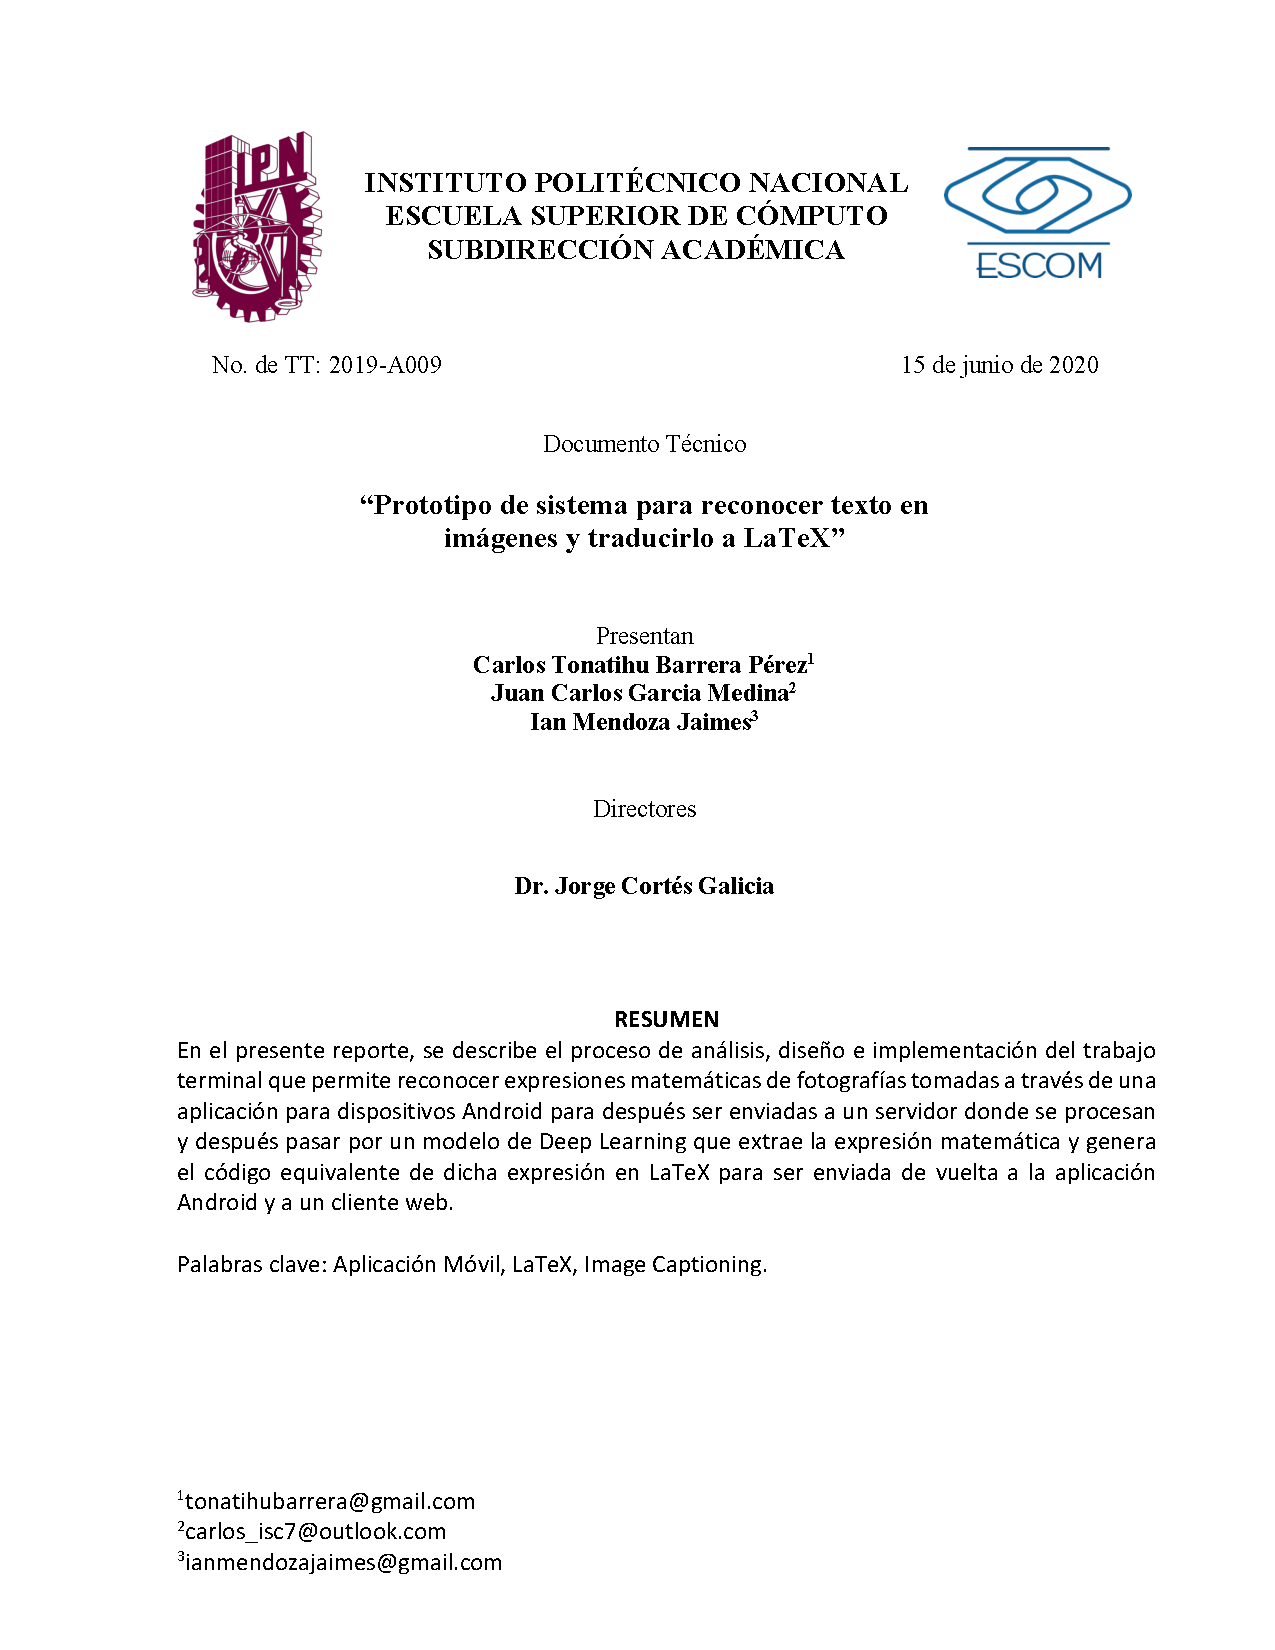
\includegraphics[scale=.85, trim=100 150 100 40]{Disco/HojaPresentacion}
	%left lower right upper
\end{figure}

}
\end{center}
%\vspace{2.5cm}

	
                   % Usada como hoja de presentación
 %
\begin{comment}
\begin{dedication}
A la Facultad de Ingeniería y a la  Universidad, por la formación que me han dado.\\
Es gracias a ustedes que es posible el presente trabajo.\\
En verdad, gracias.\\
Yo.
\end{dedication}
\end{comment}

\begin{alwayssingle}
	{
		\pagestyle{empty}
		%\begin{center}
		%\vspace{1.5cm}
		\begin{figure}[H]
			\centering
			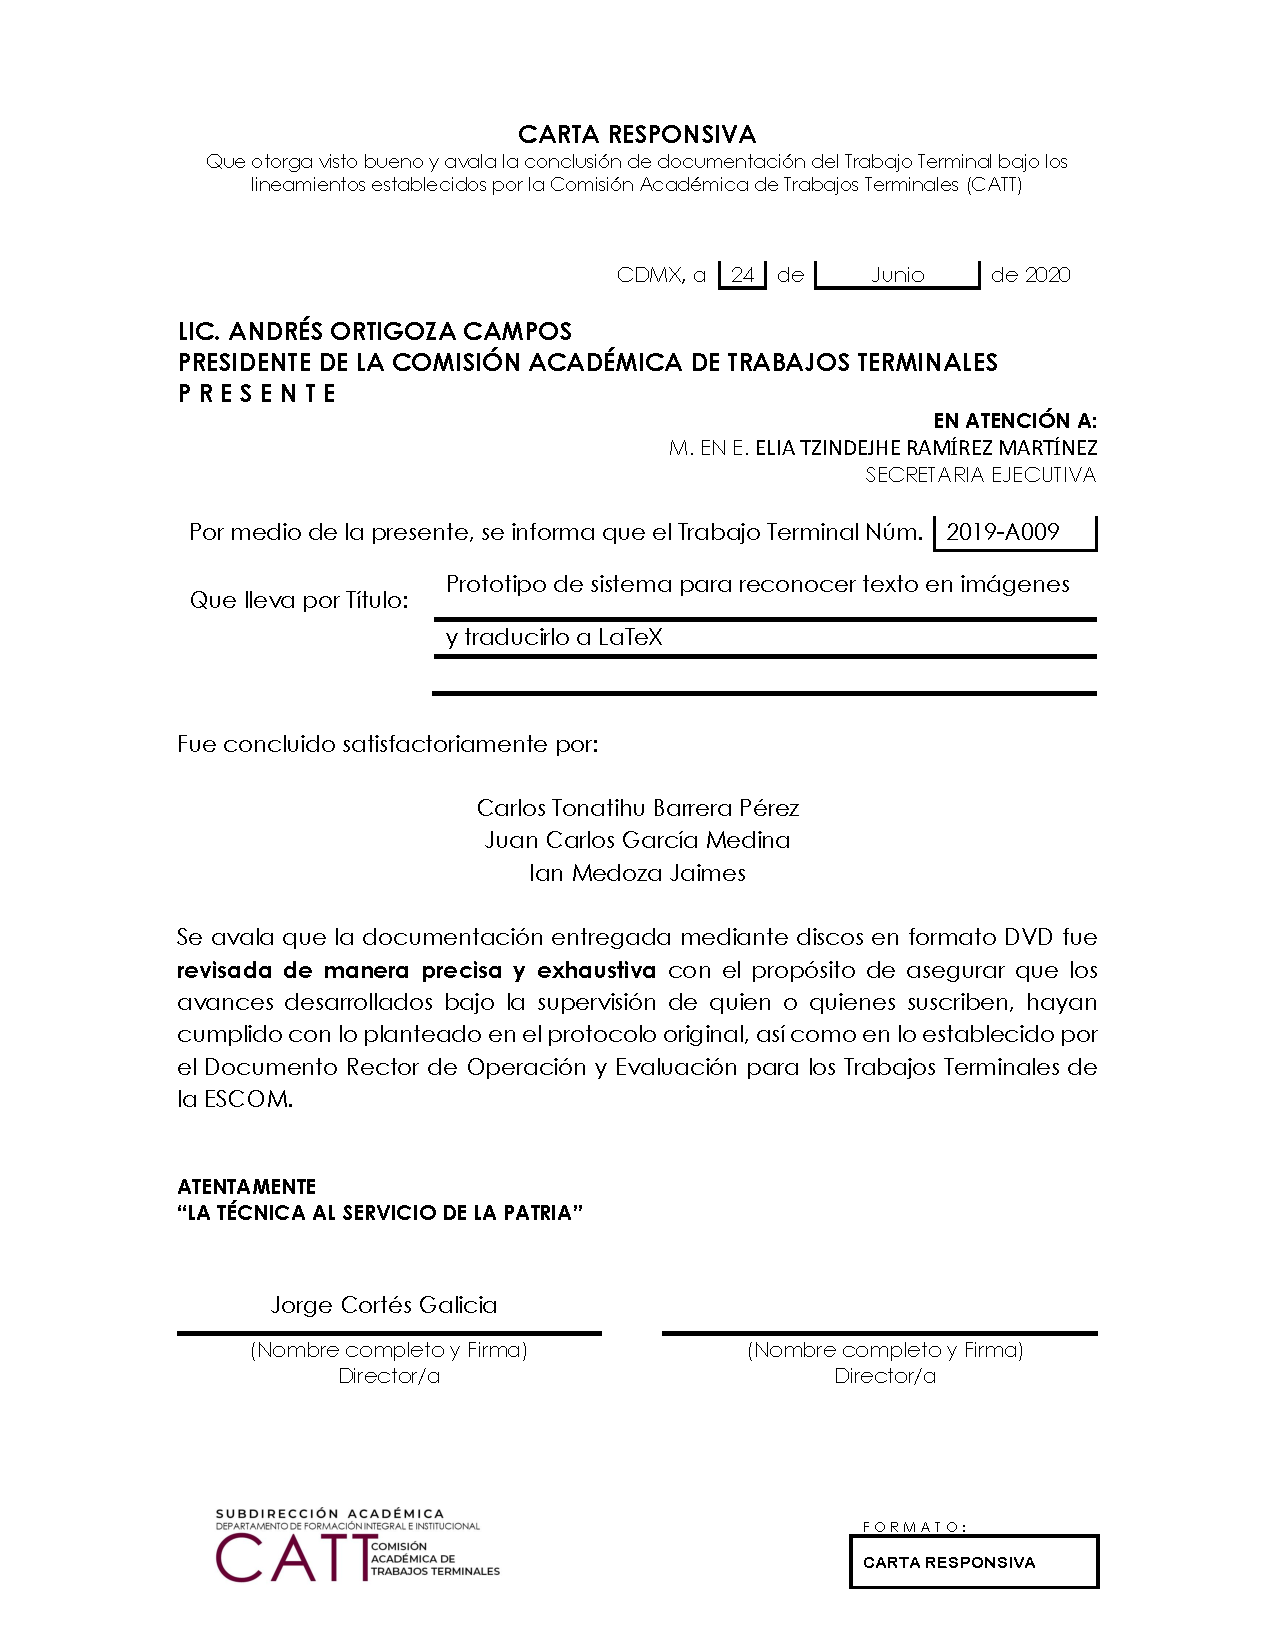
\includegraphics[trim=100 150 100 0, scale=.75]{Disco/carta_responsiva.pdf}
			%left lower right upper
		\end{figure}
		%\end{center}
		%\vspace{0.5cm}
	}
	
\end{alwayssingle}       % Usada como carta responsiva
 %% ******************************* Thesis Declaration ********************************

\begin{comment}
\begin{declaration}

Por la presente declaro que, salvo cuando se haga referencia específica al trabajo de otras personas, el contenido de esta tesis es original y no se ha presentado total o parcialmente para su consideración para cualquier otro título o grado en esta o cualquier otra Universidad. Esta tesis es resultado de mi propio trabajo y no incluye nada que sea el resultado de algún trabajo realizado en colaboración, salvo que se indique específicamente en el texto. 

\end{declaration}
\end{comment}

\begin{alwayssingle}
	\pagestyle{empty}
	\begin{center}
		\vspace*{1.5cm}
		\begin{figure}[H]
			\centering
			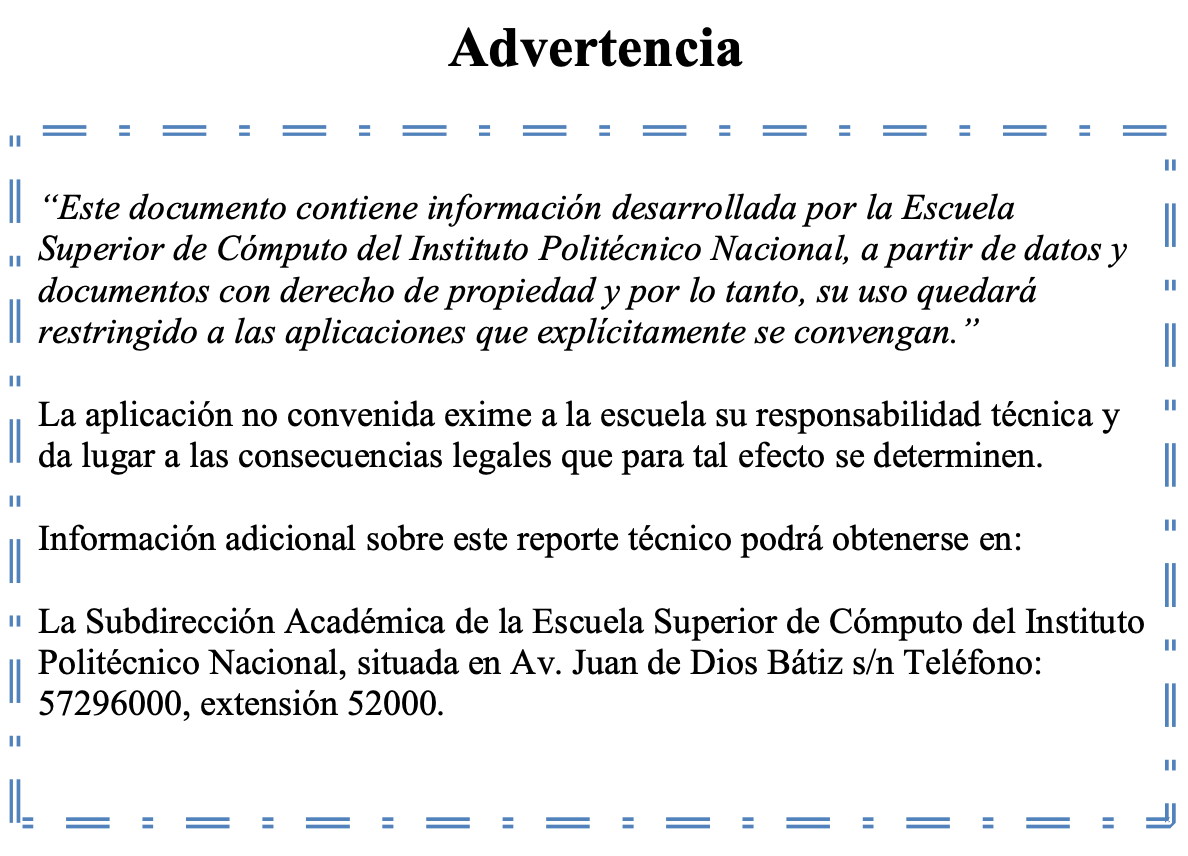
\includegraphics[width=\textwidth]{Disco/advertencia}
		\end{figure}
	\end{center}
	%\vspace{0.5cm}
\end{alwayssingle}
           % Advertencia
 %%\chapter*{}
%\pagenumbering{Roman}

\begin{comment}
\begin{acknowledgements}

También quisiera reconocer a ... por ...CONACYT,  PAPIIT / etc.
\end{acknowledgements}
\end{comment}

\begin{alwayssingle}
	{
		\pagestyle{empty}
		%\begin{center}
		\vspace{1.5cm}
		{\chapter*{Agradecimientos}
			\noindent 
			\textit{``A mis padres Lorena y Miguel, quienes siempre me han brindado su amor y apoyo incondional y a quienes debo enteramente la persona que soy.''} \\
			\\
			\textit{``A mi hermana Natzue, por estar siempre presente acompañandome a lo largo de todo este camino.''}
			\begin{flushright}
				Ian Mendoza Jaimes
			\end{flushright}
			\noindent 
			\textit{``A mis padres, con quienes estaré eternamente agradecido por haberme apoyado incondicionalmente en todo momento durante mi carrera profesional'' }\\
			\\
			\textit{ ``A todos los profesores que me formaron y al Instituto Politécnico Nacional por brindarme la educación que hoy me define como profesionista''.}
			\begin{flushright}
				Juan Carlos Garcia Medina
			\end{flushright}
			\noindent 
			\textit{``Dedicatoria 3''}
			\begin{flushright}
				Persona 3
			\end{flushright}
			
		}
		%\end{center}
		%\vspace{0.5cm}
	}
	
\end{alwayssingle}



   % Los agradecimientos

%%%%%%%%%%%%%%%%%%%%%%%%%%%%%%%%%%%%%%%%%%%%%%%%%%%%%
%                   ÍNDICES                         %
%%%%%%%%%%%%%%%%%%%%%%%%%%%%%%%%%%%%%%%%%%%%%%%%%%%%%
%Esta sección genera el índice
\setcounter{secnumdepth}{3} % organisational level that receives a numbers
\setcounter{tocdepth}{3}    % print table of contents for level 3
\tableofcontents            % Genera el índice 
%: ----------------------- list of figures/tables ------------------------
\listoffigures              % Genera el ínidce de figuras, comentar línea si no se usa
\listoftables               % Genera índice de tablas, comentar línea si no se usa

%%%%%%%%%%%%%%%%%%%%%%%%%%%%%%%%%%%%%%%%%%%%%%%%%%%%%
%                   CONTENIDO                       %
%%%%%%%%%%%%%%%%%%%%%%%%%%%%%%%%%%%%%%%%%%%%%%%%%%%%%
% the main text starts here with the introduction, 1st chapter,...
\mainmatter
\def\baselinestretch{1.5}                   % Interlineado de 1.5
\chapter{Introducción}
% Esta sección es en su mayoría lo que ya esta en el protocolo
% por lo que si se van a hacer correcciones en el protocolo hay mantener esta sección y el protocolo con la información más reciente.
% Las secciones que en teoria aparecen aqui son:
% \begin{itemize}
%     \item Resumen
%     \item Palabras clave
%     \item Antecedentes
%     \item Justificación
%     \item Planteamiento del problema
%     \item Objetivos
%     \item Estado del arte
%     \item Descripción del documento
% \end{itemize}

%{palabras clave, planteamiento del problema[incluye: antecedentes, justificación], objetivos, estado del arte, propuesta}

%\begin{itemize}
%    \item Palabras Clave
%    \item Planteamiento del problema
%    \item Objetivos
%    \item Estado del arte
%    \item Descripción del documento
%\end{itemize}


LaTeX es un sistema de tipografía de alta calidad que incluye características útiles para el diseño de documentos técnicos y científicos. Este software, es de facto un estándar para la comunicación y la publicación de artículos científicos. %\cite{Agregar Citas}.
\bigskip

A pesar de lo práctico que puede ser LaTeX, si el documento contiene muchas expresiones matemáticas, puede resultar tedioso para el usuario escribir dichas expresiones. Por lo que este Trabajo Terminal tiene como finalidad brindar una herramienta que permita amenizar la interacción de nuevos usuarios al escribir expresiones matemáticas en LaTeX mediante el uso de una aplicación móvil y una aplicación web, esta última capaz de reconocer expresiones matemáticas en imágenes que pueden ser tomadas desde el mismo \texttt{smartphone}.
\bigskip

 %siento que faltan
\newpage
\section{Planteamiento del problema}
En la actualidad no existe un sistema que permita reconocer expresiones matemáticas tomando como entrada una fotografía para su posterior traducción a LaTeX, si bien en los últimos años la investigación ha permitido que haya avances en cuanto al reconocimiento y traducción de expresiones matemáticas, al tener un enfoque de investigación se quedan como modelos fuera de lo práctico y los pocos existentes como se muestra en el estado del arte \ref{tab:state_of_art} trabajan con entradas ideales como son expresiones escritas desde dispositivos tales como tabletas digitalizadoras o plumas electrónicas sin considerar entradas como pueden ser fotografías tomadas por un smartphone en las que la resolución varía de dispositivo a dispositivo eliminando un tamaño fijo de la entrada y otros elementos como el ruido que puede incorporarse al momento de la toma de la fotografía que afectan el reconocimiento de las expresiones matemáticas. Además, no cuentan con un control sobre dichas traducciones que se realizan o sobre los usuarios.
\\\\

%\textbf{JUSTIFICACIÓN}

El enfoque del presente trabajo terminal consiste en desarrollar un sistema conformado por una aplicación tanto móvil como web que en conjunto permitan tomar fotografías y extraer las expresiones matemáticas para su posterior traducción incluyendo la capacidad de gestionar las traducciones incluyendo la clasificación de las mismas mediante usuarios y proyectos asociados a dichas traducciones.
\\\\%\bigskip

Con el desarrollo de este prototipo de sistema se debe tener en cuenta que específicamente se ataca el problema de expresiones matemáticas (que a diferencia del reconocimiento de texto plano el cual es un problema que se considera resuelto por los buenos resultados que se han obtenido) este sigue siendo un problema abierto debido a su naturaleza jerárquica y bidimensional y que en la actualidad las soluciones existentes no brindan buenos resultados aún \cite{chino}, por lo que mejorar los resultados del estado del arte no es el objetivo de este trabajo.
%\\\\%\bigskip
%El tiempo estimado de desarrollo del Trabajo Terminal es de diez meses, empezando en el mes de agosto 2019 y concluyendo en el mes de mayo del 2020 


\newpage

\section{Estado del arte}

%ESTADO DEL ARTE
Algunos sistemas similares que se han desarrollado son:
\begin{itemize}
	\item Mathphix \cite{mathphix}%
	\item MyScript Nebo \cite{nebo}%[Cita].
	\item SESHAT \cite{AlvaroPR16}%[4].
	\item IDEAL Math Writer \cite{idmath} %[5].
\end{itemize}
Los cuales se describen en la tabla \ref{tab:state_of_art}: \\\\
\begin{longtabu} to 1\textwidth { | X[m,c] | X[m,c] | X[m,c] | }
	\hline
	\textbf{SOFTWARE} & \textbf{CARACTERISTICAS} & \textbf{PRECIO EN EL MERCADO} \\
	\hline
	Mathpix  & Es una aplicación de escritorio en la que puedes usar un comando para tomar una captura de pantalla y convertir el texto capturado a LaTeX. También cuenta con un API de pago  & Este producto cuenta con diferentes planes de pago según su uso o el tiempo que decidas pagarlo. Tiene distinto trato para empresas. Un ejemplo de suscripción mensual es \$99 dólares el mes.  \\
	\hline
	MyScript Nebo  & Es una aplicación Android que transforma el texto escrito en el dispositivo en texto digital. Incluye soporte para ecuaciones. Es necesario el uso de una pluma digital.& \$189.00 en Google Play Store  \\
	\hline
	Mathpix  & Es una aplicación de escritorio en la que puedes usar un comando para tomar una captura de pantalla y convertir el texto capturado a LaTeX. También cuenta con un API de pago  & Este producto cuenta con diferentes planes de pago según su uso o el tiempo que decidas pagarlo. Tiene distinto trato para empresas. Un ejemplo de suscripción mensual es \$99 dólares el mes.  \\
	\hline
	SESHAT  & Es un proyecto de doctorado de la Universidad Politécnica de Valencia open source. Convierte el texto de imágenes en texto digital y en formato LaTeX. Soporta ecuaciones. Necesita ser instalado mediante terminal en Linux. & No es una aplicación comercial  \\
	\hline
	\caption{Resumen de productos similares}
	\label{tab:state_of_art}
\end{longtabu}


\section{Objetivos}
\subsection{Objetivo general}
Desarrollar un sistema que reconozca un conjunto delimitado de tipos de expresiones matemáticas en una imagen dada y las traduzca a un formato que un compilador de LaTeX pueda procesar, el conjunto de entrenamiento se encuentra delimitado en el capítulo de análisis.
\subsection{Objetivos específicos}
\begin{enumerate}
	\item Desarrollar una aplicación móvil que permita tomar fotografías y que pueda conectarse a una aplicación web para su posterior procesamiento.
	\item Desarrollar un módulo de análisis de imágenes para el reconocimiento de las expresiones matemáticas.
	\item Desarrollar un módulo de traducción a LaTeX.
	\item Desarrollar la interfaz que conecte el módulo de análisis de imágenes alojado en el servidor con la aplicación móvil y web.
\end{enumerate}


\section{Resultados esperados}
Podemos separar el sistema en dos bloques principales, el primero el lado del cliente el cual se compondrá de la aplicación móvil y de la interfaz web con las cuales el usuario podrá interactuar. Por otro lado, se tiene la parte del servidor web que se conectará con la aplicación móvil, en el servidor se encontrará la parte de análisis de imágenes junto con el módulo de traducción. Finalmente se tiene el módulo de gestión de usuarios. Esto se puede apreciar en la Figura \ref{fig:arquitecturaInicial}.%ref %%AYUDA, NO ESTA REFERENCIANDO

El sistema se compone de cinco módulos:
\begin{enumerate}
    \item Módulo de análisis de imágenes. Este módulo se encargará de procesar las imágenes e identificar un conjunto delimitado de tipos de expresiones matemáticas.
    \item Módulo de traducción. Este módulo tomará como entrada lo obtenido en la etapa de análisis de imágenes y regresará el respectivo código de LaTeX que represente las expresiones matemáticas reconocidas.
    
    \item Módulo de gestión de usuarios. En este módulo se hará la gestión de la información de los usuarios de la aplicación, lo que implica tener un control de su información y de los archivos que generen al usar el sistema. Esta gestión de usuarios estará presente tanto en la aplicación móvil como en el servidor web.

    \item Aplicación móvil. Este módulo consiste en el desarrollo de la aplicación móvil que el usuario final llevará en su Smartphone y con la cual podrá tomar fotos que cumplan ciertos requisitos para así obtener el código en LaTeX a través de la comunicación con la aplicación web.

    \item Servidor web. El servidor web hará uso de los módulos de análisis de imágenes, de traducción y de gestión de usuarios por lo que deberá de mantener una comunicación entre ellos y la aplicación móvil, así como con la base de datos. Además, es el punto que permite visualizar el resultado final de todo el procesamiento de imágenes a través de una interfaz web.
\end{enumerate}
Los productos esperados del Trabajo Terminal son:
\begin{enumerate}
    \setcounter{enumi}{5}
    \item Código fuente del trabajo desarrollado (todos los módulos).
    \item Documentación técnica del sistema.
\end{enumerate}

\begin{figure}[h]
\centering
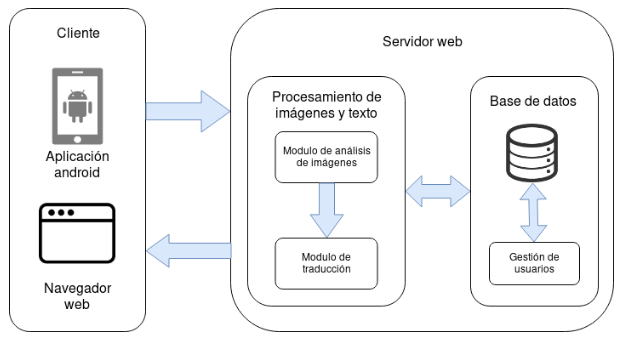
\includegraphics[width=1.0\textwidth]{capitulo1/images/arquitectura.png}
\caption{Arquitectura del sistema.}
\label{fig:arquitecturaInicial}
\end{figure}
\newpage

\section{Metodología} Para el desarrollo del proyecto se eligió la metodología incremental debido a que permite dividir el proyecto en pequeños incrementos \cite{iterativeDevelopment}. Este modelo nos permite flexibilidad a la hora de decidir que requerimientos funcionales se trabajaran primero, es decir, primero se trabajan aquellos con mayor prioridad en los primeros incrementos del sistema para después trabajar el resto o realizar un análisis más profundo a dichos requerimientos de incrementos futuros \cite{sommerville}. De esta forma, se plantean los siguientes incrementos con el objetivo de que al final de cada uno de estos se obtenga la funcionalidad requerida y validar que lo que se trabajo sea correcto para que al final de todos los incrementos se tenga el sistema completo.
\begin{itemize}
	\item Se desarrollará la aplicación móvil la cual su principal funcionalidad es la obtención de las imágenes y su comunicación con el servidor web.
	\item Se desarrollará la aplicación web ya que es lo que nos servirá para conectar con la aplicación móvil con el resto de los módulos que se desarrollaran en un futuro.
	\item Se hará la integración entre la aplicación móvil y la aplicación web.
    \item Se detallaran a fondo requerimientos si es necesario, se realizara el análisis y diseño del módulo de análisis de imágenes, construcción del módulo y finalmente se harán pruebas sobre este.
    \item El módulo de traducción va de la mano con el módulo anterior, al tener esto listo y con sus respectivas validaciones aprobadas se realizará el desarrollo y con ello realizar pruebas sobre todos los componentes que se tengan hasta este punto.
    \item Este incremento final tendrá como objetivo el integrar todo lo desarrollado hasta este punto.
\end{itemize}




%----------------------------OBJETIVOS

\newpage


% Ya hay muchos trabajando en este tema utilizando redes neuronales, lo interesante del nuestro es ponerlo en una aplicación web/android 

% En el entrenamiento se pueden probar varias funciones de cada capa de la arquitectura. 

% Wandb logro un resultado mejor que el del estado del arte, es decir, mejor que el articulo de harvard 

% Los resultados son buenos con imagenes preprocesadas del conjunto de entrenamiento, en imagenes que se esperan de usuarios no es tan bueno el resultado. 

% ¿El estado del arte ataca ecuaciones a mano o solo screenshots? Esto es importante a considerar si nos basamos en estos trabajos para el nuestro. 

% El preprocesamiento de la imagen se puede atacar con dos posibles formas, esto puede ser la parte de nuestro TT que sea la innovadora 

% El preprocesamiento de la imagen nos va a matar con Benoso. 

% Una amenaza es wandb entre otros investigadores igual es importante tomarlo en cuenta para la factibilidad ya que en cualquier momento pueden surgir nuevos avances y dejarnos obsoletos 

% Quiubole con que si utilizan un latex parser para la normalizacion 

% No manches hay muchos trabajos al respecto de gente pro =( 

% Hay un chingo de terminos que no entiendo 

% Todo lo hacen con un conjunto de entrenamiento ya preprocesado nada de input de usuario 

\chapter{Marco teórico}
Con el desarrollo del sistema producto del presente trabajo terminal se involucran ciertos conceptos provenientes en su mayoría de ramas de ciencias de la computación y en general en alusión a la Inteligencia Artificial, por lo que es conveniente dar contexto sobre los elementos necesarios para el desarrollo del trabajo terminal.
\section{Análisis de Imágenes}
        El análisis de imágenes comprende un conjunto de operaciones sobre una o varias imágenes con el propósito de obtener una imagen con mayor realce o para extraer características útiles, es un tipo de dispensación de señales en el que la entrada es una imagen y la salida puede ser otra imagen o características asociadas a la imagen, algunos de los pasos generales se describen a continuación:
        
        \subsection{Preprocesamiento}
            Preprocesamiento es un nombre común para operaciones con imágenes al más bajo nivel de abstracción. Tanto entrada como salida son imágenes de intensidad. Estas imágenes tienen el mismo tipo de datos que la original, con una imagen de intensidad usualmente representada por una matriz de valores de función de imagen (Brillo) El objetivo de preprocesar es la mejora de los datos de la imagen que borre distorciones o realce características importantes para procesamiento posterior, incluso las transformaciones geométricas de las imagenes e.g (rotación, escalamiento y traslación) son también clasificadas como métodos de preprocesamiento, ya que técnicas similares son utilizadas \cite{imgAnalySeg}.
               
                
        \subsection{Realce de la imagen}
            El objetivo principal de realce de imagen es también procesar una imagen dada tal que el resultado sea mas ajustable que la imagen original para aplicaciones específicas. Por ejemplo para la remoción de ruido.
            \\\\%\bigskip
            Acentúa o afina características de la imagen como ejes, límites o contraste para hacer un despliegue gráfico mas útil para el análisis.
            \\\\%%\bigskip
            El realce no incrementa o decrementa el contenido de la información inherente de los datos pero sí incrementa el rango dinámico de las características elegidas de tal modo que puedan ser detectadas fácilmente.
            \\\\%\bigskip
            Proveé \'mejor\' entrada para otras técnicas avanzadas de procesamiento automatizadas de imágenes.
                        
        \subsection{Segmentación de la imagen}
            El término segmentación utilizada en el contexto de análisis de imágenes se refiere a la partición de una imagen en un conjunto de regiones que la cubren. El objetivo en muchas de las tareas es que para las regiones se representen áreas significativas de la imagen, como áreas urbanas, fronteras o bosques de una imagen satelital. En otras tareas de análisis, las regiones pueden ser conjuntos de bordes de pixeles agrupados en estructuras como segmentos de líneas y segmentos de arcos circulares en imágenes de objetos industriales en 3D. Las regiones pueden también estar definidas como grupos de pixeles teniendo ambos un borde y una forma particular como un circulo o una elipse or polígono. Cuando las regiones de interés no cubren la imagen completa, aún se requiere el proceso de segmentación en regiones de y de fondo para ignorarse. 
            \cite{imgAnalySeg}
            %REF courses.cs.washington.edu/courses/cse576/book/ch10.pdf
            \begin{figure}[H]
                \centering
                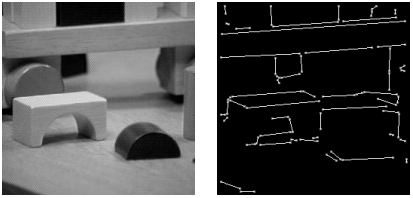
\includegraphics[width=0.7\textwidth]{capitulo2/images/segmentation.PNG}
                \caption{Imagen con bloques (Izquierda) y conjunto de segmentos de linea extraídos (Derecha).}
                \label{fig:segmentacion}
            \end{figure}
        \subsection{Extracción de características}
            
            %http://citeseerx.ist.psu.edu/viewdoc/download?doi=10.1.1.375.6848&rep=rep1&type=pdf
        \subsection{Clasificación e interpretación}
            %http://citeseerx.ist.psu.edu/viewdoc/download?doi=10.1.1.375.6848&rep=rep1&type=pdf


\section{Métodos de reconocimiento de expresiones matemáticas}
\subsection{Análisis sintáctico dirigido}
Los lenguajes libres de contexto, son aquellos que tienen una notación recursiva natural llamada \textit{gramática libre de contexto}. Por ende, un lenguaje libre de contexto es todo aquel que puede ser representado por una gramática libre de contexto.

Una gramática libre de contexto G, queda definida de la siguiente manera:

\begin{equation}
    G = (V, T, P, S)
\end{equation}

de donde, V es el conjunto de variables, T el conjunto de símbolos terminales, P el conjunto de producciones y S el punto de inicio \cite{automata}.

El lenguaje matemático, es decir, las expresiones matemáticas son un lenguaje libre de contexto. Esto quiere decir que es posible definir una gramática libre de contexto para definir a las expresiones matemáticas. Esta es una práctica muy común en la teoría de compiladores.

Sabiendo esto, una aproximación a la resolución del problema de reconocer expresiones matemáticas en imágenes es la que describe \cite{gramaticasAnderson}. El método consiste en dos etapas:

\begin{itemize}
    \item Reconocimiento de caracteres: Utilizar algún método de reconocimiento de patrones para localizar los caracteres y anotar sus coordenadas. 
    \item Análisis sintáctico dirigido: Utilizar la etapa previa para determinar la jerarquía, basándose en un conjunto de reglas definidas (las gramáticas libres de contexto).
\end{itemize}

En la Figura \ref{fig:gramaticas}, se puede ver un ejemplo del proceso de reconocimiento propuesto por este método.

\begin{figure}[h]
    \centering
    \subfigure[]{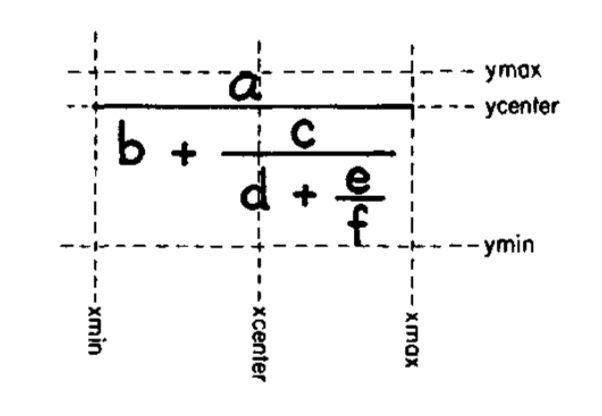
\includegraphics[width=6cm]{capitulo2/images/gramaticas1}}
    \subfigure[]{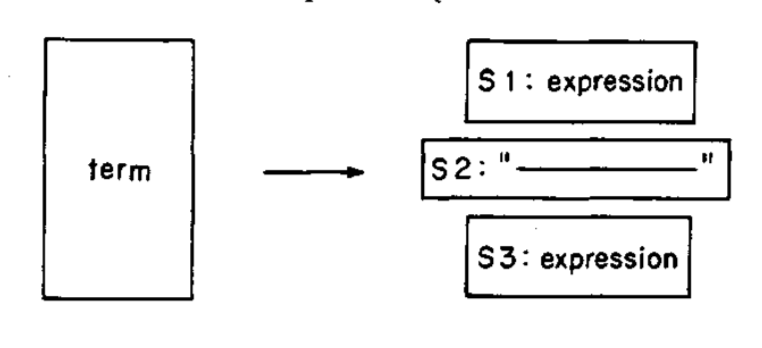
\includegraphics[width=6cm]{capitulo2/images/gramaticas2}}
    \caption{\textbf{a)} La primera etapa del método de reconocimiento, se anotan las coordenadas de de cada caracter. \textbf{b)} Se realiza un análisis sintáctico con las gramáticas libres de contexto definidas.}
    \label{fig:gramaticas}
\end{figure}

\newpage
\subsection{Redes Neuronales}
    Existe un tipo de neurona artificial llamada perceptrón desarrolladas entre 1950 y 1960 por el científico Frank Rosenblatt, sin embargo este modelo ha ido evolucionando y hoy en día se utilizan otros modelos de neurona como el llamado sigmoid neuron, que para entender, primero se debe definir al perceptrón como modelo.
    Un perceptrón toma varias entradas binarias $x_{1},x_{2},x_{3},...,x_{n}$ y produce una sola salida binaria:
     \begin{figure}[H]
        \centering
        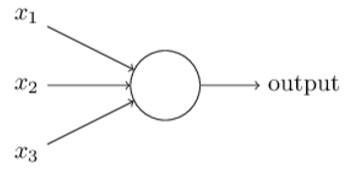
\includegraphics[width=0.5\textwidth]{capitulo2/images/perceptron.PNG}
        \caption{Representación de un percetrón con entradas $x_{1}$, $x_{2}$ y $x_{3}$}
        \label{fig:perceptron}
    \end{figure}
    La regla que Rosenblatt introdujo para calcular la salida involucra valores llamados pesos $w_{1},w_{2},w_{3},...$ que pueden tomar valores reales expresando la importancia de las respectivas entradas a la salida, la salida de la neurona (0 o 1) es determinado por la suma ponderada $\sum_{j} w_{j} x_{j}$ es menor o igual a un valor de umbral. Así como los pesos, el valor de umbral es un número real el cuál es un parámetro de la neurona:
     \begin{equation}
        output = \left\{ \begin{array}{lcc}
             0 &   si  & \sum_{j} w_{j} x_{j} \leq threshold \\
             \\ 1 &  si & \sum_{j} w_{j} x_{j} \ge threshold\\
             \end{array}
        \right.
    \end{equation}
    \newpage
    Una red neuronal es una red de perceptrones que agrega complejidad a las decisiones.
    \begin{figure}[H]
        \centering
        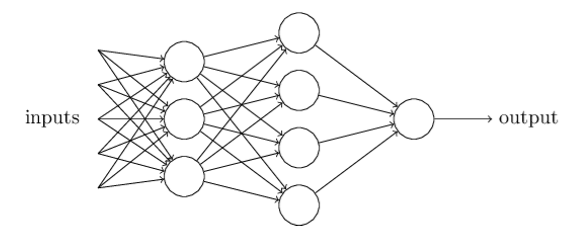
\includegraphics[width=1\textwidth]{capitulo2/images/NNmodel.PNG}
        \caption{Red neuronal de 3 capas}
        \label{fig:NNmodel}
    \end{figure}
    \subsubsection{Conjunto de entrenamiento}
    El conjunto de entrenamiento es un conjunto de datos que se utiliza a modo de ejemplo para que un modelo pueda aprender. En el aprendizaje supervisado el conjunto de entrenamiento se compone de muchas tuplas (X,Y) siendo X un vector de características del problema y Y un vector del resultado al que queremos llegar \cite{deeplearningbook}.
    
    
    \subsubsection{Aprendizaje Profundo}
        El aprendizaje profundo de forma clásica se refiere al tratamiento de redes neuronales con mas de dos capas, sin embargo, debido al cambio que esta sub-area ha sufrido, se debe definir como el tratamiento de redes neuronales con un largo número de parámetros y capas en una de las cuatro arquitecturas de redes fundamentales:
        \begin{itemize}
            \item Redes pre-entrenadas no supervisadas
            \item Redes Neuronales Convolucionales
            \item Redes neuronales recurrentes
            \item Redes neuronales recursivas.
        \end{itemize}
    
    Siendo las Redes Neuronales Convolucionales de las que se expondrá a detalle en  \\%siguiente subseccion.
    \\Una de las propiedades mas importantes que permite el Aprendizaje Profundo es la extracción automática de características que puede ser clave en dicho paso del análisis de imágenes.
    
    \subsubsection{Redes Neuronales Convolucionales}
    Las redes neuronales convolucionales han ganado popularidad en los últimos años debido a su efectividad prometedora en el aprendizaje profundo. Partiendo por el procesamiento de imágenes, las capas convolucionales han encontrado su camino en otros subcampos del aprendizaje profundo y muestran éxito en la mayor parte de dichos campos.\\\\ 
    La diferencia fundamental entre \textit{fully connected} (completamente conectadas) y \textit{convolutional neural networks}(redes neuronales convolucionales) es el patrón de conexión entre las capas consecutivas. En el caso de las completamente conectadas como el nombre lo sugiere, cada unidad es conectada a todas las unidades de la previa capa. \\\\
    En una capa convolucional de una red neuronal, por otra parte, cada unidad está conectada a (típicamente pequeña) un número de unidades cercanas en la capa previa. Más aún, todas las unidades están conectadas a la capa previa de la misma forma con los pesos exactamente iguales y estructura. Esto lleva a una operación conocida como convolución, dando a la arquitectura este nombre, a grandes rasgos esto significa aplicar una pequeña "ventana" de pesos (conocida como filtro) sobre una imágen como se muestra en la figura \ref{fig:CNNFilter}.
    
    
     \begin{figure}[H]
        \centering
        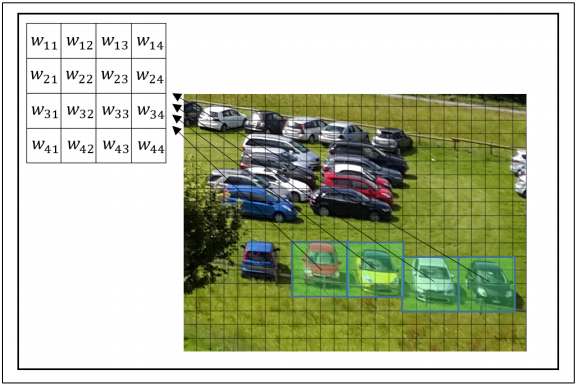
\includegraphics[width=0.7\textwidth]{capitulo2/images/CNN_window.png}
        \caption{Matriz de pesos conocida como ventana aplicada a una imagen.}
        \label{fig:CNNFilter}
    \end{figure}
    \newpage
    
   
  
    \subsubsection{Arquitectura Encoder-Decoder}
    
    En particular se discutirá la arquitectura de Long Short-Term Memory (LSTM). LSTM es una arquitectura de una red neuronal recurrente diseñada para resolver problemas secuenciales, normalmente conocidos como sequence-to-sequence. Los problemas secuenciales, tienen usualmente como reto, predecir el siguiente resultado encontrado. Un reto que surge naturalmente de estos problemas, es la longitud variable de las entradas.
    
    Una aproximación para resolver los problemas secuenciales es el Encoder-Decoder LSTM él cual ha probado ser efectivo en muchos casos. Esta arquitectura se compone de dos modelos \cite{encoderDecoder}:
    
    \begin{itemize}
    	\item Encoder: Es una red neuronal encargada de leer la entrada de longitud variable y convertirla en un vector de longitud fija.
    	\item Decoder: Es una red neuronal encargada de tomar la salida del Encoder y como salida obtiene un valor predecido.
    \end{itemize} 


	\subsubsection{Image Captioning}
    
    Es una rama emergente del \textit{deep learning} que ha ido ganando atención en los últimos años. Este campo es un punto intermedio entre la vision por computadora y el procesamiento del lenguaje natural. El actual estado del arte en image captioning tiene una aproximación similar a los modelos sequence-to-sequence, los cuales utilizan una arquitecura Encoder-Decoder \cite{imagetolatex}.
    
    Si se trata al problema de reconocer expresiones matemáticas en imagenes como un problema sequence-to-sequence de image captioning, se puede emplear una arquitectura de Encoding-Decoding para hacer la conversión de la imagen a LaTeX de manera directa. Esto permite a la red manejar imagenes de longitud variable y reconocer los símbolos a la vez que va reconociendo las expresiones.
    
    La arquitectura que se esta utilizando actualmente para solucionar este problema se muestra en la Figura \ref{imgcaptioning} \cite{imagetolatex}\cite{imagemarkup}\cite{chino}.
    
    \begin{figure}
		\centering
		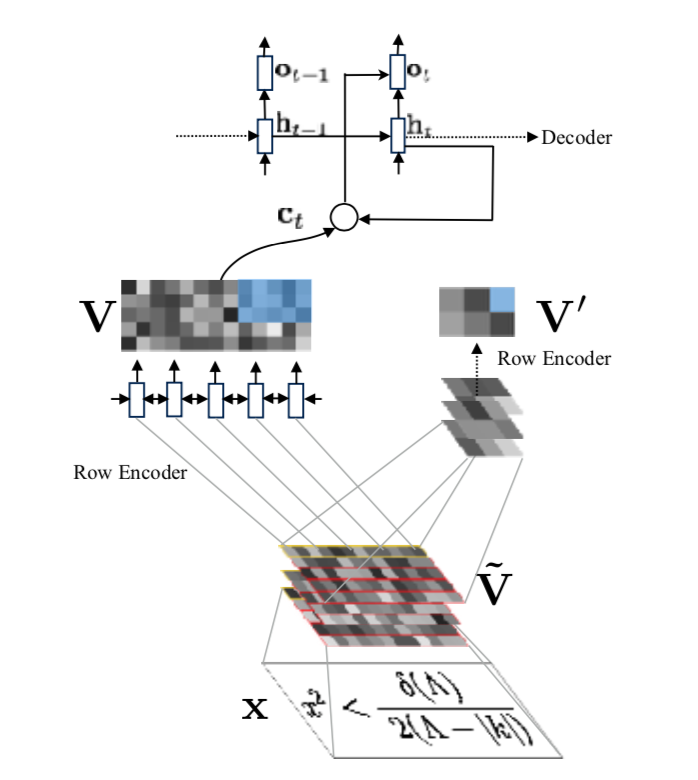
\includegraphics[width=8cm]{capitulo2/images/imgcaptioning}
		\caption{Arquitectura de image captioning para reconocer expresiones matemáticas en imagenes.}
		\label{fig:imgcaptioning}
    \end{figure}

\subsection{Análisis estructural}

Este método coincide con el primero en que debe de utilizar una técnica de reconocimiento de patrones para etiquetar primero los símbolos. Las etiquetas que utiliza tienen que ver son su posición en la imagen, así como su tamaño. 

La diferencia en este método, radica en su segunda etapa. No se realizará un análisis con gramáticas, en su lugar se intentara deducir la estructura jerárquica con algún otro método. El artículo \cite{spanningtree} propone utilizar el algoritmo de Kruskal para obtener un árbol de recubrimiento mínimo por niveles, de este modo se puede saber la estructura de la expresión matemática recorriendo el gráfo resultante.La Figura \ref{fig:spanningtree} muestra un ejemplo de como funciona este método.

\begin{figure}[h]
	\centering
	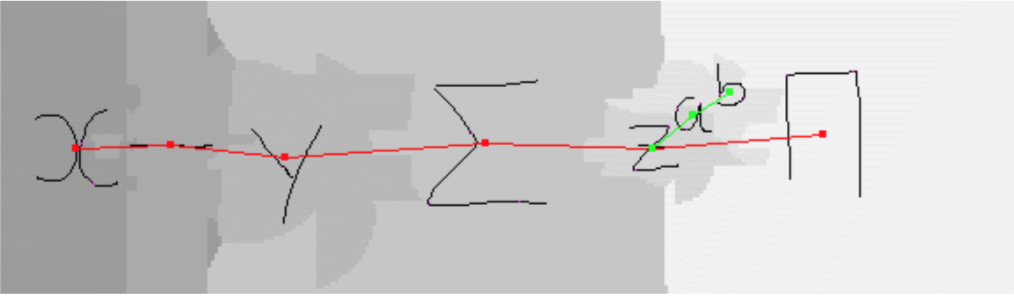
\includegraphics[width=8cm]{capitulo2/images/spanningtree}
	\caption{Utilización de un árbol de recubrimiento mínimo para el reconocimiento de expresiones matemáticas.}
	\label{fig:spanningtree}
\end{figure}
\newpage
\subsection{Aprendizaje profundo como servicio}
El entrenamiento de redes neuronales profundas, conocidas como aprendizaje profundo es en la actualidad áltamente complejo computacionalmente. Requiere un sistema con la combinación correcta de software, drivers, memoria, red y recursos de almacenamiento, por factores como estos los proveedores de cloud computing como Amazon Web Services, Microsoft Azure o Google Cloud ofrecen actualmente servicios de Machine Learning proveyendo API's como pueden ser de entrenamiento de modelos o de visualización de datos y generación de estadísticas, permitiendo que desarrolladores y científicos de datos se enfoquen mas en tareas como el entrenamiento de modelos, análisis de datos, etc.
\\\\
Los modelos de aprendizaje profundo requieren de un proceso experimental e iterativo, requiriendo cientos e incluso miles de ejecuciones que requieren de un amplio poder de cómputo para encontrar la combinación correcta de las configuraciones e hiper-parámetros de la red neuronal. Esto puede tomar semanas o incluso meses y este tipo de servicios garantiza una disponibilidad en todo momento y en conjunto permite que un sistema completo esté dividido en módulos consiguiendo que el mantenimiento y detección de fallos sean tareas más sencillas.
\\\\ 
En la figura \ref{fig:DLAAS} se puede observar la arquitectura de un sistema divido en módulos y que hace uso de herramientas de Machine Learning para dar respuesta a otros módulos del sistema.

\begin{figure}[H]
	\centering
	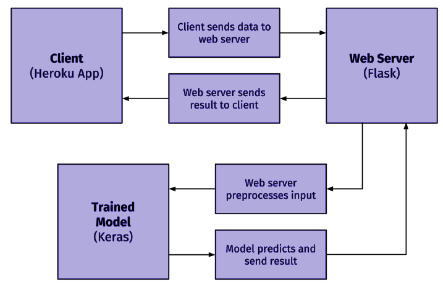
\includegraphics[width=0.7\textwidth]{capitulo2/images/DLAAS.png}
	\caption{Ejemplo de sistema con módulo de Machine Learning}
	\label{fig:DLAAS}
\end{figure}    


\section{Aplicación web}
En la ingeniería de software se denomina aplicación web a aquellas herramientas que los usuarios pueden utilizar accediendo a un servidor web a través de internet o de una intranet mediante un navegador. En otras palabras, es un programa que se codifica en un lenguaje interpretable por los navegadores web en la que se confía la ejecución al navegador \cite{appweb}.

\subsection{Django}
Django es un framework de desarrollo web completamente desarrollado en Python. Permite de una manera rápida poder implementar una aplicación web en el lenguaje Python. Las siguientes, son de las principales características de Django:

\begin{itemize}
    \item \textbf{Rápido}: Tiene como filosofía ayudar a los desarrolladores a crear aplicaciones en el menor tiempo posible.
    \item \textbf{Completo}: Incluye cientos de librerías que permiten ahorrar tiempo y automatizar tareas.
    \item \textbf{Seguro}: Es una de las principales características de Django ya que incluye soluciones a los principales ataques que puede sufrir una aplicación web.
    \item \textbf{Escalable}: Con el patrón de diseño de Django es posible incrementar o decrementar la capacidad de un sitio.
    \item \textbf{Versátil}: Es utilizado por muchas empresas y organizaciones a lo largo del mundo para crear diferentes tipos de proyectos.
\end{itemize}

\subsubsection{Modelo-Vista-Template}
El Modelo-Vista-Template (MTV) es el patrón de diseño que Django implementa. Este patrón es una modificación al conocido Modelo-Vista-Controlador (MVC). La diferencia radica en que Django se encarga de hacer la parte del controlador, por ende el desarrollador solamente tiene que preocuparse por implementar la lógica de negocio y de como mostrará los datos. En la Figura \ref{fig:mtv}, se puede ver una representación del patrón MTV. En el patrón de diseño MTV \cite{mtv}:

\begin{figure}
    \centering
    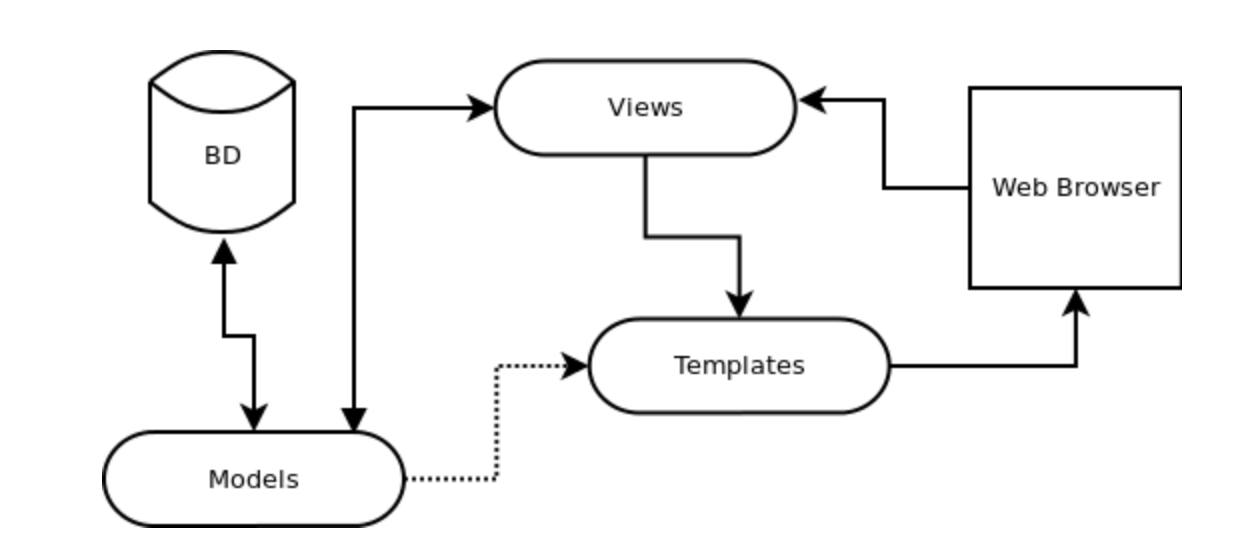
\includegraphics[width=\textwidth]{capitulo2/images/mtv.png}
    \caption{Representación del patrón de diseño Modelo-Vista-Template.}
    \label{fig:mtv}
\end{figure}

\begin{itemize}
    \item \textbf{Modelo}: La capa de acceso a la base de datos. Esta capa contiene toda la información sobre los datos: cómo acceder a estos, cómo validarlos, cuál es el comportamiento que tiene, y las relaciones entre los datos.
    \item \textbf{Template}: La capa de presentación. Esta capa contiene las decisiones relacionadas a la presentación: como algunas cosas son mostradas sobre una página web o otro tipo de documento.
    \item \textbf{Vista}: La capa de la lógica de negocios. Esta capa contiene la lógica que accede al modelo y la delega a la plantilla apropiada: puedes pensar en esto como un puente entre el modelos y las plantillas.
\end{itemize}


\subsection{API REST}
\subsubsection{Application Programming Interface}
Una Interfaz de Programación de Aplicaciones o API es un conjunto de definiciones y protocolos que se utilizan para desarrollar e integrar el software de las aplicaciones.

Las API permiten que sus servicios se comuniquen con otros, sin necesidad de saber como están implementados. Esto simplifica el desarrollo de las aplicaciones y permite ahorrar tiempo y dinero \cite{apiArticle}.
\subsubsection{Represenational State Transfer}

Representational State Transfer (REST) es un estilo de arquitectura basado en un conjunto de principios que describen como recursos interconectados son definidos y direccionados. Estos principios fueron descritos en el año 2000 por Roy Fielding como parte de obtención de su doctorado.
\\
Es importante hacer énfasis en que REST es un \textbf{estilo de software de arquitectura} y no un conjunto de estandares. Como resultado, dichas aplicaciones o arquitecturas son en ocasiones referidas como aplicaciones RESTful o REST-style \cite{restArticle}. 
\\
Una aplicación o arquitectura considerada RESTful o REST-style es caracterizada por:
\begin{itemize}
	\item La funcionalidad y estado son dividiad en recursos distribuidos.
	\item Cada recurso es únicamente direccionable usando un conjunto uniforme y mínimo de comandos (típicamente usando comandos HTTP de GET, POST, PUT o DELETE).
	\item El protocolo es cliente/servidor, stateless, por capas y soporta almacenamiento cache.
\end{itemize} 
 La figura \ref{fig:rest_mess} ilustra el uso de REST para servicios Web.
\begin{figure}[H]
	\centering
	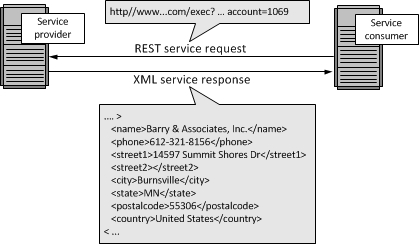
\includegraphics[width=0.5\textwidth]{capitulo2/images/rest_messages.jpg}
	\caption{Consumidor y proveedor de servicios comunicandose mediante solicitudes y respuestas REST.}
	\label{fig:rest_mess}
\end{figure}  
\subsubsection{Autentificación}
Para hablar de autentificación es necesario primero entender la diferencia entre identificación y autentificación, por un lado la identificación es la capacidad de identificar de forma exclusiva a un usuario de un sistema o una aplicación que se está ejecutando, mientras que la autentificación es la capacidad de demostrar que un usuario o una aplicación es quien dicha persona o aplicación asegura ser \cite{authent}.\\\\
Para el caso de una REST API es en muchas ocasiones necesario que se lleve a cabo la autentificación para permitir o denegar el acceso a recursos de un servidor por ejemplo de acuerdo a los permisos concedidos en función de las credenciales de autentificación para así asegurar que los datos sean visibles únicamente a aquellos que proporcionen las credenciales adecuadas y dispongan de los permisos necesarios.


%https://www.ibm.com/support/knowledgecenter/es/SSFKSJ_7.5.0/com.ibm.mq.sec.doc/q009740_.htm
\section{Android}
Esta sección tiene objetivo presentar las principales características en el desarrollo de la aplicación para Android.
\subsection{Arquitectura de la aplicación}
Para el desarrollo de la aplicación se implemento la arquitectura Clean, la cual como ya se ha mencionado antes se ha mencionado se ha vuelto muy popular en el desarrollo de aplicaciones móviles para android debido a que es una solución que produce sistemas que presentan las siguientes características.

\begin{itemize}
    \item Escalables, por lo que se pueden agregar más funcionalidades de forma sencilla.
    \item Presentan modularidad.
    \item Presentan independencia en cuanto a frameworks, interfaz de usuario y bases de datos.
    \item El proyecto es más fácil de mantener por lo que es más sencillo hacer cambios.
\end{itemize}

Al utilizar esta arquitectura el proyecto queda separado en tres capas como se observa en la figura \ref{fig:capas-arquitectura} con lo cual cada una de ellas tiene su propósito definido.

\begin{figure}[h]
    \centering
    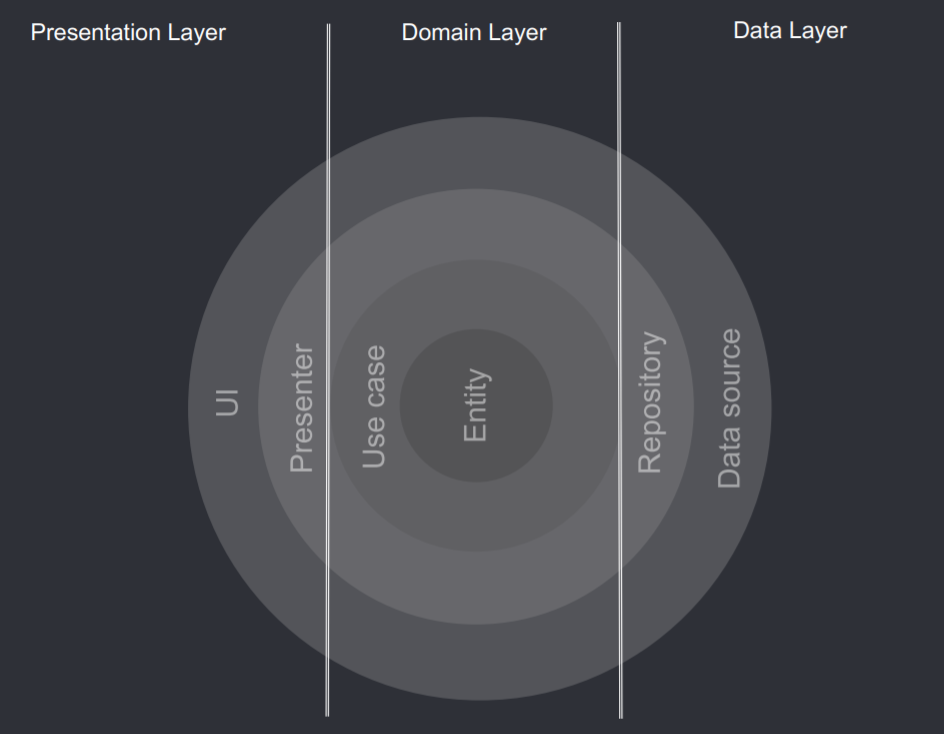
\includegraphics[width=250px]{capitulo5/android/img/capas-clean.png}
    \caption{Tres capas que se tienen al utilizar la arquitectura Clean \cite{cleanGuide}}
    \label{fig:capas-arquitectura}
\end{figure}

\subsubsection{Capa de datos}
La información que se utiliza en el resto de capas proviene de esta capa. Esta capa a su vez se encuentra dividida en la capa de repositorio y en la capa de fuente de datos. 

\paragraph{Capa de repositorio} En esta capa se utiliza el patrón de repositorio como se muestra en la figura \ref{fig:capa-datos}. Gracias a este patrón se puede tener acceso a diferentes fuentes de datos que se encuentran en la capa más baja de nuestra arquitectura, esto nos permite un acceso a los datos de forma transparente para el usuario bajo las condiciones que se presenten.

La forma de utilizar este patrón en la aplicación desarrollado crear una clase en la cual se hace uso de la interfaz que se tiene para el acceso a la fuente de datos. En el siguiente código se puede apreciar el como se crea una instancia de APIService que es nuestra interfaz para fuente de datos.

Después, en nuestro método findAllProyecttosByUser se recupera la información necesaria para mandarla a las capas superiores.

\lstinputlisting[language=Java]{capitulo5/android/src/repositorio.java}

\begin{figure}[h]
    \centering
    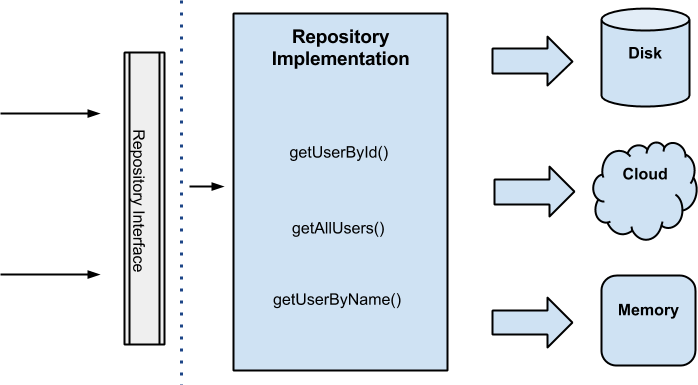
\includegraphics[width=400px]{capitulo5/android/img/capa-datos.png}
    \caption{Capa de datos \cite{cleanWay}}
    \label{fig:capa-datos}
\end{figure}

\paragraph{Capa de fuente de datos} En este trabajo, la fuente de datos que se tiene es un API REST, sin embargo si se requiere acceder a información que se persista en el teléfono se pude agregar otra fuente de datos. Se utilizó retrofit para poder realizar la comunicación con el API REST. 

La forma de utilizar retrofit es crear una interfaz con todos los métodos para recuperar o enviar información al API REST, en esta interfaz cada método tiene la URL a la cual se realizara la petición con alguno de los métodos que tiene HTTP, se tienen los parámetro que se envían y cada método nos regresa una llamada asíncrona que se trabaja en la capa de repositorio. Esto se puede apreciar en el siguiente código.

\lstinputlisting[language=Java]{capitulo5/android/src/APIService.java}

Para poder hacer uso de esta interfaz se tiene que configurar bajo ciertas características especificas como lo son la URL a la cual hará peticiones, el logger que se utilizara para poder observar las peticiones que se realizan y brindar una retroalimentación a la hora de hacer pruebas y por ultimo el parser que se utilizara para trabajar y pasar de clases a datos que el API REST entienda y pueda utilizar, en este caso se utilizo el formato JSON. La definición de estas características se tiene en el siguiente código.

\lstinputlisting[language=Java]{capitulo5/android/src/ServiceGenerator.java}

Finalmente, en esta capa se tienen clases Java que después se mapean a objetos JSON y viceversa, para realizar esto se crea un POJO con los atributos que se necesitan además de agregar anotaciones de retrofit para que el parser pude hacer la conversión necesaria. Un ejemplo de esto es en la siguiente clase de java.

\lstinputlisting[language=Java]{capitulo5/android/src/UsuarioData.java}


\subsubsection{Capa de dominio}
En esta capa es la intermediaria entre las otras dos capas que se tienen, es donde se encuentran los casos de uso también conocidos como interactors como se muestra en la figura \ref{fig:capa-dominio} en ellos la lógica del negocio es ejecutada es por esto que es el núcleo de la aplicación.

Es importante mencionar que esta capa, al ser la encargada del negocio es donde se hacen validaciones en la información y dicha información se adapta para que sea trabajada en la capa de presentación o en la de datos

Además de contener los casos de uso en esta capa se encuentran las entidades y se hace uso de los repositorios para acceder a la información proporcionada por la capa de datos.

\begin{figure}[h]
    \centering
    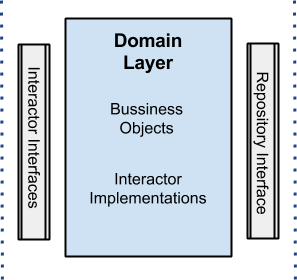
\includegraphics[width=200px]{capitulo5/android/img/capa-dominio.png}
    \caption{Capa de dominio \cite{cleanWay}}
    \label{fig:capa-dominio}
\end{figure}

Para tener un control sobre posibles errores en la capa de presentación o en la capa de datos se utilizan códigos de resultados al igual que una clase que contiene el resultado que se puede presentar, así como la información que se le regresa a la capa de presentación. Se hace uso de genéricos para poder reutilizar esta clase en toda la aplicación y no duplicar código. La clase es la siguiente.

\lstinputlisting[language=Java]{capitulo5/android/src/BusinessResult.java}

La forma en la que se utiliza esta clase en un caso de uso se presenta en el siguiente código que permite iniciar sesión.

\lstinputlisting[language=Java]{capitulo5/android/src/UserInteractorImpl.java}

A su vez el caso de uso utiliza sus propios clases de java para presentar información al usuario en la capa de presentación así como controlar posibles errores en la información que ingrese el usuario los campos de los formularios, un ejemplo de este tipo de clases es el siguiente.

\lstinputlisting[language=Java]{capitulo5/android/src/UsuarioModel.java}

\subsubsection{Capa de presentación}
En esta capa como se muestra en la figura \ref{fig:capa-presentacion} se trabaja con la lógica relacionada a las interfaces que se tienen en la aplicación, es decir a actividades, fragmentos y archivos XML.

\begin{figure}[h]
    \centering
    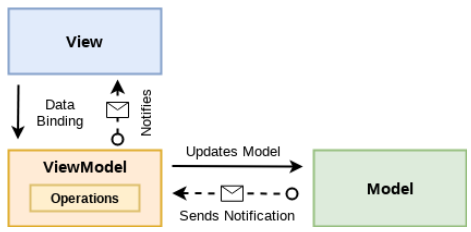
\includegraphics[width=300px]{capitulo5/android/img/capa-presentacion.png}
    \caption{Capa de presentación \cite{cleanWayReload}}
    \label{fig:capa-presentacion}
\end{figure}

En esta capa se pueden trabajar con patrones como MVC y MVP pero en este caso se utiliza el patrón MVVM cada uno con una función en particular. \cite{cleanWayReload}

\begin{itemize}
    \item \textbf{Modelo} Se encarga de representar la información que sera presentada en la vista.
    \item \textbf{Vista} Compuesta en este caso por las actividades y fragmentos de la aplicación, su tarea es mostrar la información, hacen uso de los viewmodels para poder realizar cambios en la interfaz.
    \item \textbf{ViewModel} El ViewModel sera el encargado de ejecutar los casos de uso o interactors con el objetivo de actualizar la vista de acuerdo a la información que presente el modelo.
\end{itemize}



\chapter{Análisis del sistema}

%Todo el análisis previo al diseño y desarrollo del sistema, hasta cierto punto lo más de hueva que se tienen que hacer pero que fundamenta el porque realizar el trabajo. Las secciones que deberiamos cubrir en este apartado son las siguientes:
%
%\begin{itemize}
%    \item Factibilidad
%        \begin{itemize}
%            \item técnica
%            \item operativa
%            \item económica
%            \item analisis de factibilidad (conclusiones con base en los tres puntos anteriores)
%        \end{itemize}
%    \item Requerimientos
%        \begin{itemize}
%            \item funcionales
%            \item no funcionales
%            \item operativos o de sistema
%        \end{itemize}
%    \item Reglas de negocio
%    \item Análisis de riesgos
%    \item Descripción del software
%    \item Herramientas de desarrollo
%    \item Metodología
%\end{itemize}

\section{Requerimientos funcionales}
    Los requerimientos funcionales describen los actividades y comportamientos que tendrá el sistema bajo ciertas condiciones, de igual forma pueden declarar lo que el sistema no debe de hacer.
    
    En esta sección se presentan los requerimientos funcionales que se obtuvieron para el sistema. Dichos requerimientos se encuentran separados de acuerdo a los diferentes módulos que se tienen planeados.
    \subsection{Módulo de usuarios}
    \begin{enumerate}[label=\textbf{RF\arabic*.}]
    \item \textbf{Mecanismo de gestión de usuarios.} Proporcionar al usuario la posibilidad de creación, consulta y modificación de los datos de su cuenta de usuario. Estas operaciones debe de estar presentes en la aplicación web y de android y solo serán permitidas para usuarios con cuenta verificada.
    \item \textbf{Mecanismo de autenticación de usuarios.} Proporcionar un mecanismo para el inicio y cierre de sesión de la cuenta del usuario cuya cuenta haya sido verificada en la aplicación web y android.
    \item \textbf{Mecanismo de verificación de cuenta.} Proporcionar al usuario una forma para verificar que una cuenta creada es valida a través de una verificación basada en el envió de un correo electrónico para la confirmar dicha validez y hacer uso del resto de funcionalidad del sistema. Esta verificación solo se podra realizar a través de la aplicación web.
    \item \textbf{Mecanismo de recuperación de contraseñas.} Proporcionar al usuario la posibilidad de recuperar la contraseña asociada a su cuenta a través de un envío de correo electrónico con el cual podrá acceder a una interfaz en la aplicación web para recuperar el acceso a su cuenta. La recuperación de contraseñas estará disponible en la aplicación android y web.
    \item \textbf{Mecanismo para la comunicación entre la aplicación android y web.} El sistema debe de contar con una interfaz para la comunicación entre las dos aplicaciones que se tienen, la forma en que se realizara sera un API REST y el formato para el envió de información sera JSON.
    \item \textbf{Mecanismo para la autenticación en el API REST.} El sistema debe de brindar una forma de garantizar que la comunicación entre la aplicación web y android es seguro mediante el uso de tokens de autenticación en cada petición y respuesta que se realice.
    \end{enumerate}
    
    \subsection{Módulo de proyectos}
    \begin{enumerate}[label=\textbf{RF\arabic*.}]
    	\setcounter{enumi}{4}
    	\item \textbf{Mecanismo para la gestión de proyectos de \LaTeX{}.} Proporcionar al usuario un mecanismo para visualizar, editar, crear o borrar proyectos asociados a su cuenta. La gestión se podrá realizar en la aplicación web y android.
    	\item \textbf{Permitir descargar el archivo de \LaTeX{}} que se haya traducido. Proporcionar al usuario la funcionalidad de generar un archivo \LaTeX{} que contenga la traducción de expresiones matemáticas que se encuentren en un proyecto. La descarga de dicho archivo solo estará disponible en la aplicación web.
    	\item \textbf{Permitir calificar una traducción realizada.} Proporcionar al usuario la funcionalidad de calificar que tan buena fue la traducción de una expresión matemática en una imagen para brindar retroalimentación, dicha calificación podrán ser valores enteros entre 1 y 5. Para poder calificar una traducción se tendrá que hacer uso de la aplicación web.
    	\item \textbf{Permitir el uso de la cámara del dispositivo android para tomar fotografías.} Proporcionar un mecanismo en la aplicación web que permita acceder a la cámara del dispositivo, tomar una fotografía, visualizarla.
    	\item \textbf{Permitir la visualización del resultado de la traducción.} Proporcionar al usuario una interfaz en la cual pueda observar la traducción a \LaTeX{} que se realizó a partir de una imagen. Esto se podrá hacer en la aplicación web y android.
    	\item \textbf{Permitir añadir al portapapeles alguna traducción seleccionada.} Proporcionar al usuario la funcionalidad para copiar el código de una traducción a su portapapeles para su posterior uso. Esta funcionalidad está limitada a solo la aplicación web.
    	\item \textbf{Mecanismo para el envío de imágenes tomadas por la aplicación android a la aplicación web para su uso.} El sistema debe de tener un mecanismo que a través del uso del API REST permita a la aplicación android el enviar una imagen a la aplicación web para que esta sea tratada. 
    \end{enumerate}
    
    \subsection{Módulo de análisis}
    \begin{enumerate}[label=\textbf{RF\arabic*.}]
    	\setcounter{enumi}{11}
    	\item \textbf{Mecanismo para el tratamiento de la imagen previo a su análisis.} El sistema deberá de realizar un tratamiento al imagen que reciba de la aplicación android para hacer que esta sea más sencilla de trabajar destacando sus partes importantes.
    	\item \textbf{Mecanismo para el reconocimiento de un conjunto definido de expresiones matemáticas en imágenes.} El sistema deberá de reconocer ciertas expresiones en particular con la posibilidad de que expresiones que no se encuentren en este conjunto produzcan resultados no esperados.
    \end{enumerate}
    
    \subsection{Módulo de traducción}
    \begin{enumerate}[label=\textbf{RF\arabic*.}]
    	\setcounter{enumi}{13}
    	\item \textbf{Mecanismo para la traducción a \LaTeX{} de las expresiones matemáticas encontradas en el modulo de análisis.} Implementar un algoritmo basado de gramáticas, redes neuronales o arboles de recubrimiento mínimo que permita transformar la salida que proporcione el módulo de análisis a código \LaTeX que pueda ser interpretado por un compilador.
    \end{enumerate}
    
\section{Requerimientos No Funcionales} 
    A continuación se enlistan los requerimientos no funcionales.
        \begin{enumerate}[label=RNF\arabic*.]
            \item Usabilidad. La interfaz de usuario debe de ser intuitiva con el objetivo de hacer uso de las funcionalidades del sistema de una forma fácil para el usuario.
            
            \item Seguridad. La seguridad se solventa al realizar un cifrado de las contraseñas de los usuarios así como una verificación de la cuenta del usuario para poder hacer uso del sistema. Por otro lado, en la comunicación que se realiza entre la aplicación móvil y el API REST se utiliza un token para autenticar las peticiones que se realizan, dicho token es único para cada usuario. 
            
            \item Escalabilidad. El sistema deberá ser fácilmente escalable y con ello poseer la cualidad de que si se agregan nuevas funcionalidades, estas sean fáciles de acoplar con lo ya desarrollado. Además, de que debe de ser posible aumentar sus capacidades para brindar servicio a más usuarios.
            
            \item Disponibilidad. El sistema debería estar disponible en la mayor parte del tiempo, para lograr esto el uso de un proveedor de hosting es necesario. Entre las posibles opciones están Amazon Web Services, Azure o Google Cloud
            
        \end{enumerate}    
\section{Requerimientos técnicos}
    A continuación se en listan los requerimientos técnicos para un mejor funcionamiento del sistema:
    \subsection{Aplicación móvil}
    \subsubsection{Requerimientos mínimos de software}
    \begin{enumerate}
        \item Sistema operativo Android 4.5 o superior.
        \item Conexión a internet.
    \end{enumerate}
    
    \subsubsection{Requerimientos mínimos de hardware}
    \begin{enumerate}
        %\item Resolución cámara: 13 Megapixeles
        %\item Procesador: Dualcore de 1.2 GHz.
        \item Memoria RAM: 2 GB.
        \item Espacio de almacenamiento de 50 MB.
        \item Cámara de al menos 8 Megapixeles.
    \end{enumerate}
    \subsection{Aplicación web}
    \subsubsection{Requerimientos mínimos de software}
    \begin{enumerate}
        \item Cualquiera de las versiones de los siguientes navegadores hasta su versión más reciente.
        \begin{itemize}
            \item Google Chrome 7
            \item Edge 18
            \item Internet Explorer 11
            \item Firefox 4
            \item Safari 5
            \item Opera 12.1
            \item iOS Safari 13.1
            \item Chrome for android 76
            \item Firefox para android 68
        \end{itemize}
    \end{enumerate}
    \subsubsection{Requerimientos mínimos de hardware}
    \begin{enumerate}
        \item Memoria RAM: 2 GB.
        \item Espacio de almacenamiento de 100 MB.
    \end{enumerate}
    %Poner los recomendados?

\section{Reglas de Negocio}
En esta sección se presentan las reglas de negocio que se necesitan para la elaboración del sistema.
\subsection{RN-001 Campos obligatorios} \label{RN001}
    \begin{enumerate}[label= ]
        %\item Tipo: Derivación. 
        %\item Nivel: Controla la operación.
        \item \textbf{Descripción:} Aquellos campos que son obligatorios no pueden dejarse vacíos.
        \item \textbf{Ejemplo:} Si se tiene un formulario donde existan los siguientes campos:
        \begin{itemize}
            \item Campo 1
            \item Campo 2 (obligatorio)
            \item Campo 3
        \end{itemize}
        El usuario puede dejar los campos 1 y 2 vacíos pero el obligatorio no se podrá omitir.
    \end{enumerate}
    
\subsection{RN-002 Datos correctos} \label{RN002}
    \begin{enumerate}[label= ]
        %\item Tipo: Derivación. 
        %\item Nivel: Controla la operación.
        \item \textbf{Descripción:} Para que los datos sean considerados correctos deben de cumplir con lo establecido en el modelo de información del sistema.
    \end{enumerate}

\subsection{RN-003 Unicidad de identificadores} \label{RN003}
    \begin{enumerate}[label= ]
        %\item Tipo: Restricción. 
        %\item Nivel: Controla la operación.
        \item \textbf{Descripción:} En el conjunto de entidades del sistema, no puede existir elementos con el mismo identificador.
        \item \textbf{Ejemplo de cumplimiento:} Registro de usuario en el cual el correo es el identificador y se puede dar el siguiente caso.
              \begin{itemize}
                  \item Usuario1: \{nombre=Carlos, correo=carlos\_isc7@outlook.com\}
                  \item Usuario2: \{nombre=Juan, correo=gladwell45@outlook.com”\}
              \end{itemize}
        \item \textbf{Ejemplo de fallo:} Registro de usuario en el cual el correo es el identificador y por ende no se puede dar el siguiente caso.
            \begin{itemize}
                \item Usuario1: \{nombre=Ian, correo=carlos\_isc7@outlook.com\}
                \item  Usuario2: \{nombre=Juan, correo=carlos\_isc7@outlook.com\}
            \end{itemize}
    \end{enumerate}

\subsection{RN-004 Calificación proyecto} \label{RN004}
    \begin{enumerate}[label= ]
        %\item Tipo:  
        %\item Nivel: Controla la operación.
        \item \textbf{Descripción:} La calificación de un proyecto tendrá un valor entre 1 y 5 resultado del promedio de las traducciones asociadas a dicho proyecto sin decimales que se hará a través de un redondeo.
        \item \textbf{Sentencia:} Sea: \\
        \[ C_p = \frac{1}{n} \sum_{i=1}^{n} x_i \]
        Donde $C_p$ es la calificación del proyecto, $x_i$ es la calificación de la $i$ traducción y $n$ es el número de traducciones calificadas en el proyecto, deberá actualizarse cada que se agregue o elimine una traducción calificada.
         \item \textbf{Ejemplo:} Si se tiene un proyecto con cinco traducción pero solo tres de ellas tienen calificación se tiene lo siguiente:
         \begin{itemize}
             \item Traducción 1: calificación=4
             \item Traducción 2: Sin calificación
             \item Traducción 3: Sin calificación
             \item Traducción 4: calificación=2
             \item Traducción 5: calificación=5
         \end{itemize}
         La calificación del proyecto sera:
           \[ C_p= \frac{4+3+5}{3} = 4 \]
    \end{enumerate}

\subsection{RN-005 Fecha de modificación} \label{RN005}
    \begin{enumerate}[label= ]
        %\item Tipo: . 
        %\item Nivel: Controla la operación.
        \item \textbf{Descripción:} La fecha de modificación se actualizará cada que se agregue o modifique una traducción al proyecto o que se modifique el proyecto en si la fecha se actualizará con el valor al momento en que se haga la modificación.
       \item \textbf{Ejemplo}. Si se tiene un proyecto con la fecha 2019-05-03 y se realiza una modificación el día 2019-05-20 ahora la fecha de modificación del proyecto será 2019-05-20.
    \end{enumerate}
    
\subsection{RN-006 Usuario verificado} \label{RN006}
    \begin{enumerate}[label= ]
        %\item Tipo: Controladora (Batiz puso esta en una similar) 
        %\item Nivel: Controla la operación.
        \item \textbf{Descripción:} Para que un usuario pueda acceder al sistema su cuenta debe de estar verificada.
    \end{enumerate}
\subsection{RN-007 Información necesaria para descargar un proyecto} \label{RN007}
    \begin{enumerate}[label= ]
        %\item Tipo: Controladora (Batiz puso esta en una similar) 
        %\item Nivel: Controla la operación.
        \item \textbf{Descripción:} Para poder descargar un proyecto es necesario que este cuente con un nombre y al menos una traducción realizada.
    \end{enumerate}
\section{Análisis de Riesgos}
Identificar, clasificar y analizar los riesgos potenciales para el presente Trabajo Terminal, nos permite prevenir las posibles amenazas y probables eventos no deseados así como los daños y consecuencias que estos puedan traer al proyecto. La Tabla \ref{tbl:analisis-riesgos} muestra los resultados de nuestro análisis. \\

\begin{center}
    \begin{longtable}{|J{2.5cm}|J{2cm}|J{5cm}|J{5cm}|}
    
        \hline
        \begin{center}
            \textbf{Área de impacto}
        \end{center}                &
        \begin{center}
            \textbf{Nivel de impacto}
        \end{center}                &
        \begin{center}
            \textbf{Causas} 
        \end{center}                &
        \begin{center}
            \textbf{Métodos para contrarrestar el riesgo}
        \end{center} \\ 
        
        \hline
        Funcionalidad de la aplicación.         &
        \begin{center}
            Alto
        \end{center}                            &
        \begin{itemize}
            \item No obtener un conjunto de entrenamiento lo suficientemente grande para realizar una traducción con pocos errores.
            \item Poca precisión por parte del modelo utilizado.
        \end{itemize}                           &
        Investigar sobre posibles nuevos conjuntos de entrenamiento que la comunidad científica libere. \\
        
        \hline
        Software                                &
        \begin{center}
            Medio
        \end{center}                            &
        \begin{itemize}
            \item Cambios drásticos en las herramientas de desarrollo establecidas para el desarrollo del sistema.
        \end{itemize}                           &
        Seleccionar tecnologías que sean estables y utilizadas en la industria. \\
        
        \hline
        Competitividad de la aplicación         &
        \begin{center}
            Alto
        \end{center}                            &
        \begin{itemize}
            \item El lanzamiento de una aplicación similar por parte de una compañía mucho más grande.
        \end{itemize}                           &
        Seguir incrementando la precisión así como las capacidades del presente proyecto con el fin de que pueda competir en el mercado. \\
        
        \hline
        Confianza del usuario                   &
        \begin{center}
            Alto
        \end{center}                            &
        \begin{itemize}
            \item Insatisfacción por parte del usuario por factores tales como la poca precisión de la traducción.
        \end{itemize}                           &
        Seguir incrementando la precisión. Pedirle retroalimentación directa al usuario final. \\
        
        \hline
        
        \caption{Análisis de riesgos.}
        \label{tbl:analisis-riesgos}
        
    \end{longtable}
\end{center}
\newpage   
\section{Descripción del software}
\subsection{Android}
Android es un sistema operativo para móviles que en la actualidad es desarrollado por Google. Esta principalmente pensado para dispositivos con pantalla táctil como smartphones y tablets. Y que en la actualidad junto con iOS son las principales opciones en cuanto a sistemas operativos para teléfonos móviles. Es por esto que en la Tabla \ref{tbl:comparativa-moviles} se hace una comparativa de las principales características que se tomaron en cuenta para la elección de sistema operativo de dispositivos móviles que se usaría en este trabajo.
\begin{center}
    \begin{longtable}{|J{3cm}|J{5cm}|J{5cm}|}
    \hline
    \textbf{Características} & \textbf{Android} & \textbf{iOS} \\ \hline
    Núcleo & UNIX & UNIX \\ \hline
    Lenguajes de desarrollo & Java, C, C++, Kotlin & Swift, C, C++, Objective-C \\ \hline
    Ambiente de desarrollo & Android Studio, disponible en Windows, Linux y MacOS & Xcode, solo disponible en MacOS \\ \hline
    Complejidad de desarrollo & Medio complejo debido a la gran cantidad de diferencias entre dispositivos y versiones de sistema operativo & Poco compleja debido a que hay poca diversidad de versiones sistemas operativos y dispositivos \\ \hline
    Tiempo de desarrollo & Suele tomar 30\%-40\% más que para iOS \cite{ddi} & Depende de la complejidad del desarrollo \\ \hline
    Tiempo de despliegue & Es rápido desplegar una aplicación de Android debido a los test automáticos que se realizan sobre esta para su verificación & Es lento su despliegue debido a que la verificación es manual \\ \hline
    Cantidad del mercado & La cantidad de usuarios es mayor, tan solo el primer cuarto del 2017 el 86.1\% de los teléfonos vendidos fueron Android \cite{ddi} & Su mercado es menor al de Android \\ \hline
    Código abierto & El kernel, UI y algunas aplicaciones estándar son de código abierto & El kernel no es de código abierto pero esta basado en Darwin OS que es de código abierto \\ \hline
    Ultima versión & Android 10 (Septiembre 3, 2019) & iOS 13 (Septiembre 19, 2019) \\ \hline
    Seguridad & Actualizaciones de seguridad bastante regulares. Sin embargo, debido a los fabricantes dichas actualizaciones pueden demorarse en ser aplicadas. También se pueden instalar aplicaciones externas a la Play Store por lo que esto puede generar problemas de seguridad & Pocas actualizaciones, las amenazas de seguridad son pocas debido a que descargar aplicaciones fuera de la App Store es complicado. \\ \hline
    \caption{Tabla comparativa de sistemas operativos de dispositivos móviles}
    \label{tbl:comparativa-moviles}
    \end{longtable}
\end{center}

Android nos brinda un ambiente de desarrollo más flexible que el que presenta iOS debido a las características listadas con anterioridad. Es cierto que el desarrollo puede ser más tardado sin embargo para este proyecto el optar por iOS nos generaría problemas debido a que no solo la plataforma de desarrollo es más cerrada sino que el tiempo de desarrollo seria mayor debido a la curva de aprendizaje de Swift y Objective-C a la cual nos enfrentaríamos.

Finalmente, la cantidad del mercado que tiene Android es significativamente mayor que la que tiene iOS por ende este es un gran punto a considerar. Es por todas estas cuestiones que se opto por desarrollar el trabajo para la plataforma de Android.
\subsection{Base de datos}

Un Sistema Gestor de Bases de Datos (SGBD) o DGBA (Data Base Management System) es un conjunto de programas no visibles que administran y gestionan la información que contiene una base de datos. Para el caso del presente Trabajo Terminal, se decidio utilizar una base de datos relacional. La Tabla \ref{tbl:analisis-bases} muestra una comparativa de los tres principales gestores de bases de datos \cite{basesComparacion}.

\begin{center}
    \begin{longtable}{|m{3.5cm}|m{3.5cm}|m{3.5cm}|m{3.5cm}|}
    
    \hline
    \begin{center}
        \textbf{Características}
    \end{center}                &
    \begin{center}
        \textbf{MySQL}
    \end{center}                &
    \begin{center}
        \textbf{Oracle}
    \end{center}                &
    \begin{center}
        \textbf{PostgreSQL}
    \end{center} \\
    
    \hline
    Modelo de base de datos primario    &
    Relacional                          &
    Relacional                          &
    Relacional  \\
    
    \hline
    Modelo de base de datos secundario  &
    Documento                           &
    Documento, gráfo, RDF               &
    Documento \\
    
    \hline
    Distribución                        &
    Código abierto                      &
    Comercial                           &
    Código abierto \\
    
    \hline
    Implementación                      &
    C y C++                             &
    C y C++                             &
    C \\
    
    \hline
    Sistemas operativos soportados           &
    FreeBSD, Linux, OS X, Solaris y Windows. &
    AIX, HP-UX, Linux, OS X, Solaris, 
    Windows y z/OS.                          &
    FreeBSD, HP-UX, Linux, NetBSD, 
    OpenBSD, OS X, Solaris, Unix, Windows. \\
    
    \hline
    Soporte de XML                      &
    Si                                  &
    Si                                  &
    Si \\
    
    \hline
    Scripts del lado del servidor       &
    Si                                  &
    PL/SQL                              &
    Funciones definidas por el usuario. \\
    
    \hline
    Triggers                            &
    Si                                  &
    Si                                  &
    Si \\
    
    \hline
    Transacciones                       &
    ACID                                &
    ACID                                &
    ACID \\
    
    \hline
    
    \caption{Comparación de diferentes gestores de bases de datos.}
    \label{tbl:analisis-bases}
    
    \end{longtable}
\end{center}

Para el desarrollo del presente proyecto, se selecciono PostgreSQL como gestor de bases de datos, debido a que es de código abierto y contiene más funcionalidades avanzadas de lo que MySQL soporta.




\subsection{Framework de desarrollo web}

Un framework de desarrollo es un conjunto de utilerías y funciones que permiten de una manera consistente acelerar el proceso de creación de una aplicación web. La Tabla \ref{tbl:analisis-frameworks} muestra una comparativa entre los principales frameworks en la industria \cite{fComparacion}.

\begin{center}
    \begin{longtable}{|m{3.5cm}|m{3.5cm}|m{3.5cm}|m{3.5cm}|}
    
    \hline
    \begin{center}
        \textbf{Características}
    \end{center}                &
    \begin{center}
        \textbf{Django}
    \end{center}                &
    \begin{center}
        \textbf{Ruby on Rails}
    \end{center}                &
    \begin{center}
        \textbf{Laravel}
    \end{center} \\
    
    \hline
    Lenguaje soportado          &
    Python                      &
    Ruby                        &
    PHP \\
    
    \hline
    Mercado                     &
    1,192 compañías lo utilizan &
    2,723 compañías lo utilizan &
    1,032 compañías lo utilizan \\
    
    \hline
    Ecosistema                  &
    Muchos paquetes disponibles, entre las más importantes se encuentran: Django REST Framework, Django allauth para la autenticación con redes sociales y Celery.  &
    Cientos de gemas disponibles, librerias como Action Mailer y Active Storage, frameworks como Active Job y Action Cable. &
    Se compone de mas de 15k paquetes. Los más populares son: Cashier, Envoy and Passport, Scout, Socialite, Envoyer, Forge, Horizon, Lumen, entre otros. \\
    
    \hline
    Desempeño                   &
    Respuestas rápidas de texto plano, actualizaciones de la BD eficientes, excelente en la serialización de JSON.      &
    Respuestas buenas de texto plano, eficiente en las actualizaciones de la DB, eficiente respuesta en JSON.  &
    Respuestas buenas de texto plano, excelente en las actualizaciones de la DB. \\
    
    \hline
    Seguridad                                           &
    Provee métodos contra inyección SQL, ataques XSS, CSRF y \textit{clickjacking}. Excelente en el manejo de autenticación de usuarios y permisos. Actualizaciones constantes. &
    Provee métodos contra inyección SQL, ataques XSS, CSRF y \textit{clickjacking}.                              &
    Es vulnerable a ataques, provee métodos de autenticación y hashing. \\
    
    \hline
    \caption{Comparación de frameworks de desarrollo web.}
    \label{tbl:analisis-frameworks}
    
    \end{longtable}
\end{center}

Para el desarrollo de la parte web del presente proyecto, se eligió Django como framework de desarrollo debido a que esta enteramente desarrollado en python, lo que nos permite el uso de las mejores librerias de deep learning, las cuales solo estan soportadas en este lenguaje. Además, Django provee de un conjunto muy robusto de métodos para mantener segura la información.


\section{Traducción de imágenes a \LaTeX}

El problema de traducir imágenes a \LaTeX automáticamente, es aún un campo de investigación abierto. Dada su naturaleza recursiva miltinivel, las inmensas ambigüedades en la escritura y su fuerte dependencia a un contexto claro, esta tarea difiere en gran medida del reconocimiento óptico de caracteres (OCR) para el cual ya existen sistemas con una precisión suficiente. \\

Según \cite{chino}, el reconocimiento de expresiones matemáticas a mano (HMER) comprende dos grandes problemas: reconocimiento de los símbolos y el análisis de su estructura. Existen dos grandes aproximaciones, las cuales son: secuenciales y globales. \\

Las aproximaciones secuenciales, buscan primero reconocer los símbolos y después realizán el análisis estructural por separado. Uno de los problemas que esta aproximación presenta, es que los errores cometidos en la parte del reconocimiento, serán heredados por el análisis estructural, generando una cadena de malas traducciones. La solución secuencial que mejores resultados ha dado, es el uso de grámaticas predefinidas para llevar a cabo el reconocimiento de la estructura de la expresión. \\

La segunda alternativa, combina los dos tipos de análisis en uno solo, pues busca ir reconociendo la estructura a la vez que se reconocen los símbolos. Esta aproximación permite generar la segmentación de símbolos utilizando toda la información disponible de la imagen, por lo que este tipo de soluciones parecen ser una mejor opción, sin embargo, este procedimiento es más costoso computacionalmente. Recientes investigaciones, han utilizado las arquitecturas encoder-decoder mencionadas previamente en el Marco Teórico para atacar el problema de forma global como si fuera una tarea de Image Captioning. Los resultados obtenidos por este tipo de aproximación resultan ser menos costos y más precisos. \\

Las dos propuestas principales, es decir, las gramáticas y la arquitectura encoder-decoder tienen sus limitaciones. En el caso de las gramáticas, podemos ver que los algoritmos para el procesamiento de las mismas incrementan su complejidad exponencialmente entre más expresiones son capaces de reconocer, además de que requieren un conocimiento previo de los símbolos. Mientras que con el avance de los procesadores y GPUs las aproximaciones globales con redes neuronales se vuelven cada vez más plausibles y es por esta razón que los investigadores en el campo del machine learning le han prestado particular atención mejorando así, los resultados obtenidos por cualquier otro método. \\

En el presente Trabajo Terminal, se ha decidido utilizar la aproximación global propuesta por \cite{chino}, la cual es llamada Watch, Attend, Parse (WAP) que es una RNN encoder-decoder con un sistema de atención que permite reconocer expresiones matemáticas escritas a mano con una precisión del 46.55\%. En la Figura \ref{fig:wap} podemos ver un diagrama de esta arquitectura.\\

\begin{figure}[H]
	\centering
	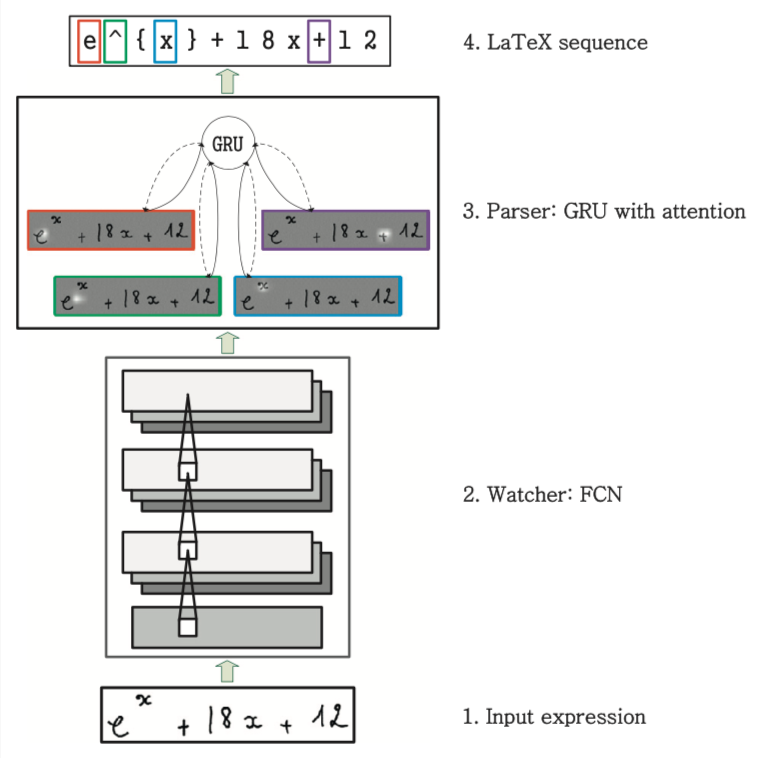
\includegraphics[]{capitulo3/imgs/wap}
	\caption{Diagrama de la arquitectura Watch, Attend, Parse (WAP).}
	\label{fig:wap}
\end{figure}

La red WAP, se compone de dos partes:

\begin{enumerate}
	\item \textbf{Encoder}: El cual es una CNN que permite extraer las características de la imagen y sumarizarlas en un vector de contexto $C$.
	\item  \textbf{Decoder}: El cual es una LSTM que toma el contexto $C$ y junto con sistema de atención retorna como salida la secuencia de símbolos de \LaTeX, un símbolo a la vez.
\end{enumerate}


\newpage
\section{Delimitación de expresiones matemáticas}
\label{sec:del_exp}
Debido a la elección de un modelo sequence to sequence para resolver el problema de reconocimiento y traducción de las expresiones, los símbolos y tipo de expresiones matemáticas a reconocer están limitadas por el conjunto de entrenamiento a utilizar. El presente Trabajo Terminal, se enfocará en reconocer expresiones matemáticas escritas a mano.

La Competición en el Reconocimiento de Expresiones Matemáticas Escritas a Mano \textit{CROHME} de sus siglas en inglés, provee de un conjunto de entrenamiento que consta de casi 10,000 imágenes seperadas en conjuntos de entrenamiento, validación y prueba. Este conjunto de entrenamiento, será el principal conjunto utilizado por el presente Trabajo Terminal.

Existe otro conjunto sobre expresiones matemáticas, fue publicado por \cite{harvard}, se compone cerca de 100,000 imágenes de expresiones matemáticas renderizadas a computadora. Este conjunto solo será utilizado para comprobar como distintos conjuntos de entrenamiento pueden afectar el desempeño del modelo, pues las expresiones renderizadas por computadora, son sustancialmente diferentes de las provistas por CROHME.

Al utilizar el conjunto de entrenamiento CROHME \cite{CROHME} se tomó un análisis de símbolos existentes en dicho conjunto de entrenamiento realizado con ayuda de la herramienta \textbf{CROHME Data Extractor} \cite{EXTRACTOR}. El conteo de apariciones de símbolos arroja las siguientes gráficas de frecuencias clasificando los tipos de símbolos.\\

La primer gráfica muestra la frecuencia de los dígitos del sistema arábigo, donde podemos ver que el dígito \textbf{1} aparece nueve mil cuatrocientos sesenta veces siendo este el de mayor aparición en esta categoría, mientras que el 7 aparece mil veinticinco veces.
\begin{figure}[H]
	\centering
	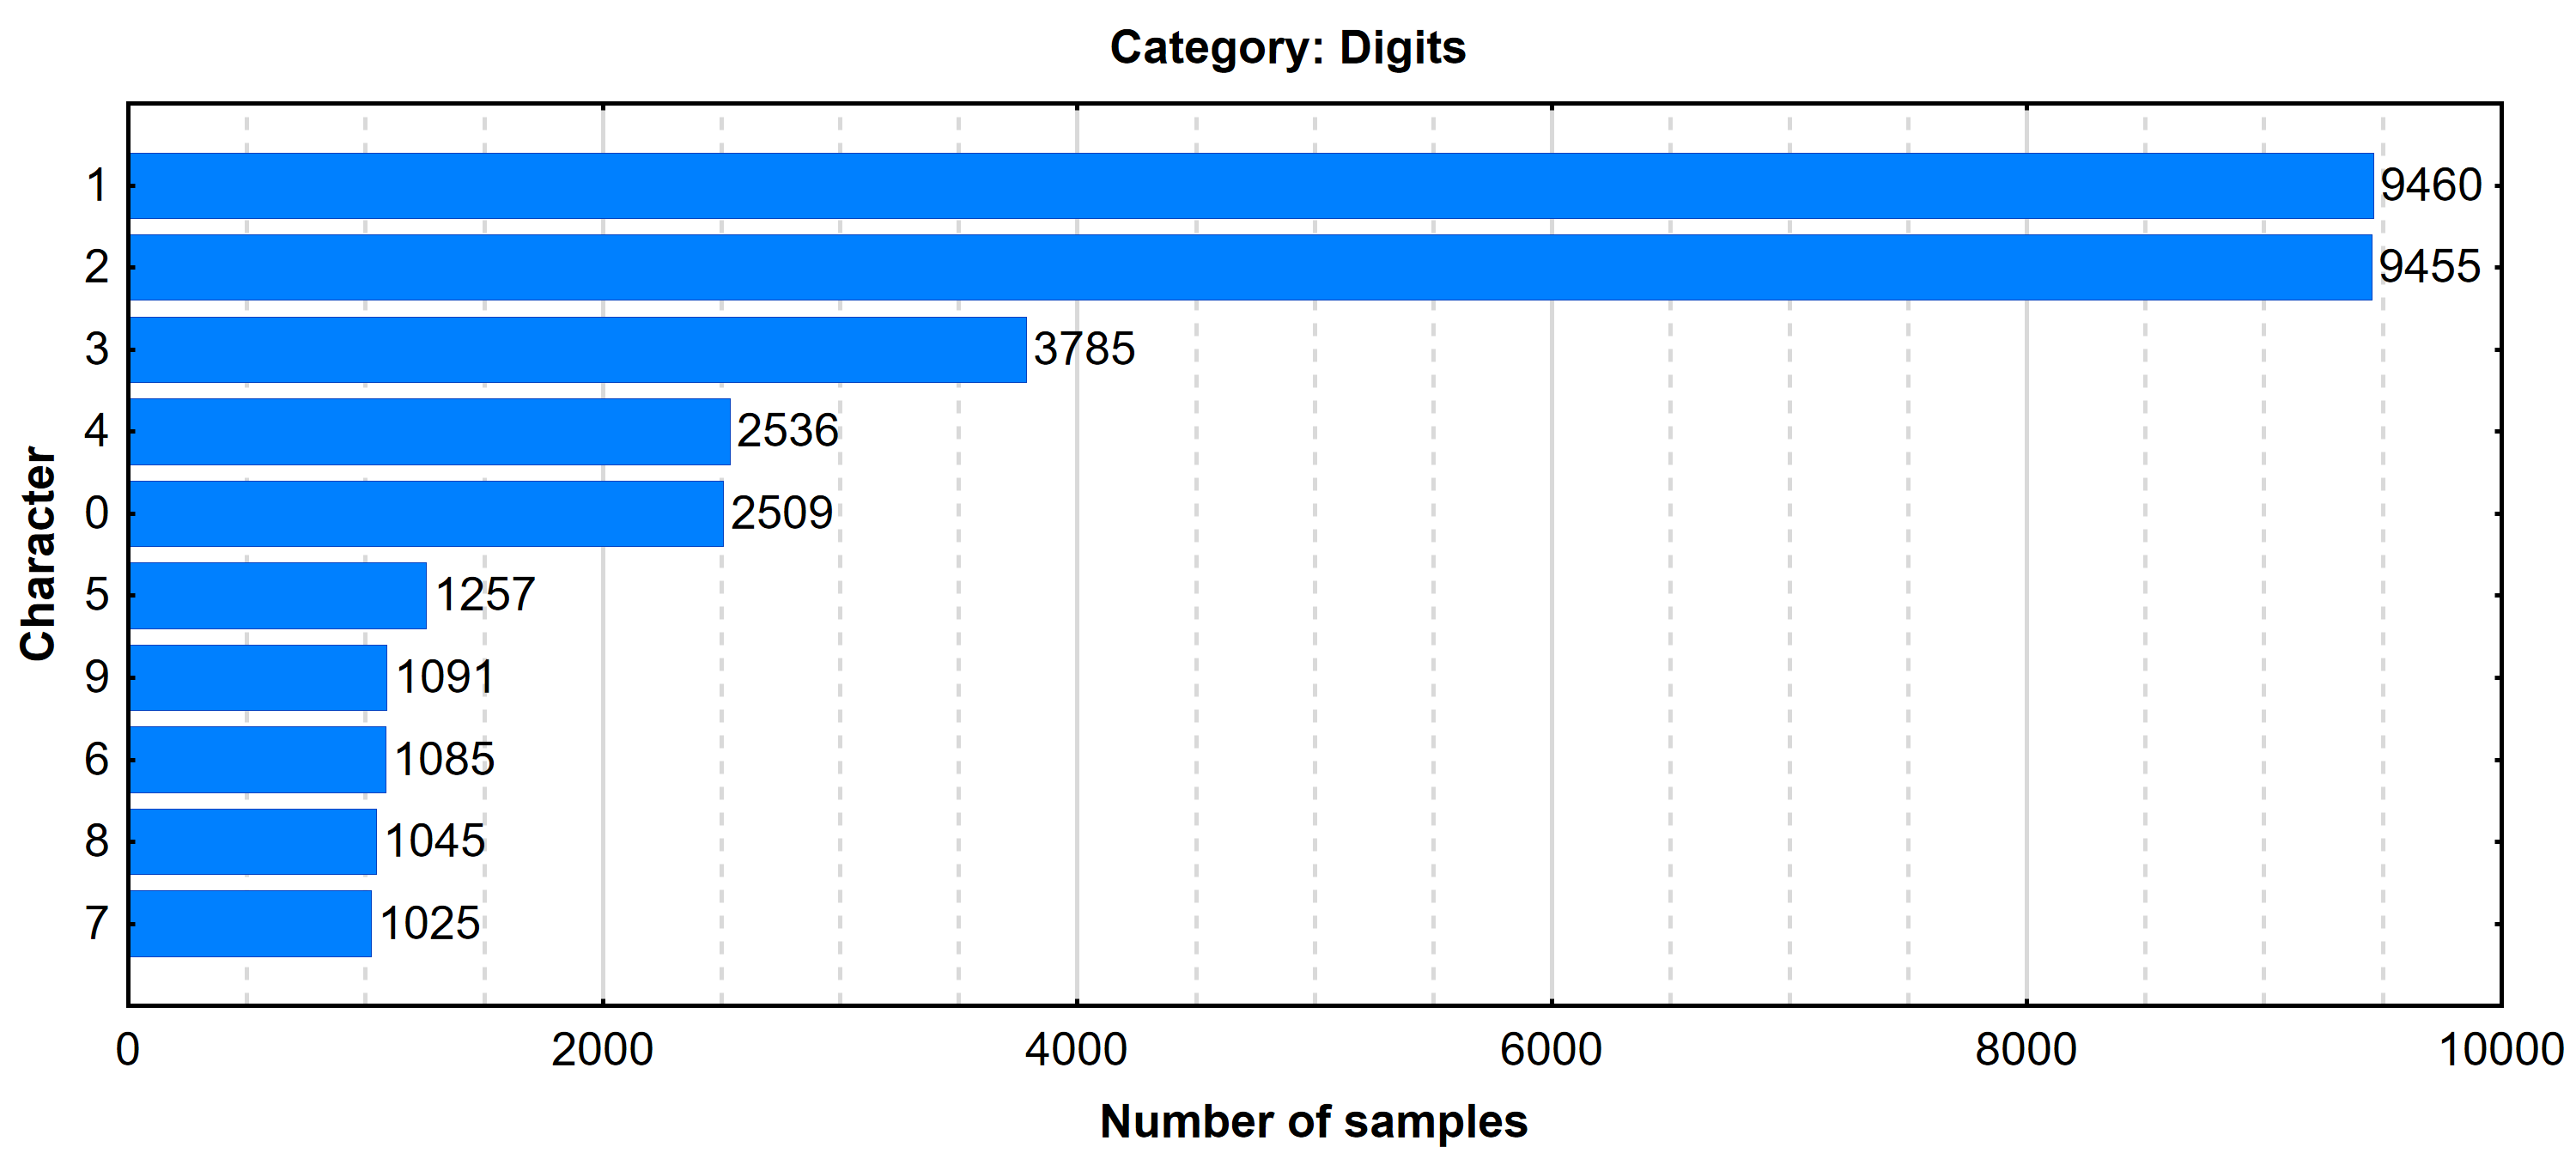
\includegraphics[width=1\textwidth]{capitulo3/imgs/digits_distribution.png}
	\caption{Frecuencia de aparición de dígitos del sistema de numeración arábigo \cite{EXTRACTOR}}
	\label{fig:DigDist}
\end{figure}
\newpage
En el caso de los símbolos matemáticos el de mayor aparición es el símbolo \textbf{-} con doce mil trecientas veintiocho veces. En esta gráfica podemos observar la aparición de símbolos que soportan expresiones que involucren divisiones o funciones trigonométricas o comparadores, incluso cuantificador de existencia aunque con una muy baja frecuencia de tan solo once apariciones.
\begin{figure}[H]
	\centering
	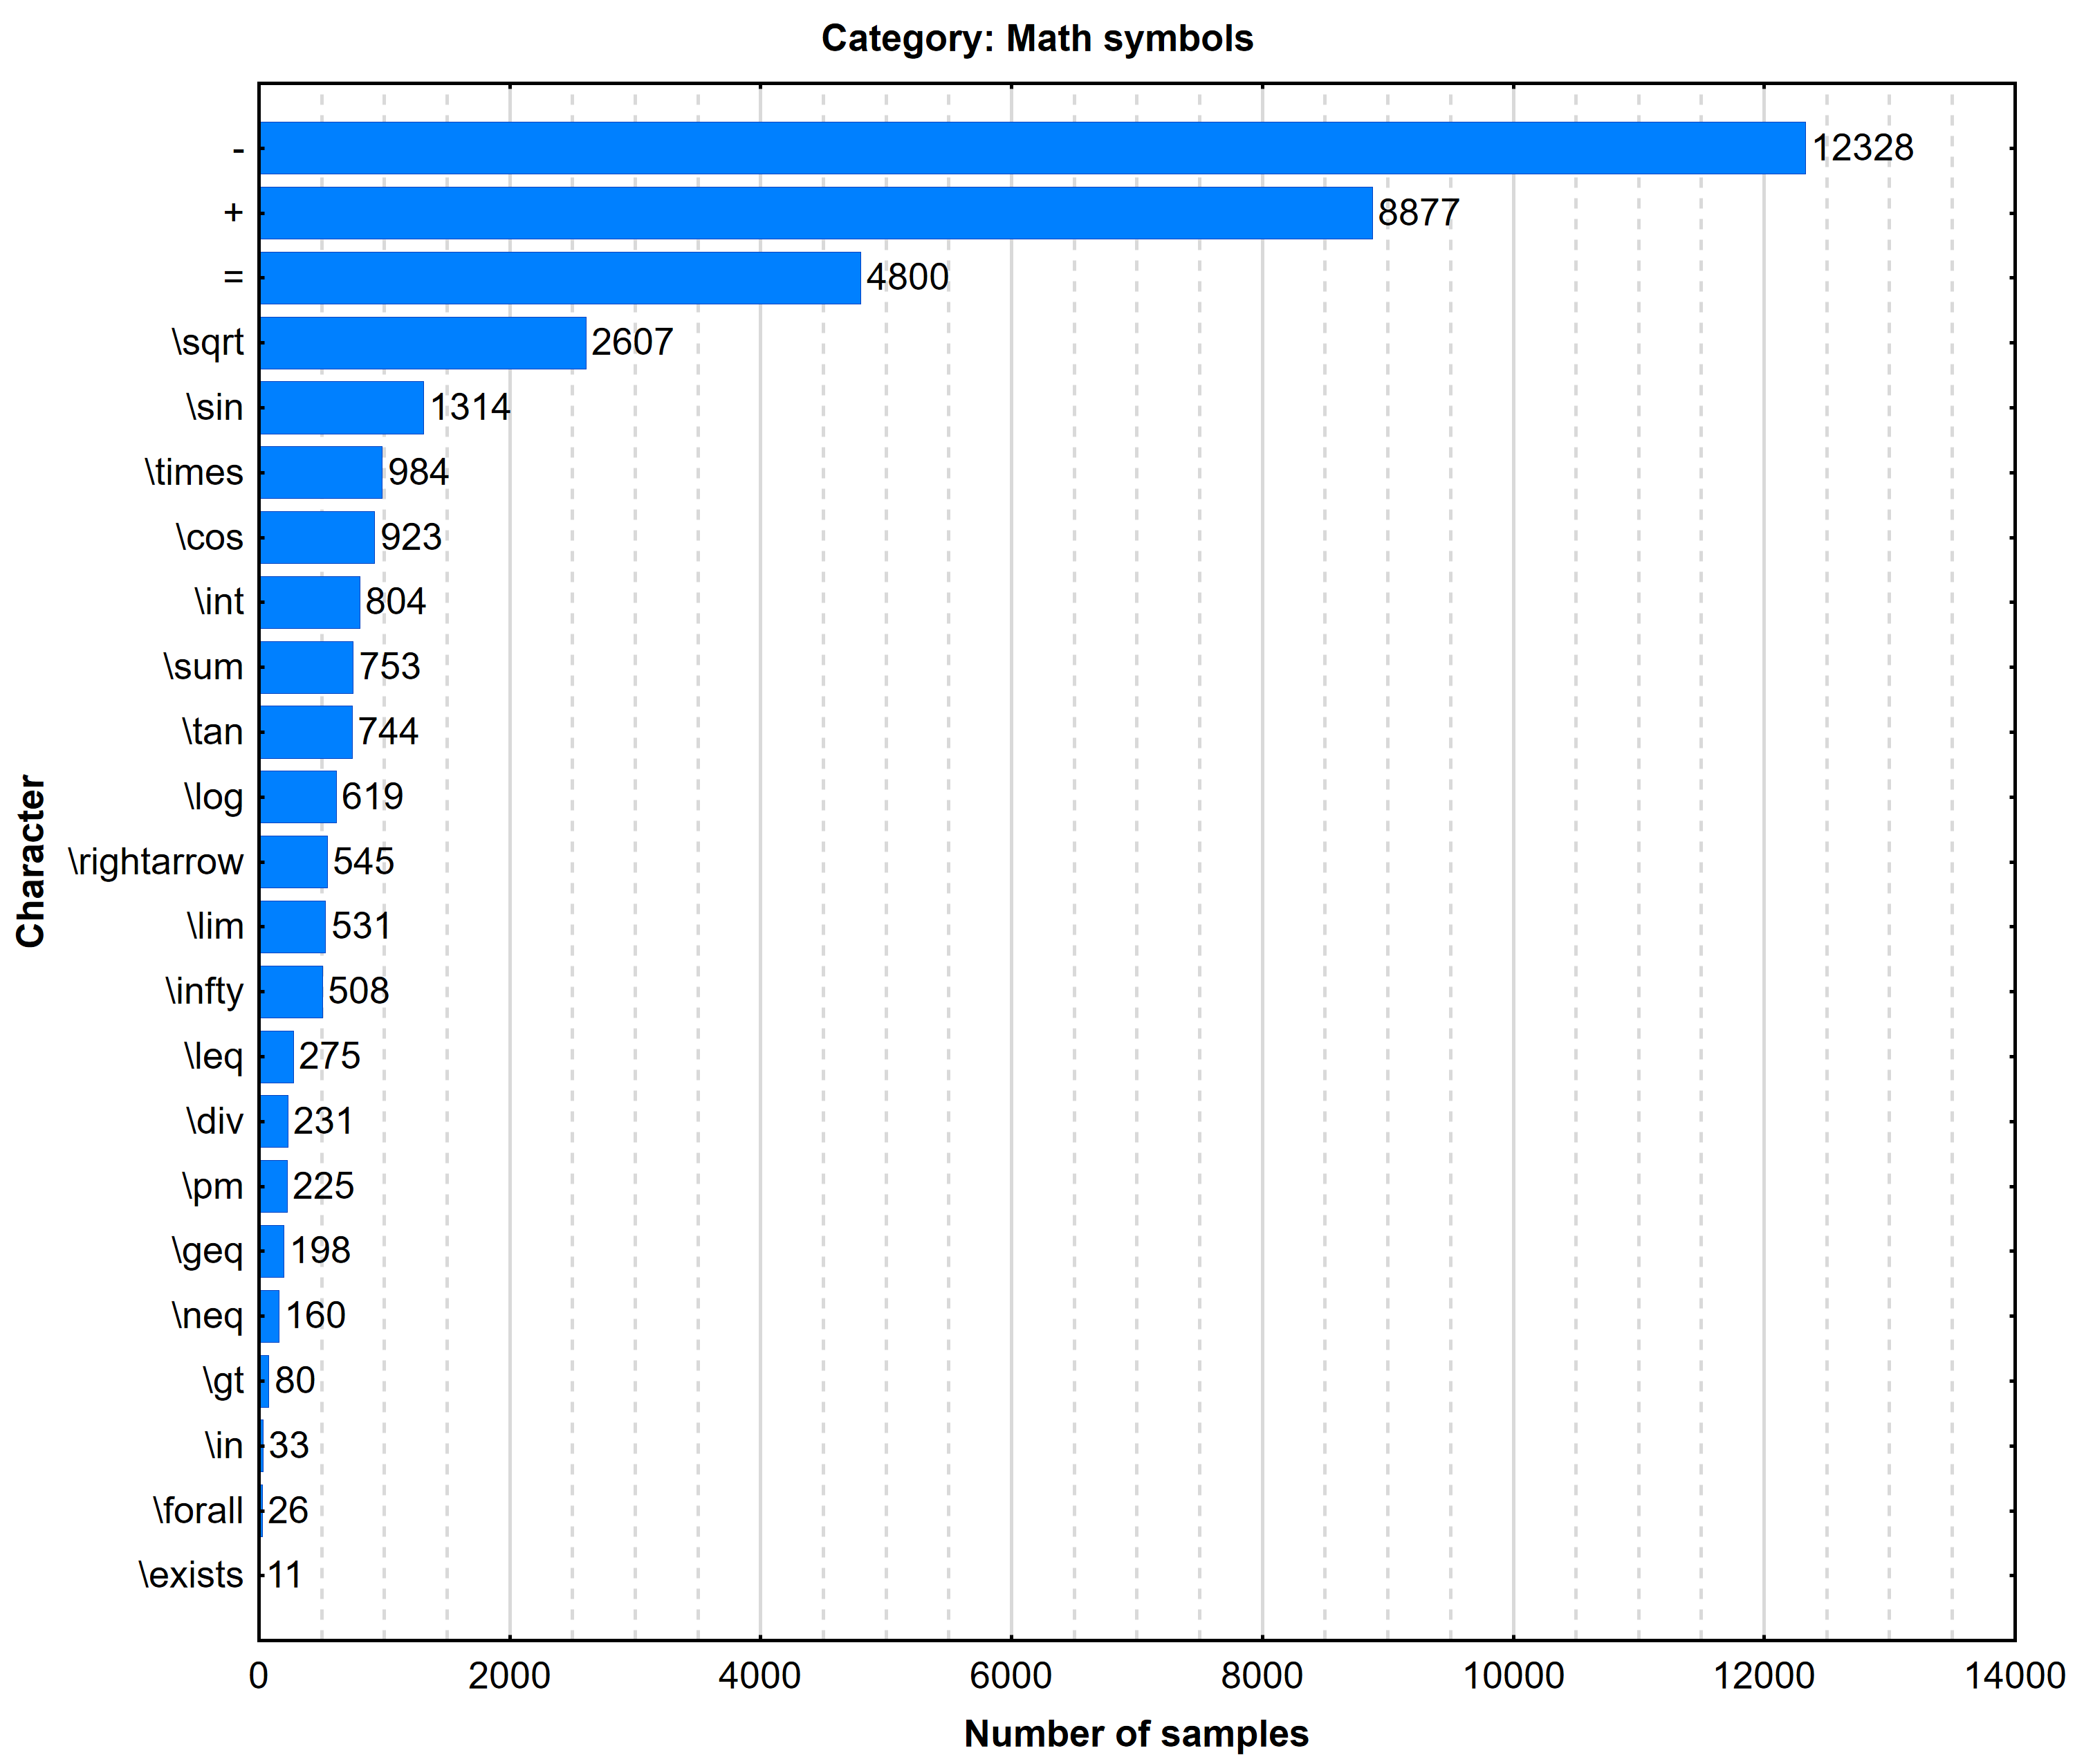
\includegraphics[width=1\textwidth]{capitulo3/imgs/math_symbols_distribution.png}
	\caption{Frecuencia de aparición de símbolos matemáticos \cite{EXTRACTOR}}
	\label{fig:MathSymbols}
\end{figure}
\newpage

En el caso de letras mayúsculas se logró identificar una frecuencia de cuatrocientos sesenta y nueve para el caso de la letra \textbf{C} mientras que para la letra \textbf{I} de noventa y seis.
\begin{figure}[H]
	\centering
	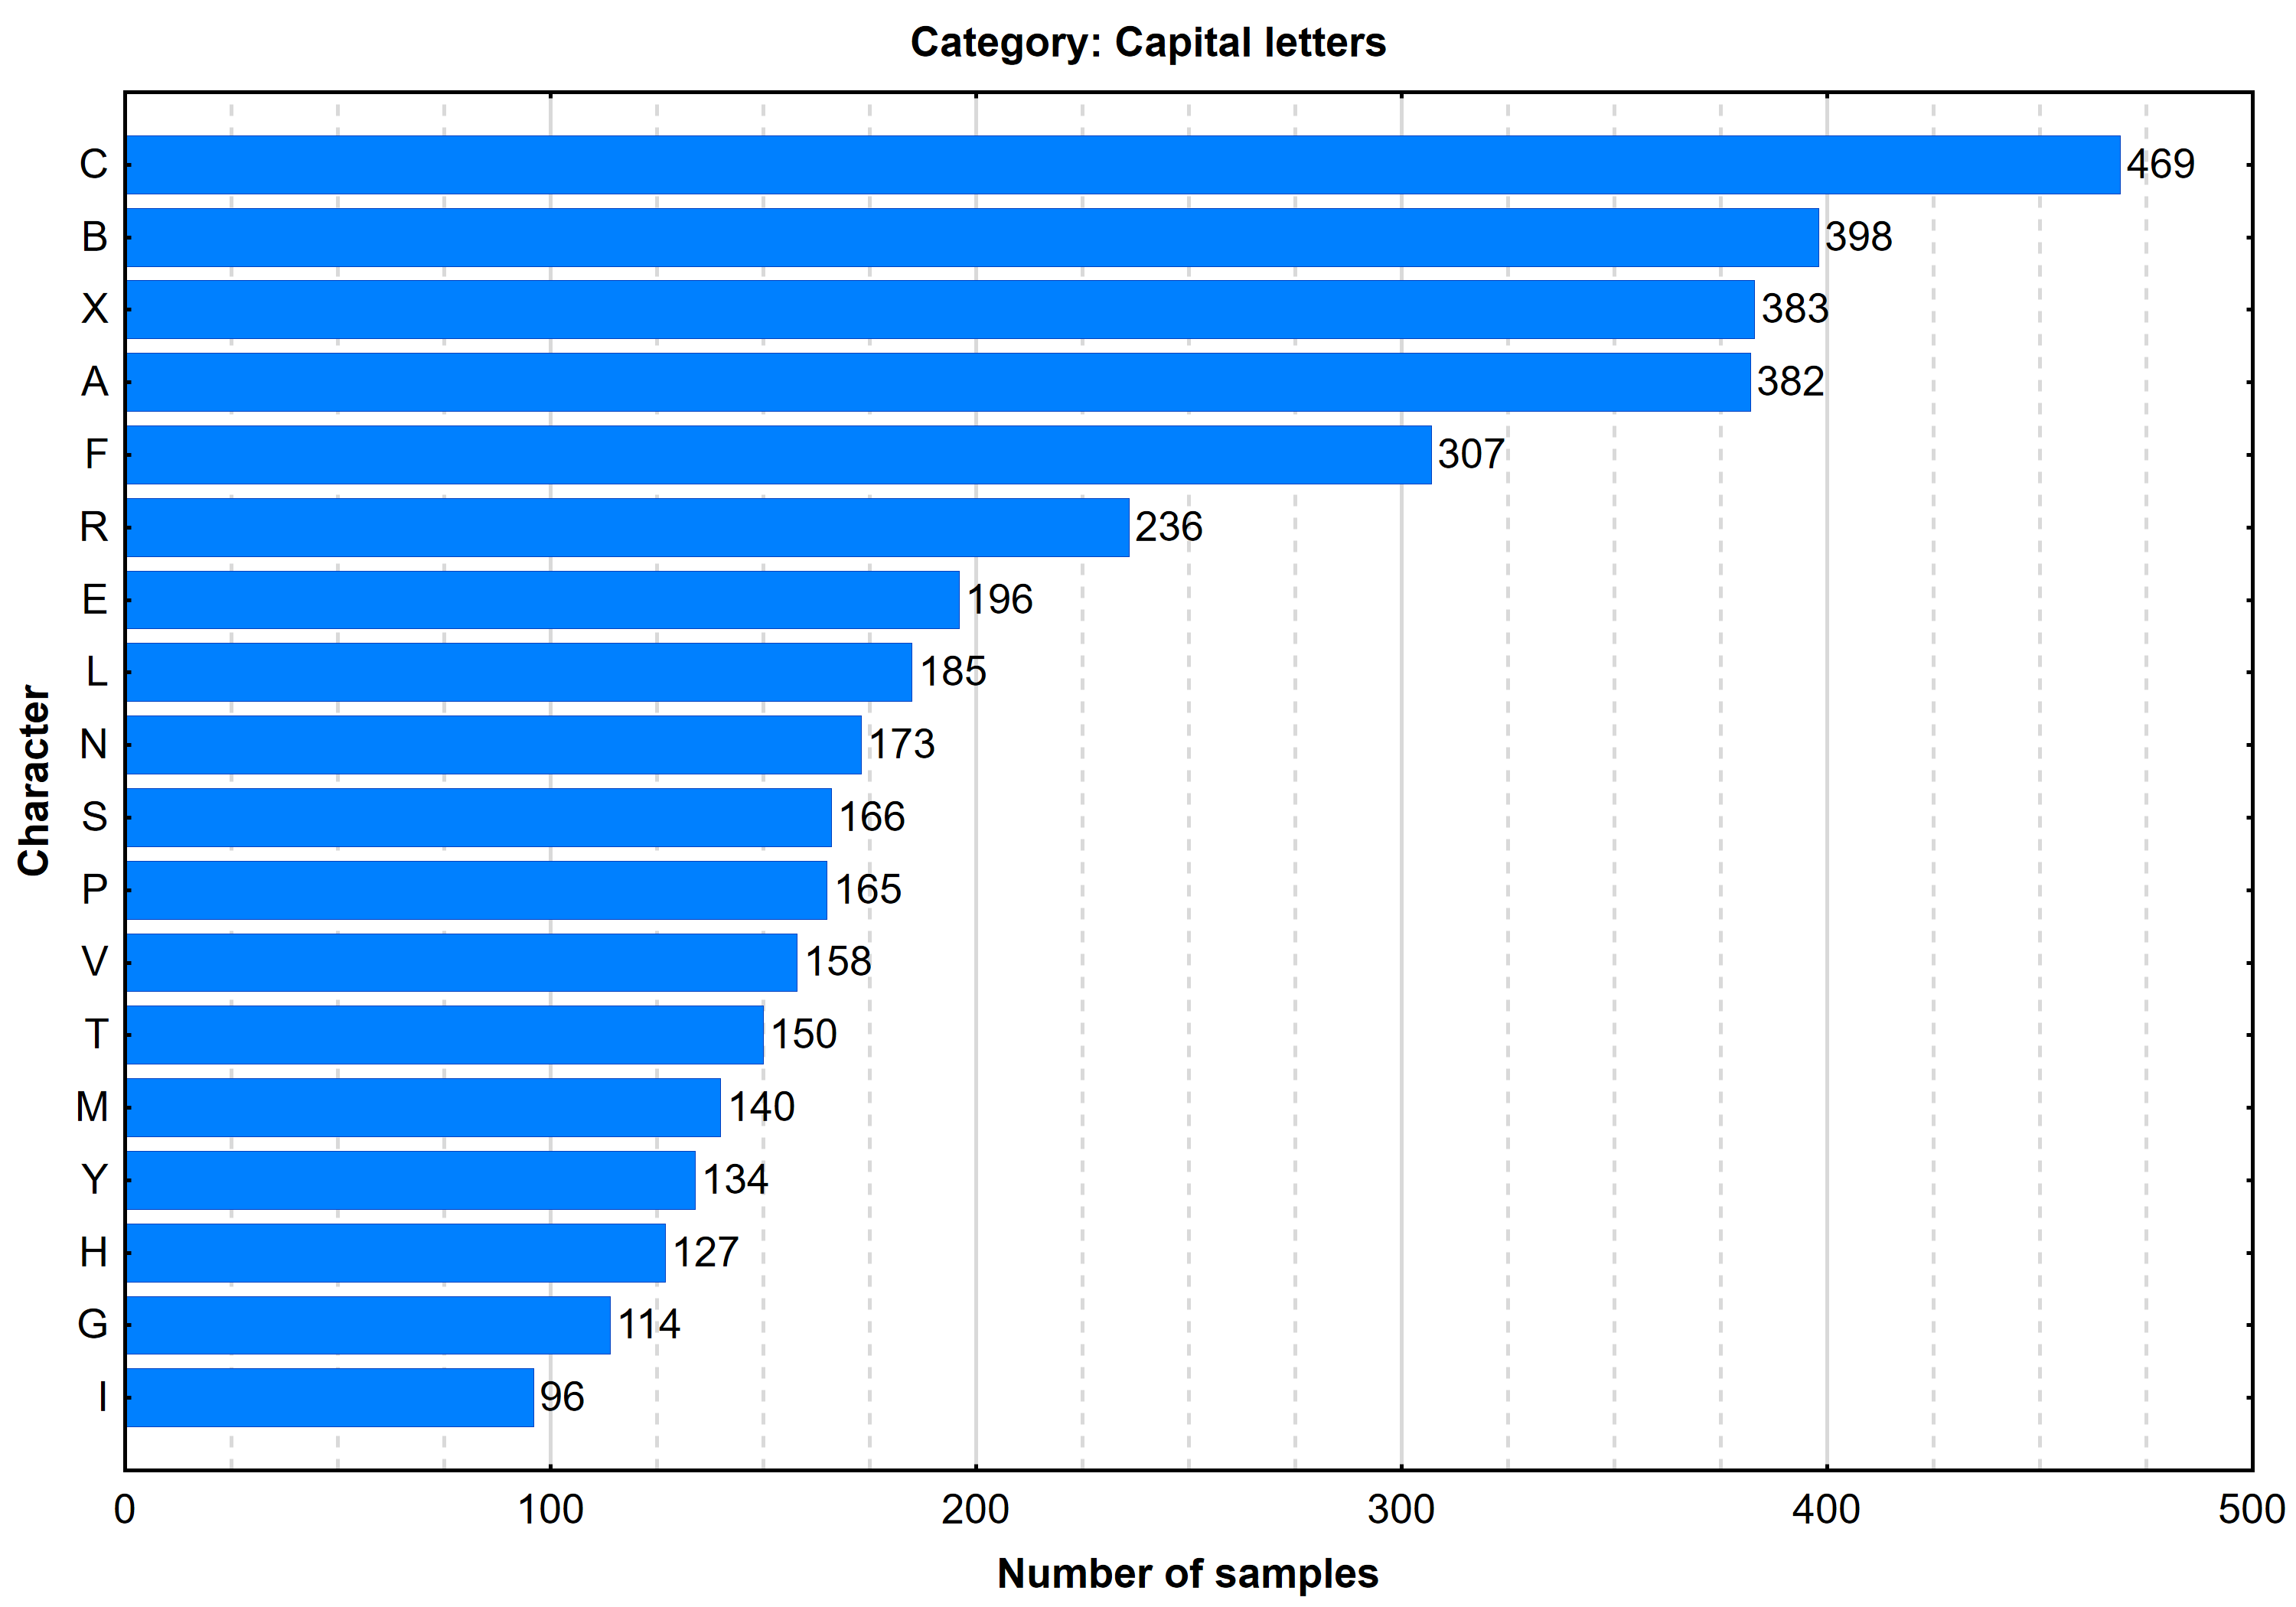
\includegraphics[width=1\textwidth]{capitulo3/imgs/capital_letters_distribution.png}
	\caption{Frecuencia de aparición de letras mayúsculas \cite{EXTRACTOR}}
	\label{fig:CapLetters}
\end{figure}
\newpage
En el caso de las letras minúsculas como podría esperarse la letra $\textbf{x}$ tiene la mayor aparición con ocho mil ciento nueve veces.
\begin{figure}[H]
	\centering
	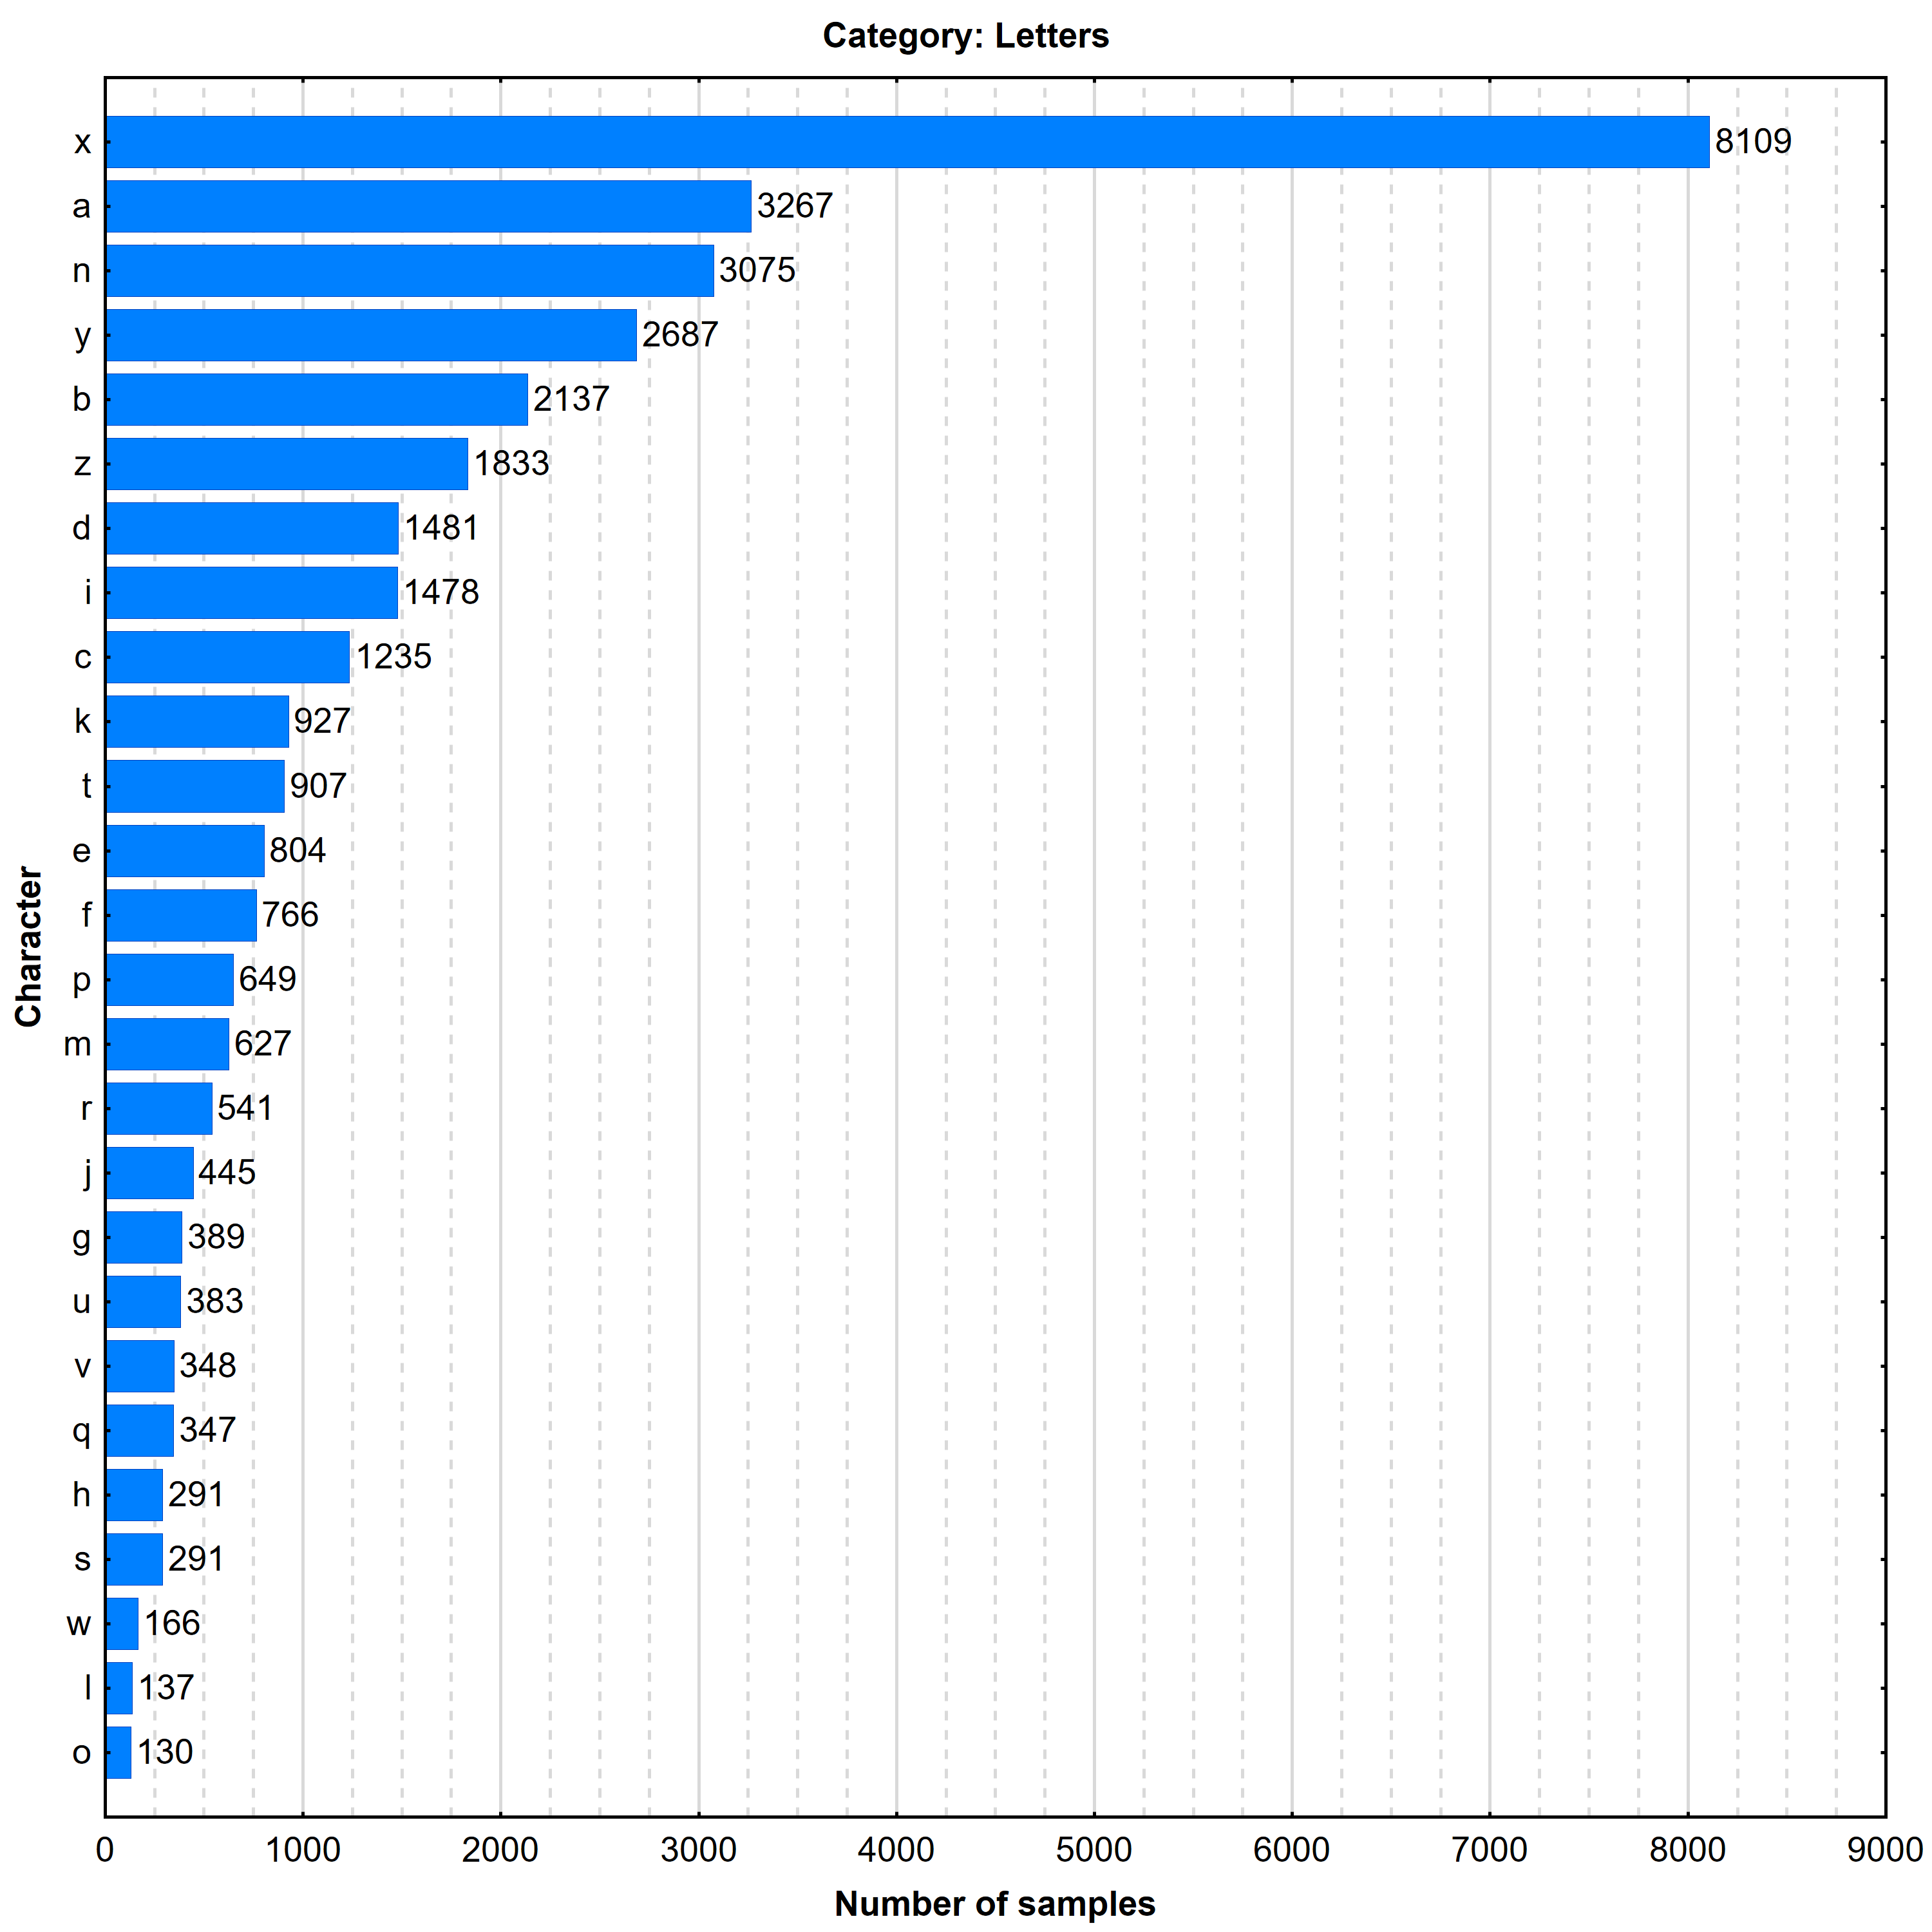
\includegraphics[width=1\textwidth]{capitulo3/imgs/lowercase_letters_distribution.png}
	\caption{Frecuencia de aparición de letras minúsculas \cite{EXTRACTOR}}
	\label{fig:LowerLetters}
\end{figure}
\newpage
La categoría con menos elementos pertenece a las letras griegas con nueve caracteres, siendo $\alpha$ (alpha) el de mayor aparición con ochocientas diecinueve veces.
\begin{figure}[H]
	\centering
	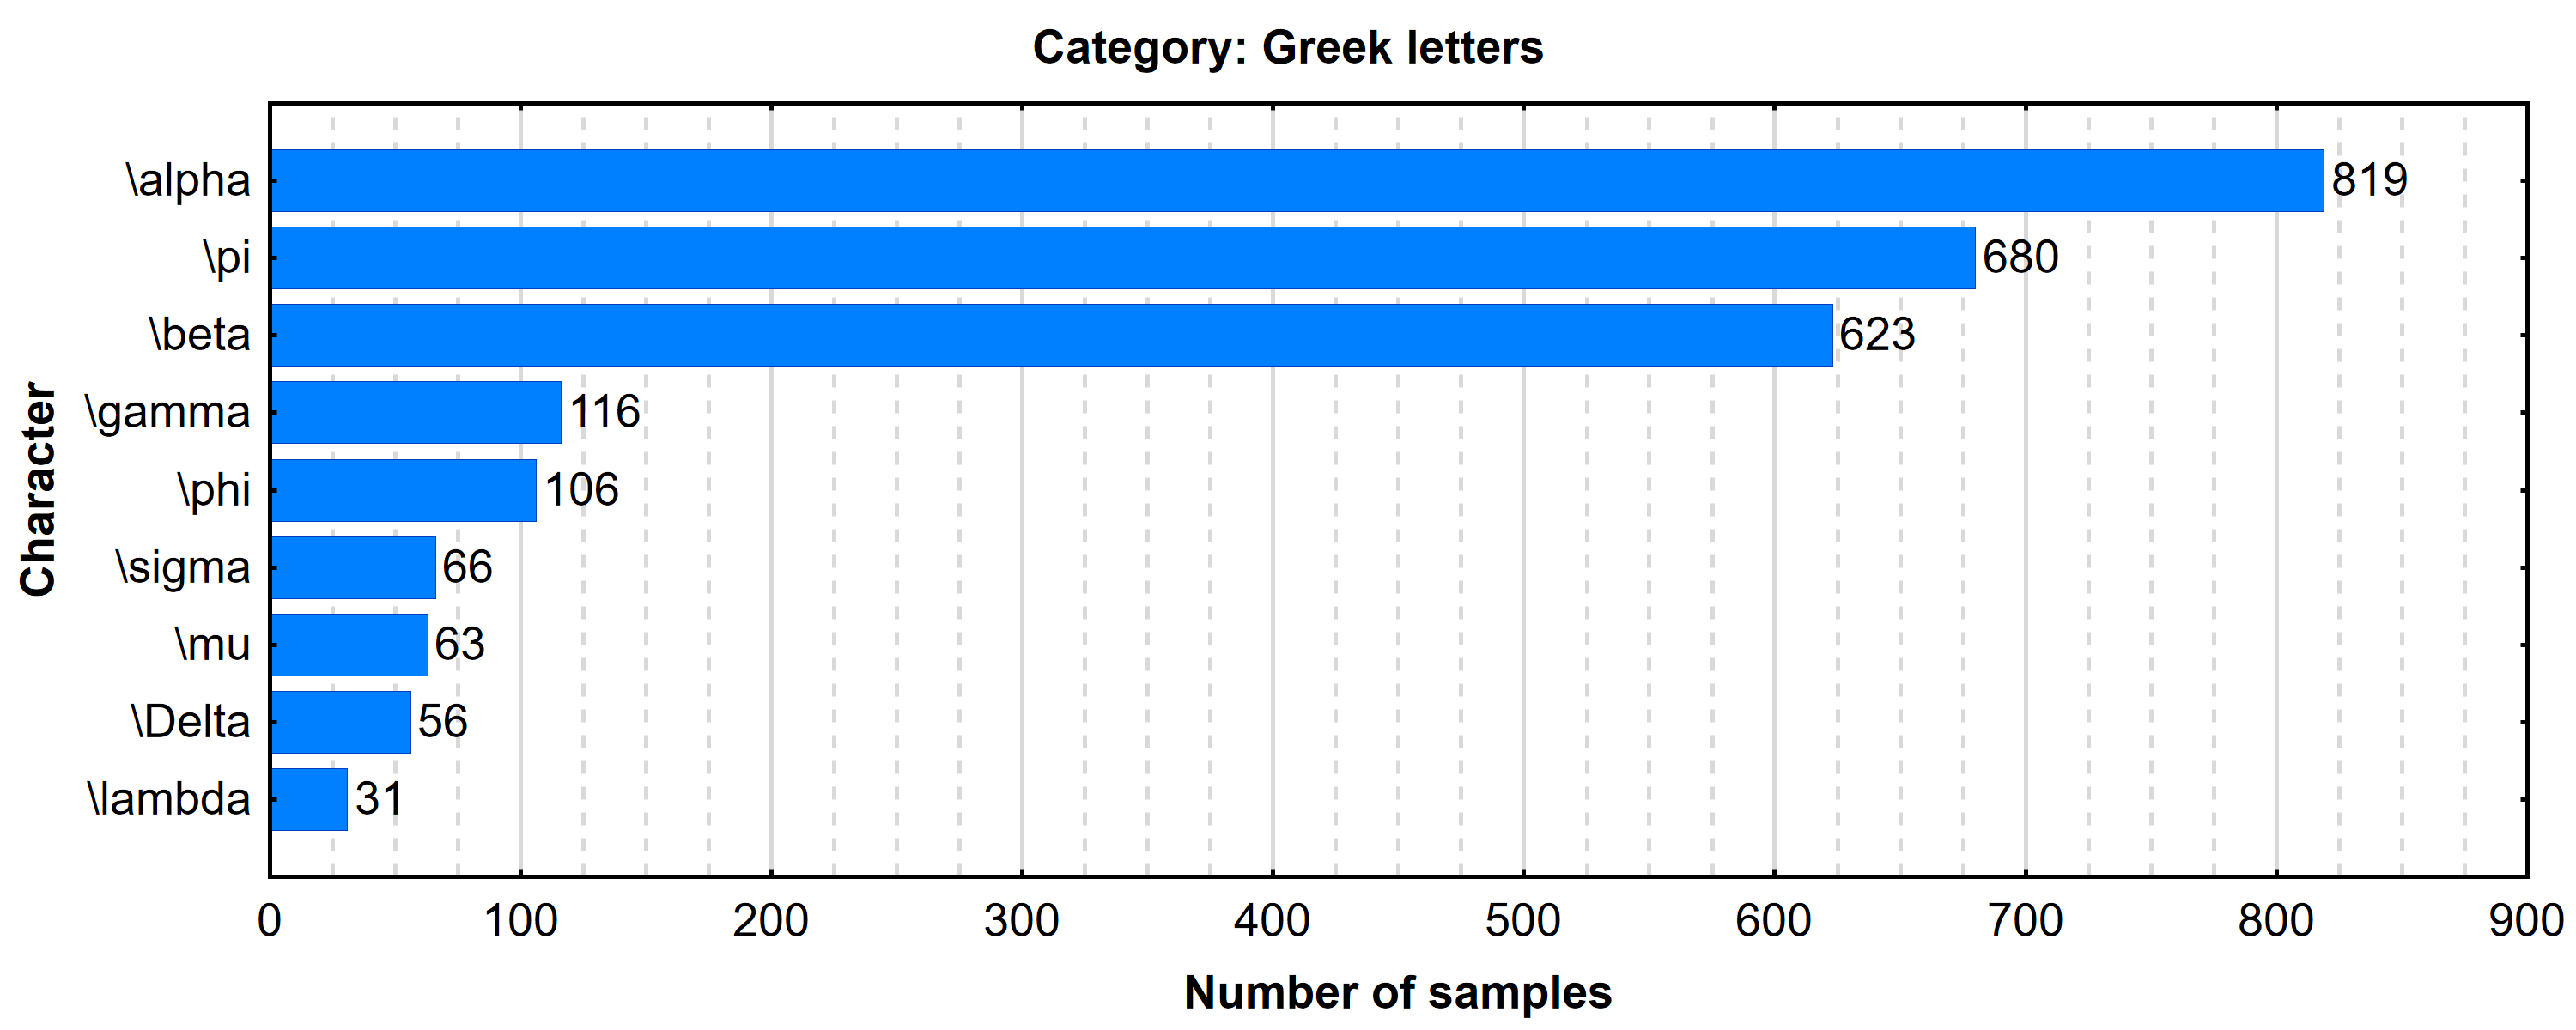
\includegraphics[width=1\textwidth]{capitulo3/imgs/greek_letters_distribution.png}
	\caption{Frecuencia de aparición de letras griegas \cite{EXTRACTOR}}
	\label{fig:GreekLetters}
\end{figure}
\newpage
Otros caracteres que aparecen en el conjunto de entrenamiento se muestran en la figura \ref{fig:SpecialSymbols} que son también de bastante utilidad como paréntesis, llaves, corchetes, el punto y la coma, que permiten definir jerarquía en las operaciones o números de punto flotante por mencionar dos aplicaciones que muestran la utilidad de los mismos. 
\begin{figure}[H]
	\centering
	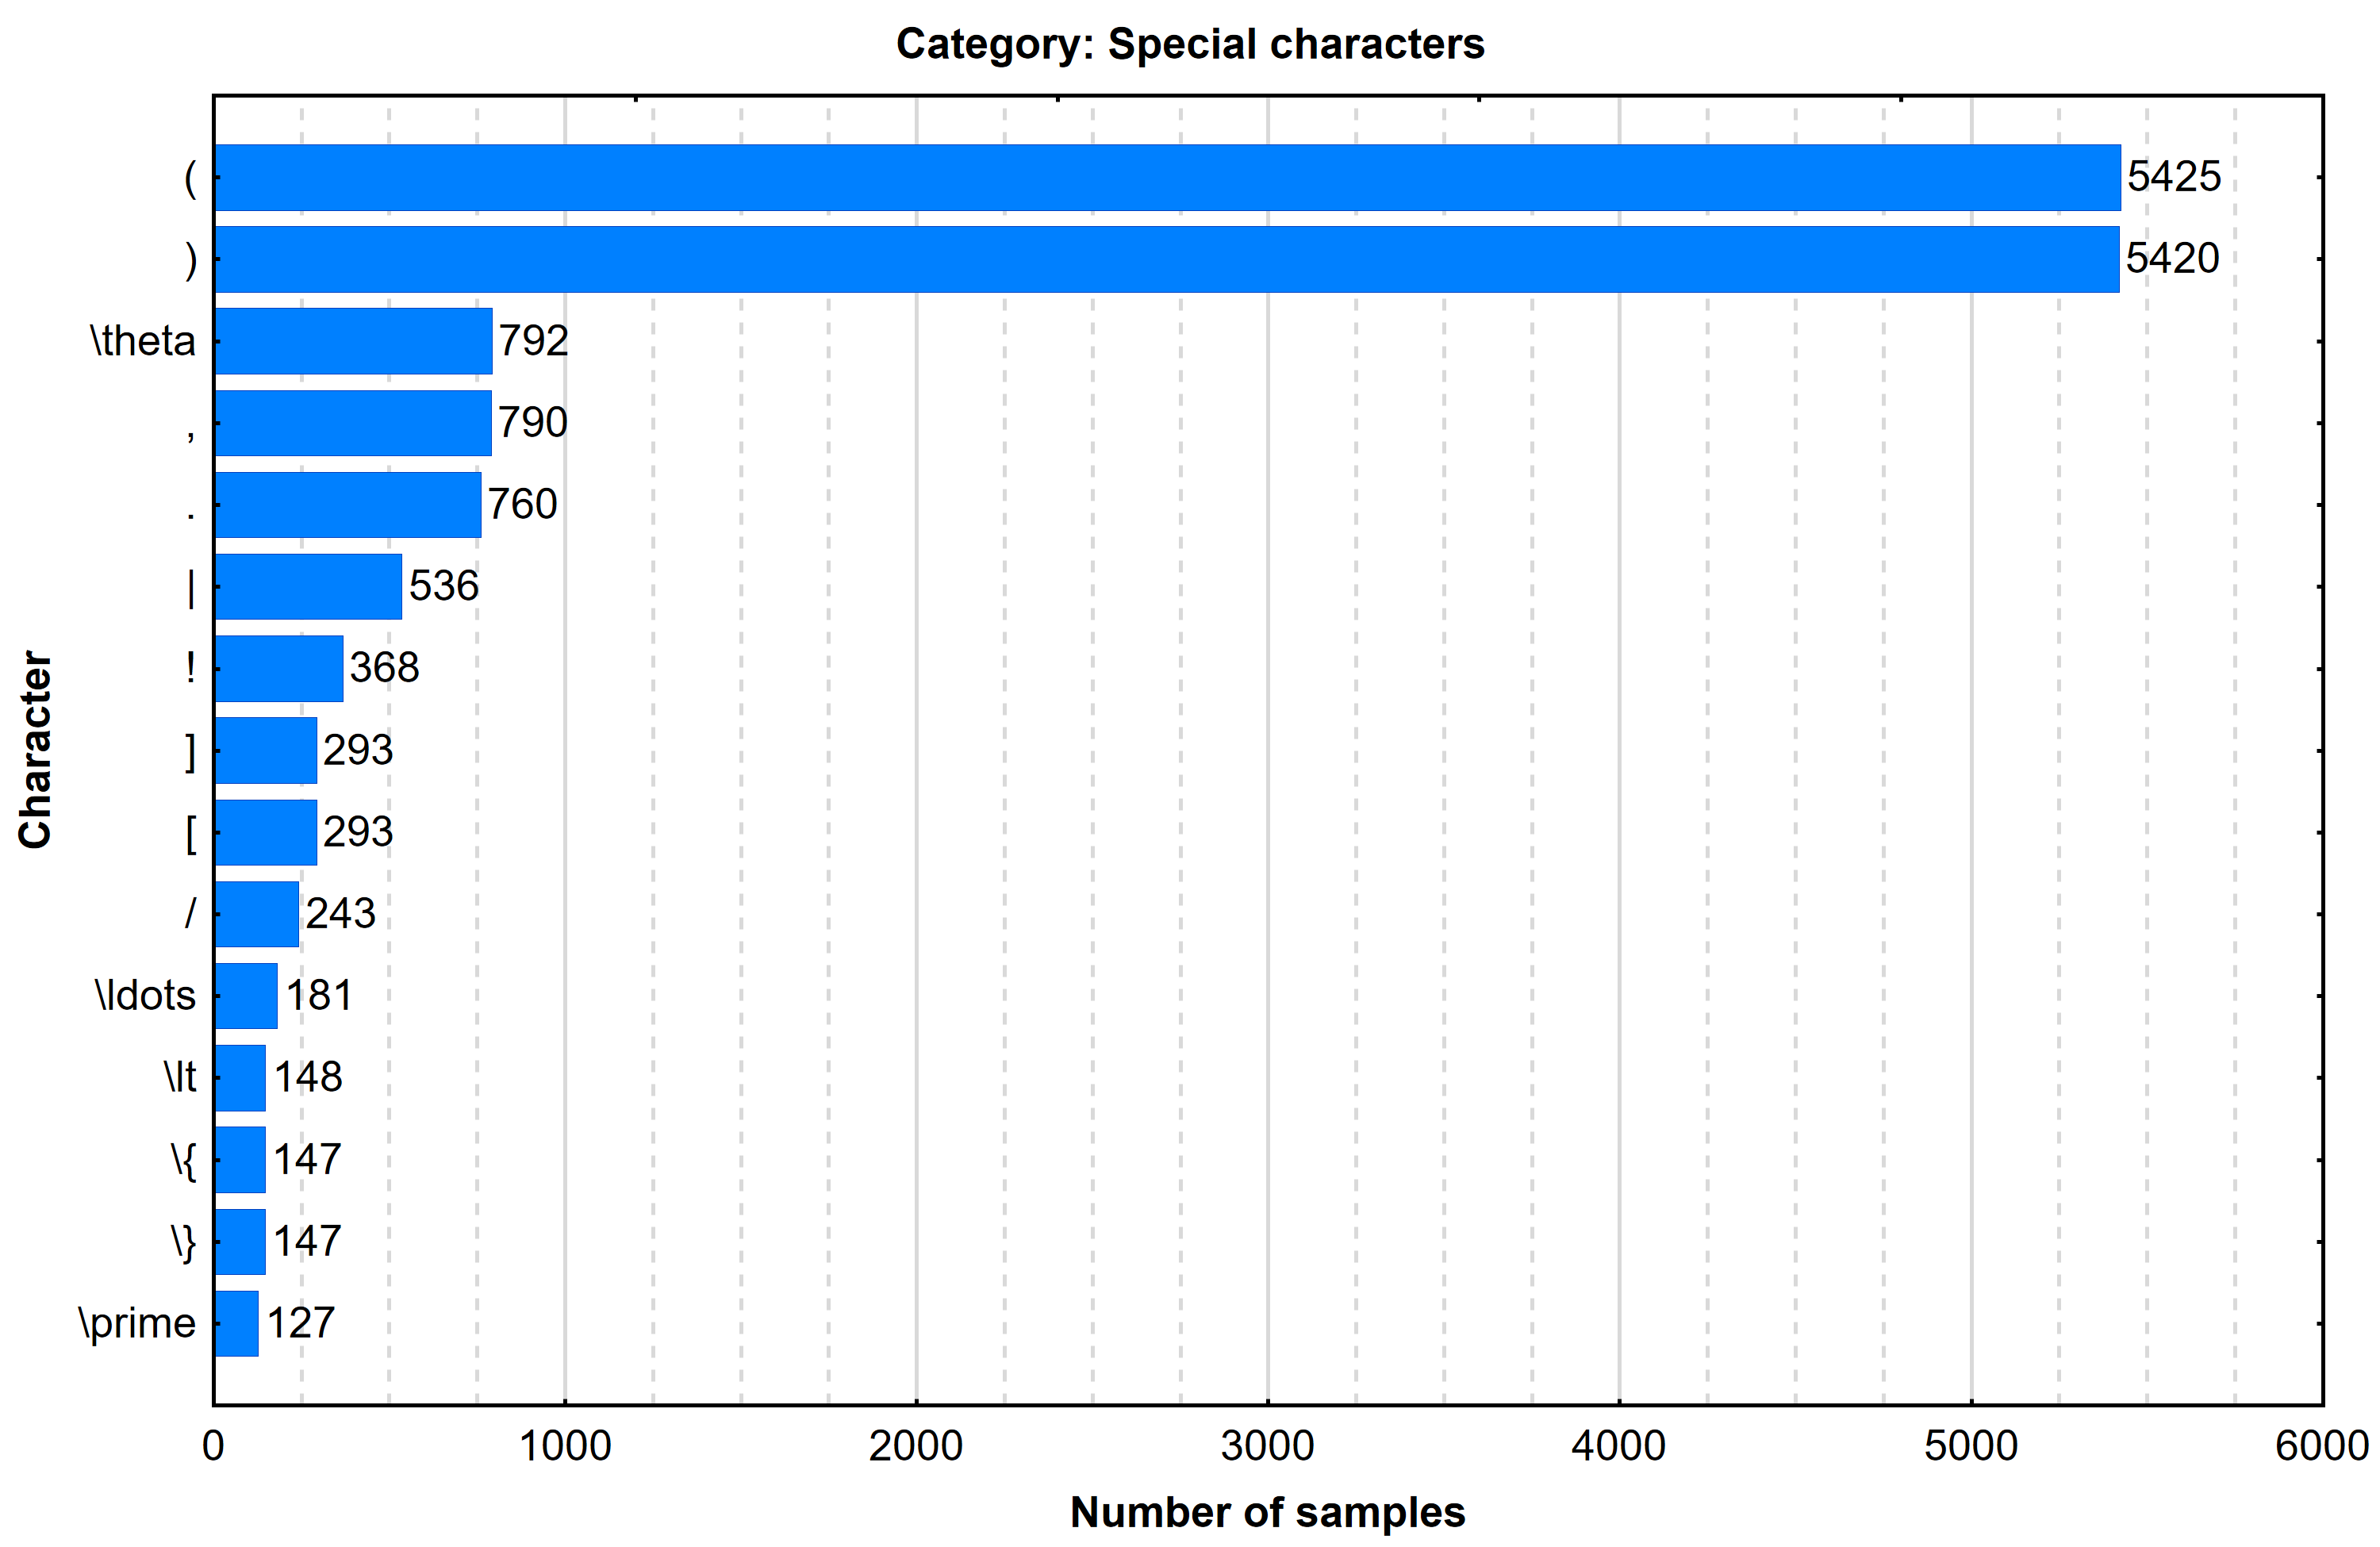
\includegraphics[width=1\textwidth]{capitulo3/imgs/special_characters_distribution.png}
	\caption{Frecuencia de aparición de símbolos especiales \cite{EXTRACTOR}}
	\label{fig:SpecialSymbols}
\end{figure}

Con estos histogramas se puede determinar qué símbolos se espera puedan ser reconocidos, así como aquellos de los cuales se esperan mejores resultados en función de su frecuencia de aparición en el conjunto de entrenamiento.

\newpage
\subsection{Nivel dimensional}
Sabiendo que el conjunto de entrenamiento CROHME no es lo suficientemente grande siendo esta una de las limitantes para obtener buenos resultados y teniendo en cuenta la bidimensionalidad que se presenta en las expresiones matemáticas, se propone el reconocimiento dos niveles en ambas direcciones, teniendo esta restricción con un mayor peso en dirección perpendicular al sentido de la escritura de las expresiones, esto basado en los resultados obtenidos por \cite{chino} 
con el mismo conjunto de entrenamiento. La figura \ref{fig:TwoDimensions} muestra un ejemplo del conjunto de entrenamiento CROHME.
%insertar Imagen
\begin{figure}[H]
	\centering
	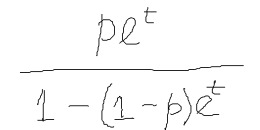
\includegraphics[width=0.6\textwidth]{capitulo3/imgs/twolevel.jpeg}
	\caption{Expresión de dos niveles vertical}
	\label{fig:TwoDimensions}
\end{figure}
\chapter{Diseño del sistema}
%Toda la documentación del sistema hay varias cosas que pueden ir aqui
%
%\begin{itemize}
%    \item Arquitectura del sistema
%    \item Diagrama de clases
%    \item Base de datos
%    \item Diagrama de paquetes
%    \item Diagrama de procesos
%    \item Casos de uso
%    \item Interfaces
%    \item Diseño de la arquitectura de la red neuronal
%\end{itemize}
%No se si tengamos que hacer todos pero al menos la arquitectura del sistema, de la red, casos de uso, interfaces y base de datos yo diría que sí



\section{Arquitectura del sistema}
\begin{figure}[h]
    \centering
    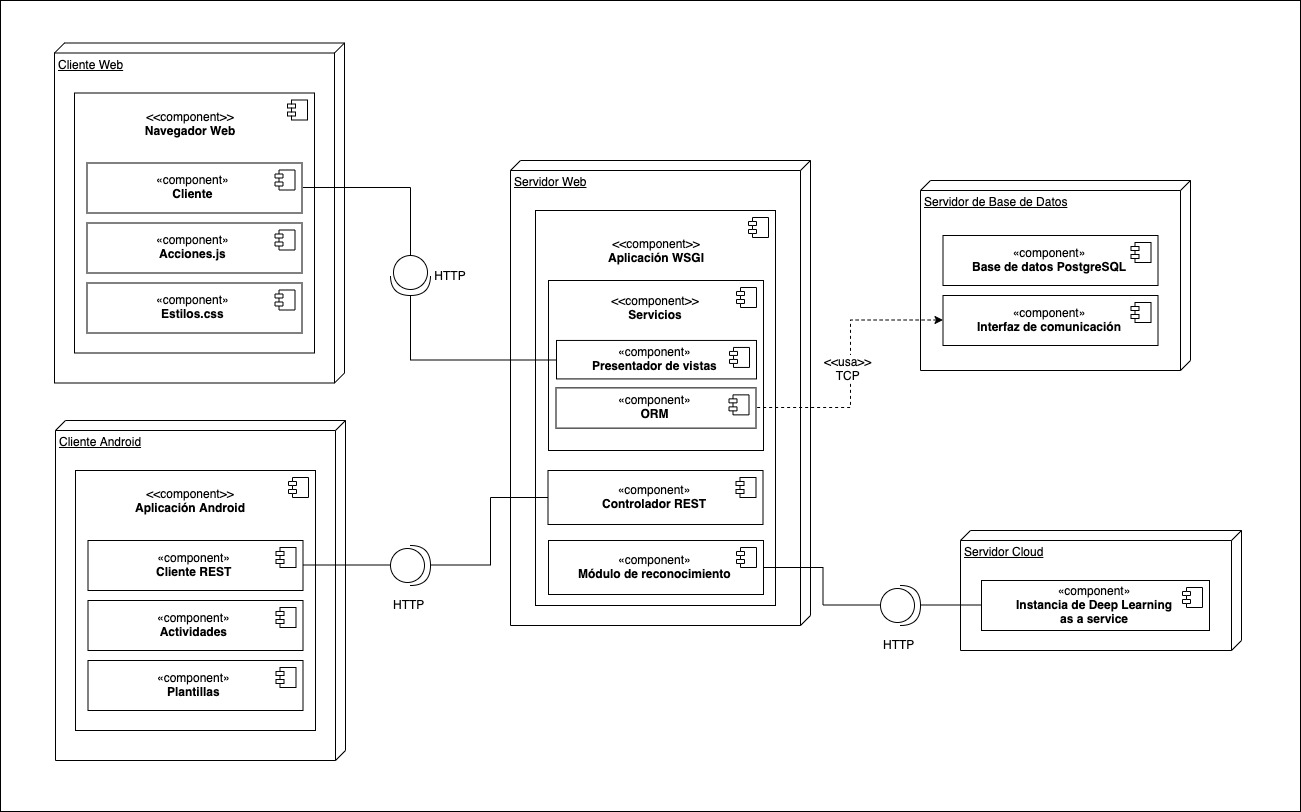
\includegraphics[width=\textwidth]{capitulo4/imagenes/ArquitecturaApp.jpg}
    \caption{Arquitectura del sistema.}
    \label{fig:arquitectura}
\end{figure}

\section{Modelo de datos del sistema}
\begin{figure}[h]
	\centering
	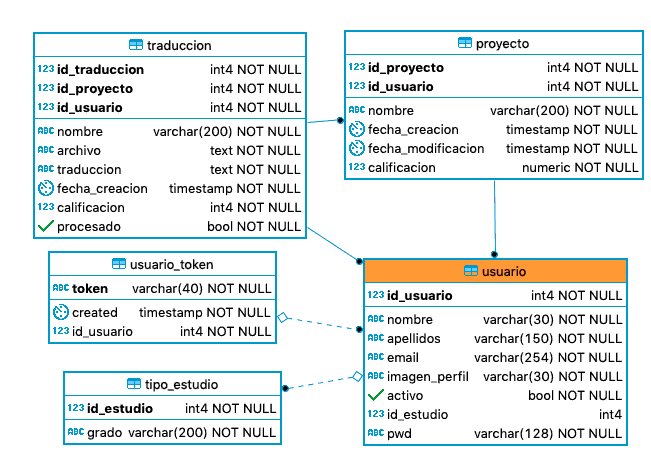
\includegraphics[width=\textwidth]{capitulo4/imagenes/tt_base.png}
	\caption{Modelo de datos del sistema.}
	\label{fig:db}
\end{figure}

\subsection{Entidad: Usuario}
Se refiere a la cuenta que un usuario puede tener, es la forma en la que accede al sistema.
\subsubsection{Atributos}
\begin{center}
	\begin{longtable}{|J{4cm}|J{4cm}|J{3cm}|J{2cm}|J{2cm}|}
		\hline
		\textbf{Nombre} & \textbf{Descripción} & \textbf{Tipo} & \textbf{Requerido} & \textbf{Único} \\ \hline
		\caption{Tabla de los atributos de la entidad usuario}
		\label{tbl:entidad-usuario}
	\end{longtable}
\end{center}
\subsection{Entidad: Proyecto}
Se refiere a los proyectos que están asociados a un usuario, un proyecto esta compuesto por varias traducciones.
\subsubsection{Atributos}
\begin{center}
	\begin{longtable}{|J{4cm}|J{4cm}|J{3cm}|J{2cm}|J{2cm}|}
		\hline
		\textbf{Nombre} & \textbf{Descripción} & \textbf{Tipo} & \textbf{Requerido} & \textbf{Único} \\ \hline
		\caption{Tabla de los atributos de la entidad proyecto}
		\label{tbl:entidad-proyecto}
	\end{longtable}
\end{center}
\subsection{Entidad: Traducción}
Hace referencia a la traducción de \LaTeX que forma parte de un proyecto y que pertenece a un usuario. Esta traducción es el resultado de analizar una imagen.
\subsubsection{Atributos}
\begin{center}
	\begin{longtable}{|J{4cm}|J{4cm}|J{3cm}|J{2cm}|J{2cm}|}
		\hline
		\textbf{Nombre} & \textbf{Descripción} & \textbf{Tipo} & \textbf{Requerido} & \textbf{Único} \\ \hline
		\caption{Tabla de los atributos de la entidad traducción}
		\label{tbl:entidad-traduccion}
	\end{longtable}
\end{center}
\subsection{Entidad: Tipo estudios}
Hace referencia a los distintos grados de estudios que tiene un usuario.
\subsubsection{Atributos}
\begin{center}
	\begin{longtable}{|J{4cm}|J{4cm}|J{3cm}|J{2cm}|J{2cm}|}
		\hline
		\textbf{Nombre} & \textbf{Descripción} & \textbf{Tipo} & \textbf{Requerido} & \textbf{Único} \\ \hline
		\caption{Tabla de los atributos de la entidad tipo de estudios}
		\label{tbl:entidad-tipo-estudios}
	\end{longtable}
\end{center}
\subsection{Entidad: Usuario Token}
Se refiere al token de autenticación que tiene un usuario al momento de crear una cuenta y que su utiliza en la comunicación entre la aplicación web y android.
\subsubsection{Atributos}
\begin{center}
	\begin{longtable}{|J{4cm}|J{4cm}|J{3cm}|J{2cm}|J{2cm}|}
		\hline
		\textbf{Nombre} & \textbf{Descripción} & \textbf{Tipo} & \textbf{Requerido} & \textbf{Único} \\ \hline
		\caption{Tabla de los atributos de la entidad usuario token}
		\label{tbl:entidad-usuario-token}
	\end{longtable}
\end{center}

\section{Aplicación de Android}
\section{Android}
Esta sección tiene objetivo presentar las principales características en el desarrollo de la aplicación para Android.
\subsection{Arquitectura de la aplicación}
Para el desarrollo de la aplicación se implemento la arquitectura Clean, la cual como ya se ha mencionado antes se ha mencionado se ha vuelto muy popular en el desarrollo de aplicaciones móviles para android debido a que es una solución que produce sistemas que presentan las siguientes características.

\begin{itemize}
    \item Escalables, por lo que se pueden agregar más funcionalidades de forma sencilla.
    \item Presentan modularidad.
    \item Presentan independencia en cuanto a frameworks, interfaz de usuario y bases de datos.
    \item El proyecto es más fácil de mantener por lo que es más sencillo hacer cambios.
\end{itemize}

Al utilizar esta arquitectura el proyecto queda separado en tres capas como se observa en la figura \ref{fig:capas-arquitectura} con lo cual cada una de ellas tiene su propósito definido.

\begin{figure}[h]
    \centering
    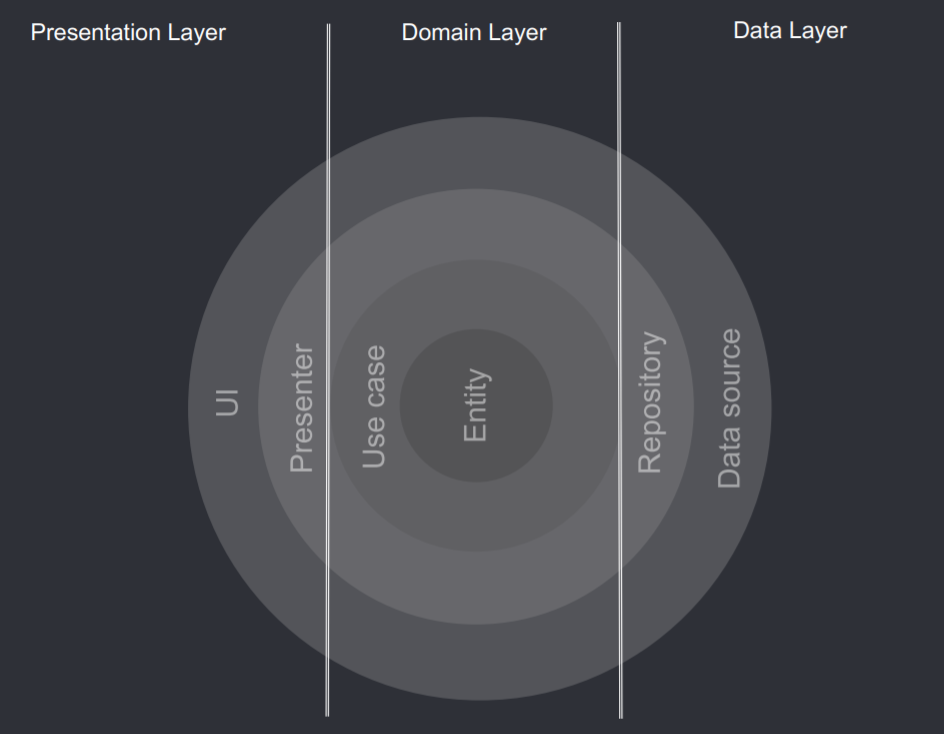
\includegraphics[width=250px]{capitulo5/android/img/capas-clean.png}
    \caption{Tres capas que se tienen al utilizar la arquitectura Clean \cite{cleanGuide}}
    \label{fig:capas-arquitectura}
\end{figure}

\subsubsection{Capa de datos}
La información que se utiliza en el resto de capas proviene de esta capa. Esta capa a su vez se encuentra dividida en la capa de repositorio y en la capa de fuente de datos. 

\paragraph{Capa de repositorio} En esta capa se utiliza el patrón de repositorio como se muestra en la figura \ref{fig:capa-datos}. Gracias a este patrón se puede tener acceso a diferentes fuentes de datos que se encuentran en la capa más baja de nuestra arquitectura, esto nos permite un acceso a los datos de forma transparente para el usuario bajo las condiciones que se presenten.

La forma de utilizar este patrón en la aplicación desarrollado crear una clase en la cual se hace uso de la interfaz que se tiene para el acceso a la fuente de datos. En el siguiente código se puede apreciar el como se crea una instancia de APIService que es nuestra interfaz para fuente de datos.

Después, en nuestro método findAllProyecttosByUser se recupera la información necesaria para mandarla a las capas superiores.

\lstinputlisting[language=Java]{capitulo5/android/src/repositorio.java}

\begin{figure}[h]
    \centering
    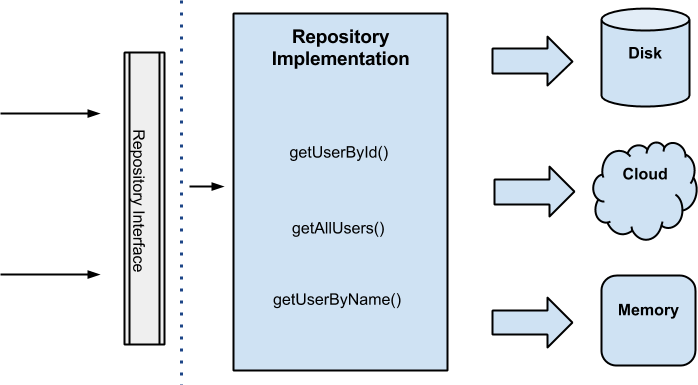
\includegraphics[width=400px]{capitulo5/android/img/capa-datos.png}
    \caption{Capa de datos \cite{cleanWay}}
    \label{fig:capa-datos}
\end{figure}

\paragraph{Capa de fuente de datos} En este trabajo, la fuente de datos que se tiene es un API REST, sin embargo si se requiere acceder a información que se persista en el teléfono se pude agregar otra fuente de datos. Se utilizó retrofit para poder realizar la comunicación con el API REST. 

La forma de utilizar retrofit es crear una interfaz con todos los métodos para recuperar o enviar información al API REST, en esta interfaz cada método tiene la URL a la cual se realizara la petición con alguno de los métodos que tiene HTTP, se tienen los parámetro que se envían y cada método nos regresa una llamada asíncrona que se trabaja en la capa de repositorio. Esto se puede apreciar en el siguiente código.

\lstinputlisting[language=Java]{capitulo5/android/src/APIService.java}

Para poder hacer uso de esta interfaz se tiene que configurar bajo ciertas características especificas como lo son la URL a la cual hará peticiones, el logger que se utilizara para poder observar las peticiones que se realizan y brindar una retroalimentación a la hora de hacer pruebas y por ultimo el parser que se utilizara para trabajar y pasar de clases a datos que el API REST entienda y pueda utilizar, en este caso se utilizo el formato JSON. La definición de estas características se tiene en el siguiente código.

\lstinputlisting[language=Java]{capitulo5/android/src/ServiceGenerator.java}

Finalmente, en esta capa se tienen clases Java que después se mapean a objetos JSON y viceversa, para realizar esto se crea un POJO con los atributos que se necesitan además de agregar anotaciones de retrofit para que el parser pude hacer la conversión necesaria. Un ejemplo de esto es en la siguiente clase de java.

\lstinputlisting[language=Java]{capitulo5/android/src/UsuarioData.java}


\subsubsection{Capa de dominio}
En esta capa es la intermediaria entre las otras dos capas que se tienen, es donde se encuentran los casos de uso también conocidos como interactors como se muestra en la figura \ref{fig:capa-dominio} en ellos la lógica del negocio es ejecutada es por esto que es el núcleo de la aplicación.

Es importante mencionar que esta capa, al ser la encargada del negocio es donde se hacen validaciones en la información y dicha información se adapta para que sea trabajada en la capa de presentación o en la de datos

Además de contener los casos de uso en esta capa se encuentran las entidades y se hace uso de los repositorios para acceder a la información proporcionada por la capa de datos.

\begin{figure}[h]
    \centering
    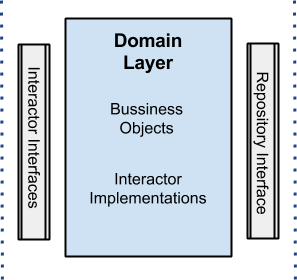
\includegraphics[width=200px]{capitulo5/android/img/capa-dominio.png}
    \caption{Capa de dominio \cite{cleanWay}}
    \label{fig:capa-dominio}
\end{figure}

Para tener un control sobre posibles errores en la capa de presentación o en la capa de datos se utilizan códigos de resultados al igual que una clase que contiene el resultado que se puede presentar, así como la información que se le regresa a la capa de presentación. Se hace uso de genéricos para poder reutilizar esta clase en toda la aplicación y no duplicar código. La clase es la siguiente.

\lstinputlisting[language=Java]{capitulo5/android/src/BusinessResult.java}

La forma en la que se utiliza esta clase en un caso de uso se presenta en el siguiente código que permite iniciar sesión.

\lstinputlisting[language=Java]{capitulo5/android/src/UserInteractorImpl.java}

A su vez el caso de uso utiliza sus propios clases de java para presentar información al usuario en la capa de presentación así como controlar posibles errores en la información que ingrese el usuario los campos de los formularios, un ejemplo de este tipo de clases es el siguiente.

\lstinputlisting[language=Java]{capitulo5/android/src/UsuarioModel.java}

\subsubsection{Capa de presentación}
En esta capa como se muestra en la figura \ref{fig:capa-presentacion} se trabaja con la lógica relacionada a las interfaces que se tienen en la aplicación, es decir a actividades, fragmentos y archivos XML.

\begin{figure}[h]
    \centering
    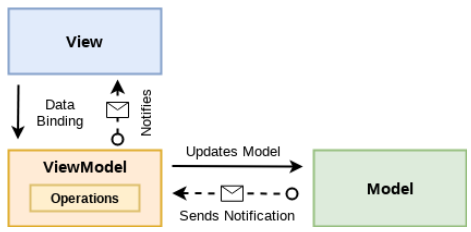
\includegraphics[width=300px]{capitulo5/android/img/capa-presentacion.png}
    \caption{Capa de presentación \cite{cleanWayReload}}
    \label{fig:capa-presentacion}
\end{figure}

En esta capa se pueden trabajar con patrones como MVC y MVP pero en este caso se utiliza el patrón MVVM cada uno con una función en particular. \cite{cleanWayReload}

\begin{itemize}
    \item \textbf{Modelo} Se encarga de representar la información que sera presentada en la vista.
    \item \textbf{Vista} Compuesta en este caso por las actividades y fragmentos de la aplicación, su tarea es mostrar la información, hacen uso de los viewmodels para poder realizar cambios en la interfaz.
    \item \textbf{ViewModel} El ViewModel sera el encargado de ejecutar los casos de uso o interactors con el objetivo de actualizar la vista de acuerdo a la información que presente el modelo.
\end{itemize}



\newpage
\section{Aplicación Web}
\section{Android}
Esta sección tiene objetivo presentar las principales características en el desarrollo de la aplicación para Android.
\subsection{Arquitectura de la aplicación}
Para el desarrollo de la aplicación se implemento la arquitectura Clean, la cual como ya se ha mencionado antes se ha mencionado se ha vuelto muy popular en el desarrollo de aplicaciones móviles para android debido a que es una solución que produce sistemas que presentan las siguientes características.

\begin{itemize}
    \item Escalables, por lo que se pueden agregar más funcionalidades de forma sencilla.
    \item Presentan modularidad.
    \item Presentan independencia en cuanto a frameworks, interfaz de usuario y bases de datos.
    \item El proyecto es más fácil de mantener por lo que es más sencillo hacer cambios.
\end{itemize}

Al utilizar esta arquitectura el proyecto queda separado en tres capas como se observa en la figura \ref{fig:capas-arquitectura} con lo cual cada una de ellas tiene su propósito definido.

\begin{figure}[h]
    \centering
    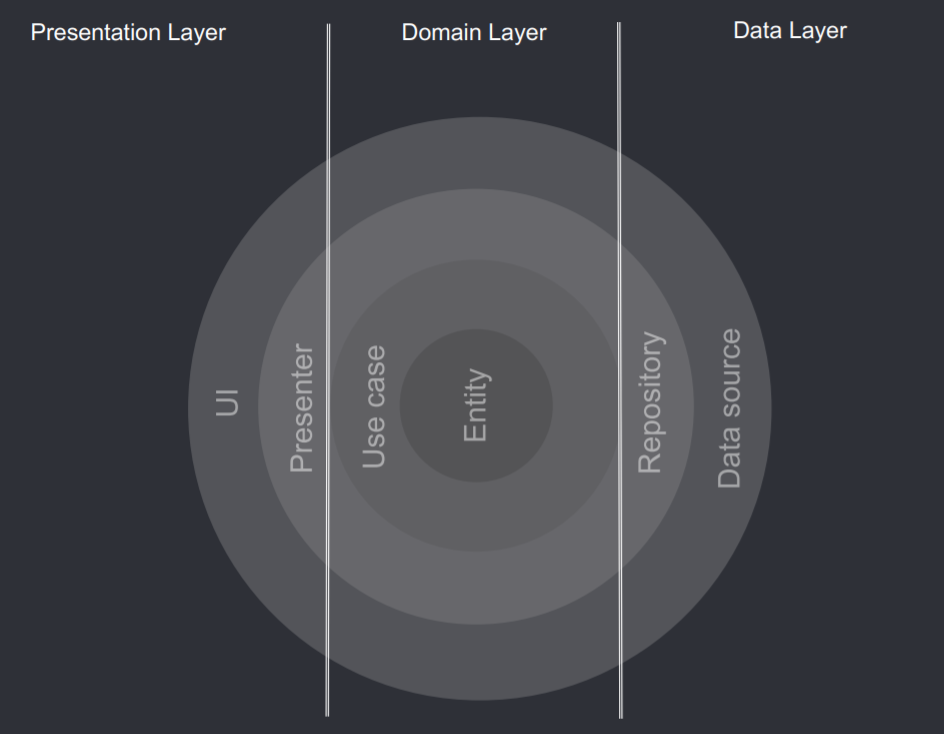
\includegraphics[width=250px]{capitulo5/android/img/capas-clean.png}
    \caption{Tres capas que se tienen al utilizar la arquitectura Clean \cite{cleanGuide}}
    \label{fig:capas-arquitectura}
\end{figure}

\subsubsection{Capa de datos}
La información que se utiliza en el resto de capas proviene de esta capa. Esta capa a su vez se encuentra dividida en la capa de repositorio y en la capa de fuente de datos. 

\paragraph{Capa de repositorio} En esta capa se utiliza el patrón de repositorio como se muestra en la figura \ref{fig:capa-datos}. Gracias a este patrón se puede tener acceso a diferentes fuentes de datos que se encuentran en la capa más baja de nuestra arquitectura, esto nos permite un acceso a los datos de forma transparente para el usuario bajo las condiciones que se presenten.

La forma de utilizar este patrón en la aplicación desarrollado crear una clase en la cual se hace uso de la interfaz que se tiene para el acceso a la fuente de datos. En el siguiente código se puede apreciar el como se crea una instancia de APIService que es nuestra interfaz para fuente de datos.

Después, en nuestro método findAllProyecttosByUser se recupera la información necesaria para mandarla a las capas superiores.

\lstinputlisting[language=Java]{capitulo5/android/src/repositorio.java}

\begin{figure}[h]
    \centering
    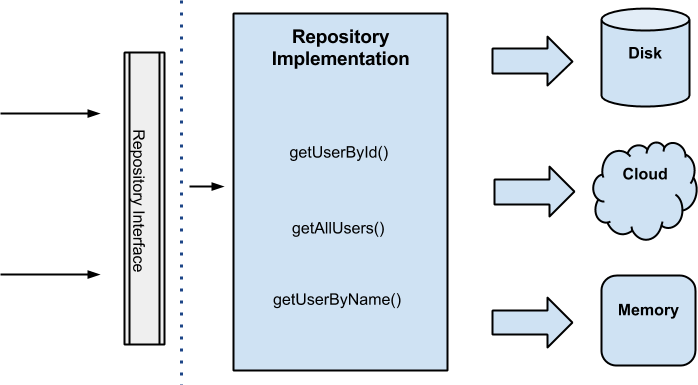
\includegraphics[width=400px]{capitulo5/android/img/capa-datos.png}
    \caption{Capa de datos \cite{cleanWay}}
    \label{fig:capa-datos}
\end{figure}

\paragraph{Capa de fuente de datos} En este trabajo, la fuente de datos que se tiene es un API REST, sin embargo si se requiere acceder a información que se persista en el teléfono se pude agregar otra fuente de datos. Se utilizó retrofit para poder realizar la comunicación con el API REST. 

La forma de utilizar retrofit es crear una interfaz con todos los métodos para recuperar o enviar información al API REST, en esta interfaz cada método tiene la URL a la cual se realizara la petición con alguno de los métodos que tiene HTTP, se tienen los parámetro que se envían y cada método nos regresa una llamada asíncrona que se trabaja en la capa de repositorio. Esto se puede apreciar en el siguiente código.

\lstinputlisting[language=Java]{capitulo5/android/src/APIService.java}

Para poder hacer uso de esta interfaz se tiene que configurar bajo ciertas características especificas como lo son la URL a la cual hará peticiones, el logger que se utilizara para poder observar las peticiones que se realizan y brindar una retroalimentación a la hora de hacer pruebas y por ultimo el parser que se utilizara para trabajar y pasar de clases a datos que el API REST entienda y pueda utilizar, en este caso se utilizo el formato JSON. La definición de estas características se tiene en el siguiente código.

\lstinputlisting[language=Java]{capitulo5/android/src/ServiceGenerator.java}

Finalmente, en esta capa se tienen clases Java que después se mapean a objetos JSON y viceversa, para realizar esto se crea un POJO con los atributos que se necesitan además de agregar anotaciones de retrofit para que el parser pude hacer la conversión necesaria. Un ejemplo de esto es en la siguiente clase de java.

\lstinputlisting[language=Java]{capitulo5/android/src/UsuarioData.java}


\subsubsection{Capa de dominio}
En esta capa es la intermediaria entre las otras dos capas que se tienen, es donde se encuentran los casos de uso también conocidos como interactors como se muestra en la figura \ref{fig:capa-dominio} en ellos la lógica del negocio es ejecutada es por esto que es el núcleo de la aplicación.

Es importante mencionar que esta capa, al ser la encargada del negocio es donde se hacen validaciones en la información y dicha información se adapta para que sea trabajada en la capa de presentación o en la de datos

Además de contener los casos de uso en esta capa se encuentran las entidades y se hace uso de los repositorios para acceder a la información proporcionada por la capa de datos.

\begin{figure}[h]
    \centering
    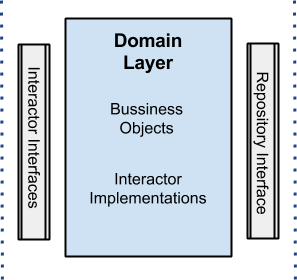
\includegraphics[width=200px]{capitulo5/android/img/capa-dominio.png}
    \caption{Capa de dominio \cite{cleanWay}}
    \label{fig:capa-dominio}
\end{figure}

Para tener un control sobre posibles errores en la capa de presentación o en la capa de datos se utilizan códigos de resultados al igual que una clase que contiene el resultado que se puede presentar, así como la información que se le regresa a la capa de presentación. Se hace uso de genéricos para poder reutilizar esta clase en toda la aplicación y no duplicar código. La clase es la siguiente.

\lstinputlisting[language=Java]{capitulo5/android/src/BusinessResult.java}

La forma en la que se utiliza esta clase en un caso de uso se presenta en el siguiente código que permite iniciar sesión.

\lstinputlisting[language=Java]{capitulo5/android/src/UserInteractorImpl.java}

A su vez el caso de uso utiliza sus propios clases de java para presentar información al usuario en la capa de presentación así como controlar posibles errores en la información que ingrese el usuario los campos de los formularios, un ejemplo de este tipo de clases es el siguiente.

\lstinputlisting[language=Java]{capitulo5/android/src/UsuarioModel.java}

\subsubsection{Capa de presentación}
En esta capa como se muestra en la figura \ref{fig:capa-presentacion} se trabaja con la lógica relacionada a las interfaces que se tienen en la aplicación, es decir a actividades, fragmentos y archivos XML.

\begin{figure}[h]
    \centering
    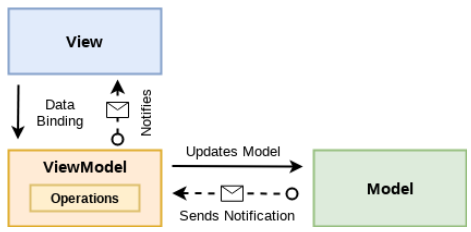
\includegraphics[width=300px]{capitulo5/android/img/capa-presentacion.png}
    \caption{Capa de presentación \cite{cleanWayReload}}
    \label{fig:capa-presentacion}
\end{figure}

En esta capa se pueden trabajar con patrones como MVC y MVP pero en este caso se utiliza el patrón MVVM cada uno con una función en particular. \cite{cleanWayReload}

\begin{itemize}
    \item \textbf{Modelo} Se encarga de representar la información que sera presentada en la vista.
    \item \textbf{Vista} Compuesta en este caso por las actividades y fragmentos de la aplicación, su tarea es mostrar la información, hacen uso de los viewmodels para poder realizar cambios en la interfaz.
    \item \textbf{ViewModel} El ViewModel sera el encargado de ejecutar los casos de uso o interactors con el objetivo de actualizar la vista de acuerdo a la información que presente el modelo.
\end{itemize}



\newpage
\section{Mensajes}
En esta sección se muestran los mensajes que se despliegan en pantalla para los diferentes casos de uso que se tienen.
\begin{enumerate}[label=MSG\arabic*.]
    \item \label{MSG1}
        \begin{description}
            \item \textbf{MSG1 Datos no validos}
            \item [Tipo] Error
            \item [Redacción] Los datos introducidos no son validos.
            %\item [Parametros]
             %\item [Ejemplo]
        \end{description}
    \item \label{MSG2}
        \begin{description}
            \item \textbf{MSG2 Cuenta no verificada}
            \item [Tipo] Error
            \item [Redacción] La cuenta aun no ha sido verificada.
        \end{description}
    \item \label{MSG3}
        \begin{description}
            \item \textbf{MSG3 Correo electrónico no registrado}
            \item [Tipo] Error
            \item [Redacción] No existe una cuenta con el correo electrónico introducido.
        \end{description}
    \item \label{MSG4}
        \begin{description}
            \item \textbf{MSG4 Correo electrónico ya registrado}
            \item [Tipo] Error
            \item [Redacción] El correo electrónico ya se ha utilizado.
        \end{description}
    \item \label{MSG5}
        \begin{description}
            \item \textbf{MSG5 Verifique su cuenta}
            \item [Tipo] Informativo
            \item [Redacción] Verifique su cuenta a través del correo electrónico que se le ha mandado.
        \end{description}
    \item \label{MSG6}
        \begin{description}
            \item \textbf{MSG6 Envio de correo de recuperación}
            \item [Tipo] Informativo
            \item [Redacción] Se ha enviado un correo electrónico para la recuperación de su contraseña.
        \end{description}
    \item \label{MSG7}
        \begin{description}
            \item \textbf{MSG7 No existen proyectos para mostrar}
            \item [Tipo] Informativo
            \item [Redacción] No hay proyectos que se puedan mostrar.
        \end{description}
    \item \label{MSG8}
        \begin{description}
            \item \textbf{MSG8 No se puede mostrar el proyecto}
            \item [Tipo] Error
            \item [Redacción] En este momento no se puede mostrar el proyecto.
        \end{description}
    \item \label{MSG9}
        \begin{description}
            \item \textbf{MSG9 Operación exitosa}
            \item [Tipo] Informativo
            \item [Redacción] La operación se ha realizado con éxito.
        \end{description}
    \item \label{MSG10}
        \begin{description}
            \item \textbf{MSG10 Operación fallida}
            \item [Tipo] Error
            \item [Redacción] La operación no se pudo realizar.
        \end{description}
    \item \label{MSG11}
        \begin{description}
            \item \textbf{MSG11 Confirmación de operación}
            \item [Tipo] Confirmación
            \item [Redacción] \hfill \\
            ¿Está seguro de $<$OPERACIÓN$>$ $<$ELEMENTO$>$ $<$NOMBRE\textunderscore ELEMENTO$>$?
            \item [Parametros] \hfill
                \begin{itemize} 
                    \item $<$OPERACIÓN$>$: Operación a realizar que se debe de confirmar.
                    \item $<$ELEMENTO$>$: Elemento sobre el cual se realizara la operación.
                    \item $<$NOMBRE\textunderscore ELEMENTO$>$: Nombre del elemento sobre el que se trabaja.
                \end{itemize}
            \item [Ejemplo] \hfill
                \begin{itemize}
                    \item ¿Está seguro de eliminar el proyecto tesis final?
                \end{itemize}
        \end{description}
    \item \label{MSG12}
        \begin{description}
            \item \textbf{MSG12 Ingrese el nombre}
            \item [Tipo] Confirmación
            \item [Redacción] Ingrese el nombre del proyecto.
        \end{description}
    \item \label{MSG13}
        \begin{description}
            \item \textbf{MSG13 Falta información}
            \item [Tipo] Error
            \item [Redacción] Falta información necesaria para realizar la operación.
        \end{description}
\end{enumerate}

\newpage
\section{Interfaces}
\subsection{Aplicación en Android}
\begin{figure}[h]
    \centering
    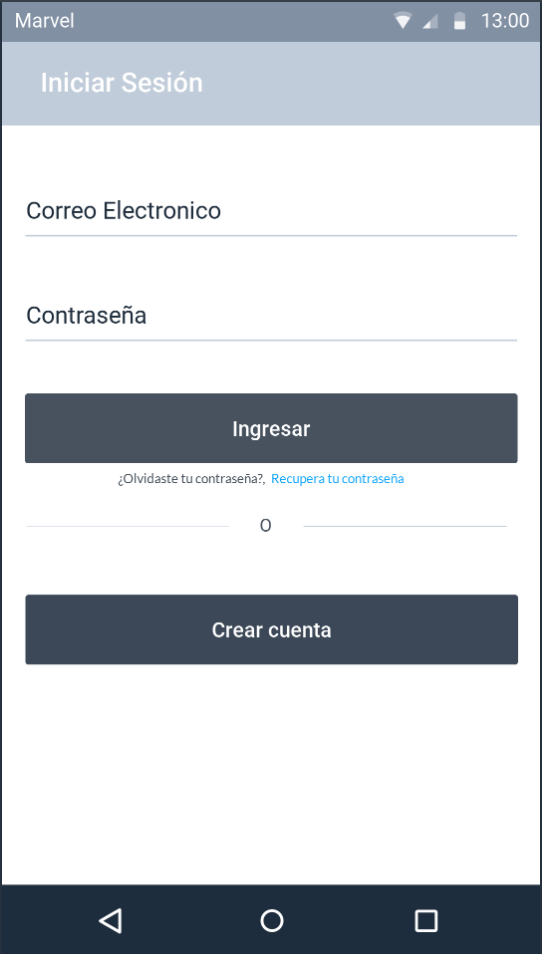
\includegraphics[width=200px]{capitulo4/imagenes/android/MIUA_1.png}
    \caption{MIUA 1 Iniciar Sesión}
    \label{fig:MIUA-1} %MOCK UP DE INTERFAZ DE USUARIO ANDROID
\end{figure}

\begin{figure}[h]
    \centering
    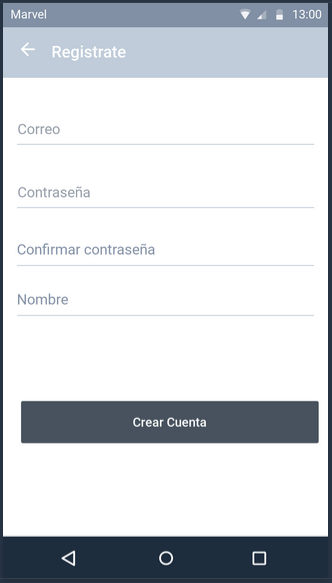
\includegraphics[width=200px]{capitulo4/imagenes/android/MIUA_2.png}
    \caption{MIUA 2 Registro}
    \label{fig:MIUA-2} %MOCK UP DE INTERFAZ DE USUARIO ANDROID
\end{figure}

\begin{figure}[h]
    \centering
    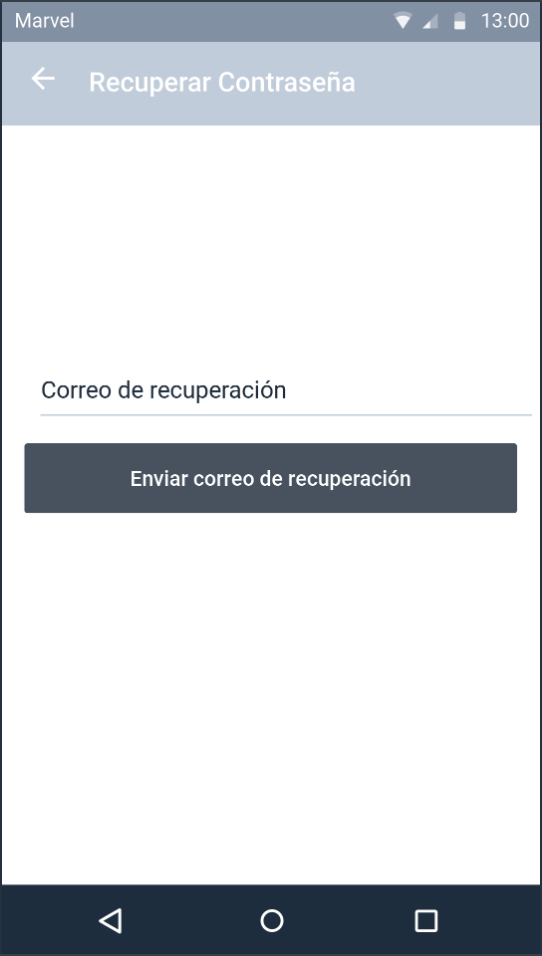
\includegraphics[width=200px]{capitulo4/imagenes/android/MIUA_3.png}
    \caption{MIUA 3 Recuperar Contraseña}
    \label{fig:MIUA-3} %MOCK UP DE INTERFAZ DE USUARIO ANDROID
\end{figure}

\begin{figure}[h]
    \centering
    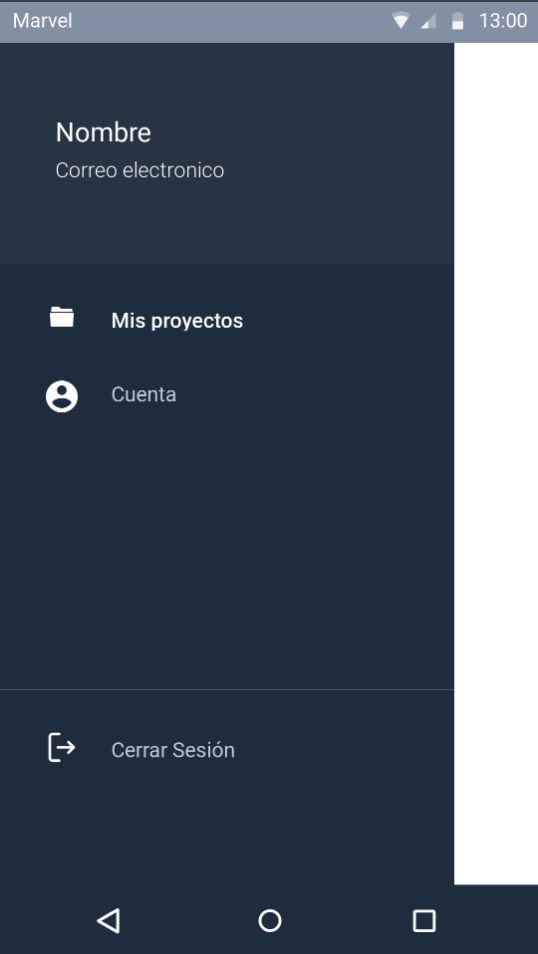
\includegraphics[width=200px]{capitulo4/imagenes/android/MIUA_4.png}
    \caption{MIUA 4 Menú de Opciones}
    \label{fig:MIUA-4} %MOCK UP DE INTERFAZ DE USUARIO ANDROID
\end{figure}

\begin{figure}[h]
    \centering
    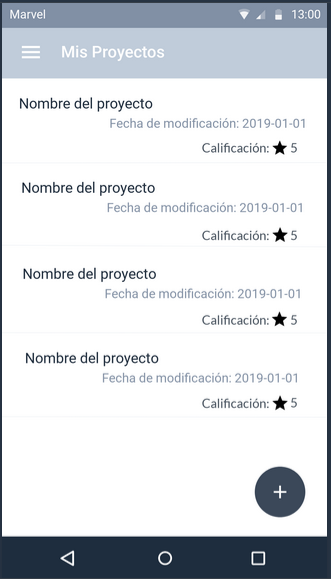
\includegraphics[width=200px]{capitulo4/imagenes/android/MIUA_5.png}
    \caption{MIUA 5 Lista de Proyectos}
    \label{fig:MIUA-5} %MOCK UP DE INTERFAZ DE USUARIO ANDROID
\end{figure}

\begin{figure}[H]
    \centering
    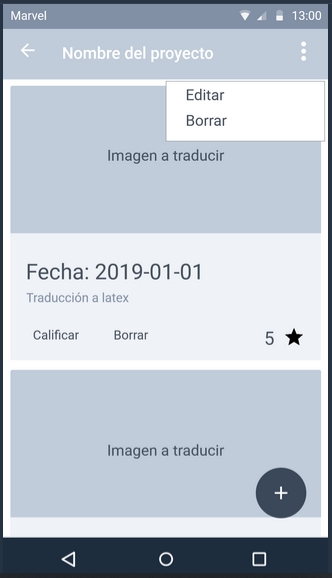
\includegraphics[width=200px]{capitulo4/imagenes/android/MIUA_6.png}
    \caption{MIUA 6 Lista de Traducciones}
    \label{fig:MIUA-6} %MOCK UP DE INTERFAZ DE USUARIO ANDROID
\end{figure}

\begin{figure}[H]
    \centering
    \includegraphics[width=200px]{capitulo4/imagenes/android/MIUA_7.png}
    \caption{MIUA 7 Editar Perfil}
    \label{fig:MIUA-7} %MOCK UP DE INTERFAZ DE USUARIO ANDROID
\end{figure}

\newpage
\subsection{Aplicación en Web}
\begin{figure}[H]
    \centering
    \includegraphics[width=300px]{capitulo4/imagenes/web/IUW_1.png}
    \caption{MIUW 1 Iniciar Sesión}
    \label{fig:MIUW-1}
\end{figure}

\begin{figure}[H]
    \centering
    \includegraphics[width=300px]{capitulo4/imagenes/web/IUW_2.png}
    \caption{MIUW 2 Registro}
    \label{fig:MIUW-2}
\end{figure}

\begin{figure}[H]
    \centering
    \includegraphics[width=300px]{capitulo4/imagenes/web/IUW_3.png}
    \caption{MIUW 3 Editar Perfil}
    \label{fig:MIUW-3}
\end{figure}

\begin{figure}[H]
    \centering
    \includegraphics[width=300px]{capitulo4/imagenes/web/IUW_4.png}
    \caption{MIUW 4 Recuperar Contraseña}
    \label{fig:MIUW-4}
\end{figure}

\begin{figure}[H]
    \centering
    \includegraphics[width=300px]{capitulo4/imagenes/web/IUW_5.png}
    \caption{MIUW 5 Lista de Proyectos}
    \label{fig:MIUW-5}
\end{figure}

\begin{figure}[H]
    \centering
    \includegraphics[width=300px]{capitulo4/imagenes/web/IUW_6.png}
    \caption{MIUW 6 Lista de Traducciones}
    \label{fig:MIUW-6}
\end{figure}

\begin{figure}[H]
    \centering
    \includegraphics[width=300px]{capitulo4/imagenes/web/IUW_7.png}
    \caption{MIUW 7 Menú de Opciones}
    \label{fig:MIUW-7}
\end{figure}

\chapter{Desarrollo del sistema}
%Esta parte me causa un poco de ruido, al parecer va todo el codigo y describir en que consiste todo lo que se realizo y para que sirve cada cosa

A continuación, se explica el desarrollo del sistema, dicha explicación se encuentra dividida en la sección del desarrollo de la aplicación móvil y por otra parte se encuentra el desarrollo de la aplicación web.

\section{Android}
Esta sección tiene objetivo presentar las principales características en el desarrollo de la aplicación para Android.
\subsection{Arquitectura de la aplicación}
Para el desarrollo de la aplicación se implemento la arquitectura Clean, la cual como ya se ha mencionado antes se ha mencionado se ha vuelto muy popular en el desarrollo de aplicaciones móviles para android debido a que es una solución que produce sistemas que presentan las siguientes características.

\begin{itemize}
    \item Escalables, por lo que se pueden agregar más funcionalidades de forma sencilla.
    \item Presentan modularidad.
    \item Presentan independencia en cuanto a frameworks, interfaz de usuario y bases de datos.
    \item El proyecto es más fácil de mantener por lo que es más sencillo hacer cambios.
\end{itemize}

Al utilizar esta arquitectura el proyecto queda separado en tres capas como se observa en la figura \ref{fig:capas-arquitectura} con lo cual cada una de ellas tiene su propósito definido.

\begin{figure}[h]
    \centering
    \includegraphics[width=250px]{capitulo5/android/img/capas-clean.png}
    \caption{Tres capas que se tienen al utilizar la arquitectura Clean \cite{cleanGuide}}
    \label{fig:capas-arquitectura}
\end{figure}

\subsubsection{Capa de datos}
La información que se utiliza en el resto de capas proviene de esta capa. Esta capa a su vez se encuentra dividida en la capa de repositorio y en la capa de fuente de datos. 

\paragraph{Capa de repositorio} En esta capa se utiliza el patrón de repositorio como se muestra en la figura \ref{fig:capa-datos}. Gracias a este patrón se puede tener acceso a diferentes fuentes de datos que se encuentran en la capa más baja de nuestra arquitectura, esto nos permite un acceso a los datos de forma transparente para el usuario bajo las condiciones que se presenten.

La forma de utilizar este patrón en la aplicación desarrollado crear una clase en la cual se hace uso de la interfaz que se tiene para el acceso a la fuente de datos. En el siguiente código se puede apreciar el como se crea una instancia de APIService que es nuestra interfaz para fuente de datos.

Después, en nuestro método findAllProyecttosByUser se recupera la información necesaria para mandarla a las capas superiores.

\lstinputlisting[language=Java]{capitulo5/android/src/repositorio.java}

\begin{figure}[h]
    \centering
    \includegraphics[width=400px]{capitulo5/android/img/capa-datos.png}
    \caption{Capa de datos \cite{cleanWay}}
    \label{fig:capa-datos}
\end{figure}

\paragraph{Capa de fuente de datos} En este trabajo, la fuente de datos que se tiene es un API REST, sin embargo si se requiere acceder a información que se persista en el teléfono se pude agregar otra fuente de datos. Se utilizó retrofit para poder realizar la comunicación con el API REST. 

La forma de utilizar retrofit es crear una interfaz con todos los métodos para recuperar o enviar información al API REST, en esta interfaz cada método tiene la URL a la cual se realizara la petición con alguno de los métodos que tiene HTTP, se tienen los parámetro que se envían y cada método nos regresa una llamada asíncrona que se trabaja en la capa de repositorio. Esto se puede apreciar en el siguiente código.

\lstinputlisting[language=Java]{capitulo5/android/src/APIService.java}

Para poder hacer uso de esta interfaz se tiene que configurar bajo ciertas características especificas como lo son la URL a la cual hará peticiones, el logger que se utilizara para poder observar las peticiones que se realizan y brindar una retroalimentación a la hora de hacer pruebas y por ultimo el parser que se utilizara para trabajar y pasar de clases a datos que el API REST entienda y pueda utilizar, en este caso se utilizo el formato JSON. La definición de estas características se tiene en el siguiente código.

\lstinputlisting[language=Java]{capitulo5/android/src/ServiceGenerator.java}

Finalmente, en esta capa se tienen clases Java que después se mapean a objetos JSON y viceversa, para realizar esto se crea un POJO con los atributos que se necesitan además de agregar anotaciones de retrofit para que el parser pude hacer la conversión necesaria. Un ejemplo de esto es en la siguiente clase de java.

\lstinputlisting[language=Java]{capitulo5/android/src/UsuarioData.java}


\subsubsection{Capa de dominio}
En esta capa es la intermediaria entre las otras dos capas que se tienen, es donde se encuentran los casos de uso también conocidos como interactors como se muestra en la figura \ref{fig:capa-dominio} en ellos la lógica del negocio es ejecutada es por esto que es el núcleo de la aplicación.

Es importante mencionar que esta capa, al ser la encargada del negocio es donde se hacen validaciones en la información y dicha información se adapta para que sea trabajada en la capa de presentación o en la de datos

Además de contener los casos de uso en esta capa se encuentran las entidades y se hace uso de los repositorios para acceder a la información proporcionada por la capa de datos.

\begin{figure}[h]
    \centering
    \includegraphics[width=200px]{capitulo5/android/img/capa-dominio.png}
    \caption{Capa de dominio \cite{cleanWay}}
    \label{fig:capa-dominio}
\end{figure}

Para tener un control sobre posibles errores en la capa de presentación o en la capa de datos se utilizan códigos de resultados al igual que una clase que contiene el resultado que se puede presentar, así como la información que se le regresa a la capa de presentación. Se hace uso de genéricos para poder reutilizar esta clase en toda la aplicación y no duplicar código. La clase es la siguiente.

\lstinputlisting[language=Java]{capitulo5/android/src/BusinessResult.java}

La forma en la que se utiliza esta clase en un caso de uso se presenta en el siguiente código que permite iniciar sesión.

\lstinputlisting[language=Java]{capitulo5/android/src/UserInteractorImpl.java}

A su vez el caso de uso utiliza sus propios clases de java para presentar información al usuario en la capa de presentación así como controlar posibles errores en la información que ingrese el usuario los campos de los formularios, un ejemplo de este tipo de clases es el siguiente.

\lstinputlisting[language=Java]{capitulo5/android/src/UsuarioModel.java}

\subsubsection{Capa de presentación}
En esta capa como se muestra en la figura \ref{fig:capa-presentacion} se trabaja con la lógica relacionada a las interfaces que se tienen en la aplicación, es decir a actividades, fragmentos y archivos XML.

\begin{figure}[h]
    \centering
    \includegraphics[width=300px]{capitulo5/android/img/capa-presentacion.png}
    \caption{Capa de presentación \cite{cleanWayReload}}
    \label{fig:capa-presentacion}
\end{figure}

En esta capa se pueden trabajar con patrones como MVC y MVP pero en este caso se utiliza el patrón MVVM cada uno con una función en particular. \cite{cleanWayReload}

\begin{itemize}
    \item \textbf{Modelo} Se encarga de representar la información que sera presentada en la vista.
    \item \textbf{Vista} Compuesta en este caso por las actividades y fragmentos de la aplicación, su tarea es mostrar la información, hacen uso de los viewmodels para poder realizar cambios en la interfaz.
    \item \textbf{ViewModel} El ViewModel sera el encargado de ejecutar los casos de uso o interactors con el objetivo de actualizar la vista de acuerdo a la información que presente el modelo.
\end{itemize}



\section{Android}
Esta sección tiene objetivo presentar las principales características en el desarrollo de la aplicación para Android.
\subsection{Arquitectura de la aplicación}
Para el desarrollo de la aplicación se implemento la arquitectura Clean, la cual como ya se ha mencionado antes se ha mencionado se ha vuelto muy popular en el desarrollo de aplicaciones móviles para android debido a que es una solución que produce sistemas que presentan las siguientes características.

\begin{itemize}
    \item Escalables, por lo que se pueden agregar más funcionalidades de forma sencilla.
    \item Presentan modularidad.
    \item Presentan independencia en cuanto a frameworks, interfaz de usuario y bases de datos.
    \item El proyecto es más fácil de mantener por lo que es más sencillo hacer cambios.
\end{itemize}

Al utilizar esta arquitectura el proyecto queda separado en tres capas como se observa en la figura \ref{fig:capas-arquitectura} con lo cual cada una de ellas tiene su propósito definido.

\begin{figure}[h]
    \centering
    \includegraphics[width=250px]{capitulo5/android/img/capas-clean.png}
    \caption{Tres capas que se tienen al utilizar la arquitectura Clean \cite{cleanGuide}}
    \label{fig:capas-arquitectura}
\end{figure}

\subsubsection{Capa de datos}
La información que se utiliza en el resto de capas proviene de esta capa. Esta capa a su vez se encuentra dividida en la capa de repositorio y en la capa de fuente de datos. 

\paragraph{Capa de repositorio} En esta capa se utiliza el patrón de repositorio como se muestra en la figura \ref{fig:capa-datos}. Gracias a este patrón se puede tener acceso a diferentes fuentes de datos que se encuentran en la capa más baja de nuestra arquitectura, esto nos permite un acceso a los datos de forma transparente para el usuario bajo las condiciones que se presenten.

La forma de utilizar este patrón en la aplicación desarrollado crear una clase en la cual se hace uso de la interfaz que se tiene para el acceso a la fuente de datos. En el siguiente código se puede apreciar el como se crea una instancia de APIService que es nuestra interfaz para fuente de datos.

Después, en nuestro método findAllProyecttosByUser se recupera la información necesaria para mandarla a las capas superiores.

\lstinputlisting[language=Java]{capitulo5/android/src/repositorio.java}

\begin{figure}[h]
    \centering
    \includegraphics[width=400px]{capitulo5/android/img/capa-datos.png}
    \caption{Capa de datos \cite{cleanWay}}
    \label{fig:capa-datos}
\end{figure}

\paragraph{Capa de fuente de datos} En este trabajo, la fuente de datos que se tiene es un API REST, sin embargo si se requiere acceder a información que se persista en el teléfono se pude agregar otra fuente de datos. Se utilizó retrofit para poder realizar la comunicación con el API REST. 

La forma de utilizar retrofit es crear una interfaz con todos los métodos para recuperar o enviar información al API REST, en esta interfaz cada método tiene la URL a la cual se realizara la petición con alguno de los métodos que tiene HTTP, se tienen los parámetro que se envían y cada método nos regresa una llamada asíncrona que se trabaja en la capa de repositorio. Esto se puede apreciar en el siguiente código.

\lstinputlisting[language=Java]{capitulo5/android/src/APIService.java}

Para poder hacer uso de esta interfaz se tiene que configurar bajo ciertas características especificas como lo son la URL a la cual hará peticiones, el logger que se utilizara para poder observar las peticiones que se realizan y brindar una retroalimentación a la hora de hacer pruebas y por ultimo el parser que se utilizara para trabajar y pasar de clases a datos que el API REST entienda y pueda utilizar, en este caso se utilizo el formato JSON. La definición de estas características se tiene en el siguiente código.

\lstinputlisting[language=Java]{capitulo5/android/src/ServiceGenerator.java}

Finalmente, en esta capa se tienen clases Java que después se mapean a objetos JSON y viceversa, para realizar esto se crea un POJO con los atributos que se necesitan además de agregar anotaciones de retrofit para que el parser pude hacer la conversión necesaria. Un ejemplo de esto es en la siguiente clase de java.

\lstinputlisting[language=Java]{capitulo5/android/src/UsuarioData.java}


\subsubsection{Capa de dominio}
En esta capa es la intermediaria entre las otras dos capas que se tienen, es donde se encuentran los casos de uso también conocidos como interactors como se muestra en la figura \ref{fig:capa-dominio} en ellos la lógica del negocio es ejecutada es por esto que es el núcleo de la aplicación.

Es importante mencionar que esta capa, al ser la encargada del negocio es donde se hacen validaciones en la información y dicha información se adapta para que sea trabajada en la capa de presentación o en la de datos

Además de contener los casos de uso en esta capa se encuentran las entidades y se hace uso de los repositorios para acceder a la información proporcionada por la capa de datos.

\begin{figure}[h]
    \centering
    \includegraphics[width=200px]{capitulo5/android/img/capa-dominio.png}
    \caption{Capa de dominio \cite{cleanWay}}
    \label{fig:capa-dominio}
\end{figure}

Para tener un control sobre posibles errores en la capa de presentación o en la capa de datos se utilizan códigos de resultados al igual que una clase que contiene el resultado que se puede presentar, así como la información que se le regresa a la capa de presentación. Se hace uso de genéricos para poder reutilizar esta clase en toda la aplicación y no duplicar código. La clase es la siguiente.

\lstinputlisting[language=Java]{capitulo5/android/src/BusinessResult.java}

La forma en la que se utiliza esta clase en un caso de uso se presenta en el siguiente código que permite iniciar sesión.

\lstinputlisting[language=Java]{capitulo5/android/src/UserInteractorImpl.java}

A su vez el caso de uso utiliza sus propios clases de java para presentar información al usuario en la capa de presentación así como controlar posibles errores en la información que ingrese el usuario los campos de los formularios, un ejemplo de este tipo de clases es el siguiente.

\lstinputlisting[language=Java]{capitulo5/android/src/UsuarioModel.java}

\subsubsection{Capa de presentación}
En esta capa como se muestra en la figura \ref{fig:capa-presentacion} se trabaja con la lógica relacionada a las interfaces que se tienen en la aplicación, es decir a actividades, fragmentos y archivos XML.

\begin{figure}[h]
    \centering
    \includegraphics[width=300px]{capitulo5/android/img/capa-presentacion.png}
    \caption{Capa de presentación \cite{cleanWayReload}}
    \label{fig:capa-presentacion}
\end{figure}

En esta capa se pueden trabajar con patrones como MVC y MVP pero en este caso se utiliza el patrón MVVM cada uno con una función en particular. \cite{cleanWayReload}

\begin{itemize}
    \item \textbf{Modelo} Se encarga de representar la información que sera presentada en la vista.
    \item \textbf{Vista} Compuesta en este caso por las actividades y fragmentos de la aplicación, su tarea es mostrar la información, hacen uso de los viewmodels para poder realizar cambios en la interfaz.
    \item \textbf{ViewModel} El ViewModel sera el encargado de ejecutar los casos de uso o interactors con el objetivo de actualizar la vista de acuerdo a la información que presente el modelo.
\end{itemize}



%\section{Conjunto de entrenamiento}
\subsection{Descripción}
Uno de los principales retos al trabajar con redes neuronales es la obtención de grandes conjuntos de entrenamiento que permitan mejores resultados, para el problema de reconocimiento de expresiones matemáticas existe una competencia llamada \textbf{Competition on Recognition of Online Handwritten Mathematical Expressions (CROHME)} que pone disponible de manera libre un conjunto de entrenamiento con mas de diez mil expresiones matemáticas escritas a mano provenientes de muchos usuarios voluntarios de distintos países mezclando los conjuntos de entrenamiento de 3 competencias CROHME. Se le pidió a los voluntarios copiar expresiones impresas de un \texttt{corpus} de expresiones. El corpus ha sido diseñado para cubrir la diversidad compuesta por las distintas tareas elegidas de un corpora matemático y de expresiones embebidas en páginas de wikipedia. Distintos dispositivos han sido utilizados (plumas digitales de distintas tecnologías, dispositivos de entrada como pizarrones blancos, tablets con pantalla sensible) de tal modo que distintas escalas y resoluciones son usadas %\cite{}.

\begin{figure}[h]
	\centering
	\includegraphics[width=0.4\textwidth]{capitulo5/dataset/crohme.jpg}
	\caption{Imagen de ejemplo del conjunto de datos de CROHME}
	\label{fig:crohme}
\end{figure}

A pesar de parecer un conjunto de datos prometedor para el desarrollo del presente trabajo terminal se deben considerar factores como el ruido que puede tener una imagen a partir de una fotografía tomada con un smartphone, por lo que se ha optado por utilizar una técnica denominada data aumentation que consiste en agregar ruido al conjunto de entrenamiento y otros procesos de análisis de imágenes como los mencionados en \ref{imAnalysis} permitiendo que el conjunto sea menos ideal y se puedan lograr mejores resultados 



\newpage
\section{Conjuntos de entrenamiento}

\subsection{CROHME}

El conjunto de datos de entrenamiento para el desarrollo de la red es el denominado \textbf{CROHME} por sus siglas en inglés: \textbf{Competition on Recognition of Online Handwritten Mathematical Expressions} publicado por los organizadores de la competencia internacional CROHME; para el caso del conjunto de entrenamiento fue posible reunir 7169 elementos que de acuerdo a investigación previa \cite{chino}, son relativamente pocos  para esperar una buena precisión, los  elementos en en el conjunto son archivos de tipo INKML.
\subsubsection{Formato del conjunto de datos}

Como ya se mencionó, los elementos del conjunto son archivos de tipo INKML (Ink Markup Language) y que principalmente se compone de tres partes:

\begin{itemize}
	\item Ink: Un conjunto de trazos definidos por puntos.
	\item Nivel de símbolo Ground-Truth: La segmentación e información de etiqueta de cada símbolo de la expresión.
	\item Ground-truth: La estructura MATHML de la expresión.
\end{itemize}

La información de \textit{Ground-Truth} tanto de nivel de símbolo como de la expresión matemática fueron ingresadas manualmente por los colaboradores de la generación del conjunto, además, alguna información general es agregada en el archivo:

\begin{itemize}
	\item Los canales (en este caso X, Y)
	\item La información del escritor (Identificación, entrega, edad, Mano dominante, género, etc ), si está disponible.
	\item Ground-Truth en \LaTeX{} para fácilmente renderizarlo.
\end{itemize} 

Es importante señalar que al pasar los archivos de INKML a imagen PNG, se obtuvieron imágenes de diferentes tamaños, sin embargo en el entrenamiento las imágenes que se utilizaron fueron de 300x150 px.

A continuación se muestra un ejemplo de un archivo del dataset que representa la expresión \$2 \^\ \{-1 \} \$:\\
 $2^{-1}$ renderizado.
\lstinputlisting[language=XML]{capitulo5/dataset/Inkdata_temp_InkFR_HPR_EQU_NOC_scc696_fi6_db144195.inkml}
Sin embargo, para el propósito del trabajo terminal, el conjunto de datos no es útil en este formato, por lo que se tenía que transformar la información de los trazos en imágenes.
\subsubsection{Conversión a imagen}
Con la información que contiene el archivo INKML es posible generar una imagen con los puntos de los trazos en negro y fondo blanco. El primer reto fue identificar las etiquetas que contenían a los trazos, para ello se utilizó la biblioteca de Python xml.etree y una función de terceros para poder utilizar dichos trazos posteriormente:

\lstinputlisting[language=Python]{capitulo5/dataset/getTraces.py}

Una vez obtenidos los trazos y con ayuda de matplotlib fueron separados como puntos $x,y$ y utilizados en la función plot de matplotlib para posteriormente guardarlo como imagen.

\lstinputlisting[language=Python]{capitulo5/dataset/inkml2img_short.py}

Este procedimiento tenía que realizarse por cada uno de los elementos del conjunto de entrenamiento, además de también extraer la expresión matemática encerrada entre las etiquetas \textbf{$<$annotation$>$$<$/annotation$>$} con el atributo \textbf{type}, para ello nuevamente se utilizó la biblioteca de python xml.etree para acceder a los nodos del árbol directamente:
\lstinputlisting[language=Python]{capitulo5/dataset/tag.py}
Con estos subscripts fue posible desarrollar una biblioteca que permite acceder a la carpeta con el conjunto de entrenamiento en formato inkml y guardarlos como imagen en otra carpeta junto con un archivo CSV conteniendo la ruta relativa de la imagen y la expresión en \LaTeX{} correspondiente separados por coma.

\lstinputlisting[language=Python, firstline = 1, lastline=10]{capitulo5/dataset/training.csv}
\subsubsection{Generador de secuencia de tokens}
El archivo CSV generado con lo descrito anteriormente no es suficiente para cargarlo en TensorFlow, la expresión matemática en \LaTeX{} debía ser expresada como una secuencia numérica, por lo que se necesitaba identificar a cada símbolo con un número único y conformar a la secuencia, de modo que la estructura del archivo CSV pasaría de tener la forma \textbf{RUTA\_IMAGEN}, \textbf{EXPRESION\_LATEX} a tener la forma \textbf{RUTA\_IMAGEN}, \textbf{SECUENCIA\_NUMÉRICA}, teniendo así una nueva representación del conjunto de entrenamiento conformada por una carpeta con las imágenes y un archivo CSV previamente descrito para poder cargarse en TensorFlow.

Para esto, se desarrolló gracias a lex en Python un script para especificar los tokens tomando como base los símbolos especificados en la sección \ref{sec:del_exp}.\\\\
\lstinputlisting[language=Python, lastline=10]{capitulo5/dataset/Rules.py}

\lstinputlisting[language=Python, firstline = 26, lastline=44]{capitulo5/dataset/Analyzer.py}

\lstinputlisting[firstline = 1, lastline=10]{capitulo5/dataset/tokenized_training.csv}

\vspace{1em}
Es importante destacar que se debe también guardar este mapeo único y no alterar el orden, por lo que de requerir agregar nuevos símbolos al conjunto es necesario hacerlo al final de los ya existentes, ya que la red entrenada devuelve secuencias numéricas que deben mapearse para tener la correspondiente expresión en \LaTeX{}.

\subsection{Harvard 100k}

El segundo conjunto de entrenamiento utilizado fue el provisto por \cite{harvard}. Los investigadores que realizaron el paper liberaron el conjunto de entrenamiento que recabaron, el cual cuenta con alrededor de cien mil expresiones matemáticas escritas a computadora.

Este conjunto de entrenamiento puede descargarse libremente en la página provista por el artículo. Consiste en un conjunto de imágenes png sin preprocesar y sus respectivos resultados esperados (Grounth-Truth). Así mismo, los autores del artículo proveen scripts de normalización y de preprocesado para el tratamiento de las imágenes. Estos scripts se pueden encontrar en el github del artículo \cite{harvard-scripts}.

Se procedio a preprocesar las imágenes con los scripts provistos por los investigadores de Harvard y se obtuvo un conjunto de entrenamiento con 78000 imágenes. Debido a que en el presente Trabajo Terminal las estructuras matriciales no estan contempladas, se descartaron todas las imágenes que contuvieran matrices, arreglos o listas, así como aquellas que produjeron errores tras ser procesadas. El conjunto final contiene 73000 imágenes de distintos tamaños los cuales son: (200,50), (240,40), (280,40), (360,60), (160,40), (360,50), (120,50), (320,50), (400,50), (360,10), (360,40), (200,40), (320,40), (280,50) y (240,50). En la Figura \ref{fig:harvard-example} se puede ver un ejemplo de una imagen del conjunto de entrenamiento de Harvard.

\begin{figure}[H]
	\centering
	\includegraphics{capitulo5/dataset/harvard}
	\caption{Ejemplo de una imagen del conjunto de entrenamiento Harvard 100k}
	\label{fig:harvard-example}
\end{figure}

\subsection{Normalización}

Entre los scripts provistos por los investigadores de Harvard \cite{harvard-scripts}, se encuentra un normalizador. Este código, realiza una serie de transformaciones seguras con el fin de estandarizar ciertas inconsitencias con las expresiones en \LaTeX{}. Un ejemplo podría ser las distintas formas que se tienen para expresar un exponente: \textit{a \^\ b} y \textit{a \^\ \{ b \}} producirían el mismo resultado. Para mejorar el rendimiento de la red, ambos conjuntos de entrenamiento fueron preprocesados con el script de normalizado.

Cabe mencionar que ambos conjuntos de entrenamiento fueron unificados mediante la combinación de su Grounth-Truth, por lo que es posible utilizarlos indistintamente. Para unificarlos se proceso el conjunto CROHME para convertir sus tokens en tokens del conjunto de Harvard. El código usado se muestra a continuación.

\lstinputlisting[language=Python]{capitulo5/dataset/converter.py}

\newpage



\section{Desarrollo módulo de análisis de imágenes}

Las imágenes generadas para el conjunto de entrenamiento se formaron insertando los puntos en fondo blanco, teniendo como resultado una imagen binaria (contenido en negro y fondo blanco) por lo que al considerar que las fotogragías tomadas por un dispositivo móvil no iba a generar por sí mismo un formato semejante fue necesario desarrollar un módulo para esta tarea.

\begin{figure}[h]
	\centering
	\includegraphics[width=0.4\textwidth]{capitulo5/imageprocessor/example_dataset.png}
	\caption{Imagen de ejemplo del conjunto de entrenamiento generado}
	\label{fig:example_dataset}
\end{figure}

El proceso consiste en convertir el área de la expresión matemática en negro y el resto en fondo blanco, para ello se consideraron las técnicas mencionadas en %ref
 y específicamente se probaron los algoritmos de Otsu y Sauvola \cite{inproceedings}.
 
\begin{figure}[h]
	\centering
	\includegraphics[width=0.8\textwidth]{capitulo5/imageprocessor/IO_image.jpg}
	\caption{Fotografía procesada con algoritmo de Sauvola}
	\label{fig:process_image}
\end{figure}

De acuerdo a lo mencionado en el marco teórico existen técnicas para binarizar una imagen que calculan el umbral de manera automática, dos de estos algoritmos son el algoritmo de Otsu y el algoritmo de Sauvola, a continuación se describen brevemente y se dan detalles de la implementación o uso según el caso.

\subsection{Algoritmo de Otsu}
El método de Otsu evita tener que elegir un valor de umbral y lo determina automáticamente.

Considere una imagen con solos dos valores distintos (imagen bimodal), donde el histograma consistiría solo de dos picos. Un buen valor de umbral sería a la mitad de estos dos valores. Similarmente el método de Otsu determina un valor de umbral óptimo global del histograma de la imagen.

Al tratarse de una imagen bimodal, el algoritmo intenta encontrar un valor de umbral (t) que minimice la varianza ponderada dentro de la clase, dada por la relación:

\begin{equation}
	\sigma _ {w} ^{2}(t) = q_{1}(t) \sigma _{1}^2(t) + q_{2}(t) \sigma _{2}^2(t)
\end{equation}
donde:
\begin{equation}
	\begin{array}{l}
		q_{1}(t) = \sum_{i=1}^{t} P(i) \wedge q_{2}(t) = \sum_{i=t+1}^{I} P(i)\\\\
		\mu_{1}(t) = \sum_{i=1}^{t} \frac{i P(i)}{q_1{t}} \wedge \mu_{2}(t) = \sum_{i=t+1}^{I} \frac{i P(i)}{q_2{t}}\\\\
		\sigma_{1}^2(t) = \sum_{i = 1}^{t} [i - \mu_{1}(t)]^2 \frac{P(i)}{q_{1}(t)} \wedge \sigma_{2}^2(t) = \sum_{i = t+1}^{I} [i - \mu_{2}(t)]^2 \frac{P(i)}{q_{2}(t)}
	\end{array}
\end{equation}

\lstinputlisting[language=Python]{capitulo5/imageprocessor/code_files/otsu.py}

\subsection{Algoritmo de Sauvola}

El algorimo de Sauvola tiene una implementación más extensa por lo que se dispuso de la utilización de la implementación contenida en \textbf{skimage} dentro del paquete filters.
\lstinputlisting[language=Python, firstline=4, lastline=7]{capitulo5/imageprocessor/code_files/scriptCV.py}

\lstinputlisting[language=Python, firstline=26, lastline=30]{capitulo5/imageprocessor/code_files/scriptCV.py}

\chapter{Pruebas}

Lo más seguro es que tengamos que inlcuir el siguiente conjunto de pruebas

\begin{enumerate}
    \item Unitarias
    \item De integración
    \item De los requerimientos no funcionales
    \item Y principalmente con la arquitectura de la red neuronal y el conjunto de entrenamiento y con inputs esperados por el usuario
\end{enumerate}{}
\chapter{Conclusiones}
La detección de expresiones matemáticas escritas a mano es un problema difícil debido a la estructura jerárquica y bidimensional que presentan y a la ambigüedad inherente de la escritura a mano haciendo de este un problema de investigación abierto. Conscientes de esto, vimos la oportunidad de realizar un prototipo que busque dar solución al problema y a su vez tenga una utilidad para los usuarios de \LaTeX.

Los requerimientos funcionales planteados para la aplicación web y android se lograron alcanzar a través de un correcto análisis y diseño lo cual permitió que su desarrollo fuera lo más ágil posible al elegir las mejores tecnologías para su elaboración de acuerdo a las necesidades que se tenían.

Por otro lado, utilizar el algoritmo Sauvola para la binarización por sobre Otsu fue buena elección ya que presentó mejores resultados en las diferentes pruebas que se realizaron, permitió hacer que la imágenes que se toman con la cámara del teléfono fueran semejantes a las que se presentan en el conjunto de entrenamiento.

Con respecto al módulo de traducción de expresiones matemáticas no se llegó a una precisión requerida para llevar lo desarrollado a un ambiente de producción, debido a que dicha precisión está directamente afectada por el conjunto de entrenamiento. En el caso de las expresiones escritas a mano un conjunto con una mayor cantidad de imágenes podría mejorar significativamente los resultados del trabajo realizado, esto de acuerdo a la precisión obtenida con imágenes renderizadas por computadora en cuyo caso el conjunto de entrenamiento es al menos 10 veces mayor a su contraparte de expresiones escritas a mano, no se detectó otra posible solución a este problema ya que incluso probando variaciones en la red neuronal los resultados no mejoraron para expresiones escritas a mano.

Finalmente y tomando en cuenta lo anterior, varios puntos plateados en un inicio del trabajo terminal se lograron cubrir, sin embargo, el reconocimiento y traducción de las expresiones matemáticas escritas a mano es un problema aún no resuelto y por ende se puede trabajar más en buscar nuevas alternativas que brinden mejores resultados a los obtenidos en el presente trabajo terminal.

\chapter{Trabajo futuro}

La tarea primordial consiste en incrementar el conjunto de entrenamiento de expresiones matemáticas escritas a mano para que la cantidad de ejemplos disponibles sea similar al de conjunto de entrenamiento Harvard 100k.

Una forma de alcanzar este nuevo objetivo es el proporcionar al usuario la oportunidad de brindar retroalimentación a través de correcciones que se hagan a traducciones hechas por el sistema.

Esto se puede implementar en la parte android y el la parte web para que la funcionalidad de estas dos aplicaciones aumente. Además de buscar el llevar a producción estas dos aplicaciones una vez que se tenga un mejor resultado.

El proporcionar la oportunidad para un ambiente colaborativo en la gestión de proyectos para muchos usuarios y no solo la gestión de proyectos individuales agregará mayor valor al trabajo.

Probar el modelo desarrollado en el concurso CROHME de donde se obtuvo el conjunto de entrenamiento, el objetivo de dicho concurso se centra en el reconocimiento de expresiones matemáticas reconocidas a mano.


%\chapter{Glosario de términos} 



%%%%%%%%%%%%%%%%%%%%%%%%%%%%%%%%%%%%%%%%%%%%%%%%%%%%%
%                   APÉNDICES                       %
%%%%%%%%%%%%%%%%%%%%%%%%%%%%%%%%%%%%%%%%%%%%%%%%%%%%%
\appendix
%\include{Apendice1/Apendice1}               % Colocar los circuitos, manuales, código fuente, pruebas de teoremas, etc.

%%%%%%%%%%%%%%%%%%%%%%%%%%%%%%%%%%%%%%%%%%%%%%%%%%%%%
%                   REFERENCIAS                     %
%%%%%%%%%%%%%%%%%%%%%%%%%%%%%%%%%%%%%%%%%%%%%%%%%%%%%
% existen varios estilos de bilbiografía, pueden cambiarlos a placer
\bibliographystyle{ieeetr} % otros estilos pueden ser abbrv, acm, alpha, apalike, ieeetr, plain, siam, unsrt

%El formato trae otros estilos, o pueden agregar uno que les guste:
%\bibliographystyle{Latex/Classes/PhDbiblio-case} % title forced lower case
%\bibliographystyle{Latex/Classes/PhDbiblio-bold} % title as in bibtex but bold
%\bibliographystyle{Latex/Classes/PhDbiblio-url} % bold + www link if provided
%\bibliographystyle{Latex/Classes/jmb} % calls style file jmb.bst

\bibliography{bibliografia/referencias}             % Archivo .bib

\end{document}
